\documentclass[a4paper,12pt,twoside]{memoir}

% Castellano
\usepackage[spanish,es-tabla]{babel}
\selectlanguage{spanish}
\usepackage[utf8]{inputenc}
\usepackage[T1]{fontenc}
\usepackage{lmodern} % Scalable font
\usepackage{microtype}
\usepackage{placeins}

\RequirePackage{booktabs}
\RequirePackage[table]{xcolor}
\RequirePackage{xtab}
\RequirePackage{multirow}

% Links
\PassOptionsToPackage{hyphens}{url}\usepackage[colorlinks]{hyperref}
\hypersetup{
	allcolors = {blue}
}

% Ecuaciones
\usepackage{amsmath}

% Rutas de fichero / paquete
\newcommand{\ruta}[1]{{\sffamily #1}}

% Párrafos
\nonzeroparskip

% Huérfanas y viudas
\widowpenalty100000
\clubpenalty100000

% Imágenes

% Comando para insertar una imagen en un lugar concreto.
% Los parámetros son:
% 1 --> Ruta absoluta/relativa de la figura
% 2 --> Texto a pie de figura
% 3 --> Tamaño en tanto por uno relativo al ancho de página
\usepackage{graphicx}
\newcommand{\imagen}[3]{
	\begin{figure}[!h]
		\centering
		\includegraphics[width=#3\textwidth]{#1}
		\caption{#2}\label{fig:#1}
	\end{figure}
	\FloatBarrier
}

% Comando para insertar una imagen sin posición.
% Los parámetros son:
% 1 --> Ruta absoluta/relativa de la figura
% 2 --> Texto a pie de figura
% 3 --> Tamaño en tanto por uno relativo al ancho de página
\newcommand{\imagenflotante}[3]{
	\begin{figure}
		\centering
		\includegraphics[width=#3\textwidth]{#1}
		\caption{#2}\label{fig:#1}
	\end{figure}
}

% El comando \figura nos permite insertar figuras comodamente, y utilizando
% siempre el mismo formato. Los parametros son:
% 1 --> Porcentaje del ancho de página que ocupará la figura (de 0 a 1)
% 2 --> Fichero de la imagen
% 3 --> Texto a pie de imagen
% 4 --> Etiqueta (label) para referencias
% 5 --> Opciones que queramos pasarle al \includegraphics
% 6 --> Opciones de posicionamiento a pasarle a \begin{figure}
\newcommand{\figuraConPosicion}[6]{%
  \setlength{\anchoFloat}{#1\textwidth}%
  \addtolength{\anchoFloat}{-4\fboxsep}%
  \setlength{\anchoFigura}{\anchoFloat}%
  \begin{figure}[#6]
    \begin{center}%
      \Ovalbox{%
        \begin{minipage}{\anchoFloat}%
          \begin{center}%
            \includegraphics[width=\anchoFigura,#5]{#2}%
            \caption{#3}%
            \label{#4}%
          \end{center}%
        \end{minipage}
      }%
    \end{center}%
  \end{figure}%
}

%
% Comando para incluir imágenes en formato apaisado (sin marco).
\newcommand{\figuraApaisadaSinMarco}[5]{%
  \begin{figure}%
    \begin{center}%
    \includegraphics[angle=90,height=#1\textheight,#5]{#2}%
    \caption{#3}%
    \label{#4}%
    \end{center}%
  \end{figure}%
}
% Para las tablas
\newcommand{\otoprule}{\midrule [\heavyrulewidth]}
%
% Nuevo comando para tablas pequeñas (menos de una página).
\newcommand{\tablaSmall}[5]{%
 \begin{table}
  \begin{center}
   \rowcolors {2}{gray!35}{}
   \begin{tabular}{#2}
    \toprule
    #4
    \otoprule
    #5
    \bottomrule
   \end{tabular}
   \caption{#1}
   \label{tabla:#3}
  \end{center}
 \end{table}
}

%
% Nuevo comando para tablas pequeñas (menos de una página).
\newcommand{\tablaSmallSinColores}[5]{%
 \begin{table}[H]
  \begin{center}
   \begin{tabular}{#2}
    \toprule
    #4
    \otoprule
    #5
    \bottomrule
   \end{tabular}
   \caption{#1}
   \label{tabla:#3}
  \end{center}
 \end{table}
}

\newcommand{\tablaApaisadaSmall}[5]{%
\begin{landscape}
  \begin{table}
   \begin{center}
    \rowcolors {2}{gray!35}{}
    \begin{tabular}{#2}
     \toprule
     #4
     \otoprule
     #5
     \bottomrule
    \end{tabular}
    \caption{#1}
    \label{tabla:#3}
   \end{center}
  \end{table}
\end{landscape}
}

%
% Nuevo comando para tablas grandes con cabecera y filas alternas coloreadas en gris.
\newcommand{\tabla}[6]{%
  \begin{center}
    \tablefirsthead{
      \toprule
      #5
      \otoprule
    }
    \tablehead{
      \multicolumn{#3}{l}{\small\sl continúa desde la página anterior}\\
      \toprule
      #5
      \otoprule
    }
    \tabletail{
      \hline
      \multicolumn{#3}{r}{\small\sl continúa en la página siguiente}\\
    }
    \tablelasttail{
      \hline
    }
    \bottomcaption{#1}
    \rowcolors {2}{gray!35}{}
    \begin{xtabular}{#2}
      #6
      \bottomrule
    \end{xtabular}
    \label{tabla:#4}
  \end{center}
}

%
% Nuevo comando para tablas grandes con cabecera.
\newcommand{\tablaSinColores}[6]{%
  \begin{center}
    \tablefirsthead{
      \toprule
      #5
      \otoprule
    }
    \tablehead{
      \multicolumn{#3}{l}{\small\sl continúa desde la página anterior}\\
      \toprule
      #5
      \otoprule
    }
    \tabletail{
      \hline
      \multicolumn{#3}{r}{\small\sl continúa en la página siguiente}\\
    }
    \tablelasttail{
      \hline
    }
    \bottomcaption{#1}
    \begin{xtabular}{#2}
      #6
      \bottomrule
    \end{xtabular}
    \label{tabla:#4}
  \end{center}
}

%
% Nuevo comando para tablas grandes sin cabecera.
\newcommand{\tablaSinCabecera}[5]{%
  \begin{center}
    \tablefirsthead{
      \toprule
    }
    \tablehead{
      \multicolumn{#3}{l}{\small\sl continúa desde la página anterior}\\
      \hline
    }
    \tabletail{
      \hline
      \multicolumn{#3}{r}{\small\sl continúa en la página siguiente}\\
    }
    \tablelasttail{
      \hline
    }
    \bottomcaption{#1}
  \begin{xtabular}{#2}
    #5
   \bottomrule
  \end{xtabular}
  \label{tabla:#4}
  \end{center}
}



\definecolor{cgoLight}{HTML}{EEEEEE}
\definecolor{cgoExtralight}{HTML}{FFFFFF}

%
% Nuevo comando para tablas grandes sin cabecera.
\newcommand{\tablaSinCabeceraConBandas}[5]{%
  \begin{center}
    \tablefirsthead{
      \toprule
    }
    \tablehead{
      \multicolumn{#3}{l}{\small\sl continúa desde la página anterior}\\
      \hline
    }
    \tabletail{
      \hline
      \multicolumn{#3}{r}{\small\sl continúa en la página siguiente}\\
    }
    \tablelasttail{
      \hline
    }
    \bottomcaption{#1}
    \rowcolors[]{1}{cgoExtralight}{cgoLight}

  \begin{xtabular}{#2}
    #5
   \bottomrule
  \end{xtabular}
  \label{tabla:#4}
  \end{center}
}



\graphicspath{ {./img/} }

% Capítulos
\chapterstyle{bianchi}
\newcommand{\capitulo}[2]{
	\setcounter{chapter}{#1}
	\setcounter{section}{0}
	\setcounter{figure}{0}
	\setcounter{table}{0}
	\chapter*{\thechapter.\enskip #2}
	\addcontentsline{toc}{chapter}{\thechapter.\enskip #2}
	\markboth{#2}{#2}
}

% Apéndices
\renewcommand{\appendixname}{Apéndice}
\renewcommand*\cftappendixname{\appendixname}

\newcommand{\apendice}[1]{
	%\renewcommand{\thechapter}{A}
	\chapter{#1}
}

\renewcommand*\cftappendixname{\appendixname\ }

% Formato de portada
\makeatletter
\usepackage{xcolor}
\newcommand{\tutor}[1]{\def\@tutor{#1}}
\newcommand{\tutors}[1]{\def\@tutors{#1}}
\newcommand{\course}[1]{\def\@course{#1}}
\definecolor{cpardoBox}{HTML}{E6E6FF}
\def\maketitle{
  \null
  \thispagestyle{empty}
  % Cabecera ----------------
\noindent
\includegraphics[width=\textwidth]{cabecera}\vspace{1cm}%
  \vfill
  % Título proyecto y escudo informática ----------------
  \colorbox{cpardoBox}{%
    \begin{minipage}{.8\textwidth}
      \vspace{.5cm}\Large
      \begin{center}
      \textbf{TFG del Grado en Ingeniería Informática}\vspace{.6cm}\\
      \textbf{\LARGE\@title{}}
      \end{center}
      \vspace{.2cm}
    \end{minipage}

  }%
  \hfill\begin{minipage}{.20\textwidth}
    
\includegraphics[width=\textwidth]{escudoInfor}
  \end{minipage}
  \vfill
  % Datos de alumno, curso y tutores ------------------
  \begin{center}%
  {%
    \noindent\LARGE
    Presentado por \@author{}\\ 
    en Universidad de Burgos --- \@date{}\\
    Tutor: \@tutor{}\\
	Tutor: \@tutors{}\\
  }%
  \end{center}%
  \null
  \cleardoublepage
  }
\makeatother

\newcommand{\nombre}{José Luis Caballero Martínez-Quintanilla} %%% cambio de comando

% Datos de portada
\title{Diseño de un sistema económico IoT de monitorización de invernaderos de cannabis medicinal}
\author{\nombre}
\tutor{Alejandro Merino Gómez}
\tutors{Carlos Cambra Baseca}
\date{16 de febrero de 2024}

\begin{document}

\maketitle


\newpage\null\thispagestyle{empty}\newpage


%%%%%%%%%%%%%%%%%%%%%%%%%%%%%%%%%%%%%%%%%%%%%%%%%%%%%%%%%%%%%%%%%%%%%%%%%%%%%%%%%%%%%%%%
\thispagestyle{empty}


\noindent
\includegraphics[width=\textwidth]{cabecera}\vspace{1cm}

\noindent D. Alejandro Merino Gómez, profesor del departamento de Digitalización, área de Systems Engineering and Automation y D. Carlos Cambra Baseca, profesor del departamento de Digitalización del área de Computer Science and Artificial Intelligence, 

\noindent Exponen:

\noindent Que el alumno D. \nombre, con DNI 48471169-A, ha realizado el Trabajo final de Grado en Ingeniería Informática titulado Diseño de un sistema económico IoT de monitorización de invernaderos de cannabis medicinal. 

\noindent Y que dicho trabajo ha sido realizado por el alumno bajo la dirección del que suscribe, en virtud de lo cual se autoriza su presentación y defensa.

\begin{center} %\large
En Burgos, {\large 16 de febrero de 2024}
\end{center}

\vfill\vfill\vfill

% Author and supervisor
\begin{minipage}{0.45\textwidth}
\begin{flushleft} %\large
Vº. Bº. del Tutor:\\[2cm]
D. Merino Gómez, Alejandro
\end{flushleft}
\end{minipage}
\hfill
\begin{minipage}{0.45\textwidth}
\begin{flushleft} %\large
Vº. Bº. del co-tutor:\\[2cm]
D. Cambra Baseca, Carlos 
\end{flushleft}
\end{minipage}
\hfill

\vfill

% para casos con solo un tutor comentar lo anterior
% y descomentar lo siguiente
%Vº. Bº. del Tutor:\\[2cm]
%D. nombre tutor


\newpage\null\thispagestyle{empty}\newpage




\frontmatter

% Abstract en castellano
\renewcommand*\abstractname{Resumen}
\begin{abstract}
El presente trabajo de fin de grado aborda el diseño de un sistema económico basado en el Internet de las cosas (IoT) para la monitorización de invernaderos destinados al cultivo de cannabis medicinal. El objetivo principal es mejorar la eficiencia y la calidad del cultivo mediante la implementación de sensores y dispositivos conectados que permitan la recolección y análisis de datos en tiempo real.

El hardware seleccionado para este proyecto incluye la Raspberry Pi Pico W como unidad central, una pantalla OLED 128x64 para la visualización de información, el sensor DHT22 para la medición de la temperatura y humedad ambiente, el sensor BH1750 para evaluar la intensidad lumínica, y un sensor de humedad de suelo para monitorear las condiciones de la tierra.

A lo largo del trabajo, se detalla el proceso de integración de estos componentes, se describen las tecnologías utilizadas para la comunicación y el manejo de datos, y se presenta la interfaz de usuario diseñada para la visualización de información relevante. Se destacan también las consideraciones económicas que han llevado a la elección de cada componente, buscando una solución asequible sin comprometer la calidad de los resultados.

Los resultados obtenidos demuestran la viabilidad y eficacia del sistema propuesto, ofreciendo a los agricultores de cannabis medicinal un instrumento práctico y accesible para mejorar la gestión de sus invernaderos. Este trabajo contribuye al campo emergente de la agricultura inteligente y sostenible, abriendo posibilidades para futuras investigaciones y aplicaciones en el ámbito de la monitorización agrícola basada en IoT.

\end{abstract}

\renewcommand*\abstractname{Descriptores}
\begin{abstract}
Raspberry Pi Pico W, Micropython, Autónomo, Sistema Domótico, Bot, Telegram, Python \ldots
\end{abstract}

\clearpage

% Abstract en inglés
\renewcommand*\abstractname{Abstract}
\begin{abstract}
This project deals with the design of an economic system based on the Internet of Things (IoT) for the monitoring of greenhouses for the cultivation of medical cannabis. The main objective is to improve the efficiency and quality of the crop through the implementation of sensors and connected devices that allow the collection and analysis of data in real time.

The hardware selected for this project includes the Raspberry Pi Pico W as the central unit, a 128x64 OLED screen for displaying information, the DHT22 sensor for measuring ambient temperature and humidity, the BH1750 sensor for evaluating light intensity, and a soil moisture sensor for monitoring soil conditions.

Throughout the paper, the integration process of these components is detailed, the technologies used for communication and data management are described, and the user interface designed for the visualization of relevant information is presented. It also highlights the economic considerations that led to the choice of each component, seeking an affordable solution without compromising the quality of the results.

The results obtained demonstrate the feasibility and effectiveness of the proposed system, offering medical cannabis farmers a practical and accessible tool to improve the management of their greenhouses. This work contributes to the emerging field of smart and sustainable agriculture, opening possibilities for future research and applications in the field of IoT-based agricultural monitoring.
\end{abstract}

\renewcommand*\abstractname{Keywords}
\begin{abstract}
Raspberry Pi Pico W, Micropython, Autonomous, Domotic System, Bot, Telegram, Python \ldots
\end{abstract}

\clearpage

% Indices
\tableofcontents

\clearpage

\listoffigures

\clearpage

\listoftables
\clearpage

\mainmatter
\capitulo{1}{Introducción}

El panorama en constante cambio de la industria del cannabis medicinal ha generado una creciente necesidad de optimizar los métodos de cultivo para garantizar la consistencia y calidad de los productos. En este contexto, el Internet de las cosas (IoT) emerge como una herramienta clave para transformar la gestión de invernaderos, permitiendo una monitorización en tiempo real y decisiones informadas por parte de los agricultores.

Este trabajo se centra en el diseño de un sistema asequible de monitorización basado en IoT para invernaderos de cannabis medicinal. La elección de hardware, liderada por la Raspberry Pi Pico W como unidad central, se fundamenta en la capacidad de esta plataforma para equilibrar eficiencia y costos. Sensores especializados, como el DHT22 para temperatura y humedad, el BH1750 para intensidad lumínica, y un sensor de humedad de suelo, complementan la infraestructura del hardware.

A través de un servidor LAMP, se centraliza la recopilación de datos en una base de datos para consultas históricas, mientras que MQTT facilita la obtención de datos en tiempo real. La información recabada puede ser visualizada de diversas maneras. Una pantalla OLED incorporada in situ en el invernadero ofrece una visualización local de los datos. Asimismo, un bot de Telegram permite interactuar mediante comandos o recibir alertas programadas, posibilitando una gestión remota eficiente.

Además, se dispone de un dashboard web que posibilita la visualización de datos tanto en tiempo real como en su historial. Complementando estas opciones, una aplicación de escritorio para Windows ofrece flexibilidad al permitir la visualización de datos en tiempo real y acceso al historial, además de proporcionar la capacidad de enviar comandos a la Raspberry Pi Pico W para activar mecanismos vinculados a las variables medidas. Esta diversidad de interfaces asegura que los usuarios tengan opciones versátiles para interactuar con el sistema de monitorización, adaptándose a sus necesidades específicas y facilitando la gestión efectiva del invernadero.

También se identificó la necesidad de utilizar Python para llevar a cabo la limpieza de datos y generar un resumen estadístico básico. A medida que la cantidad de datos aumente, se vislumbra la oportunidad de explorar posibilidades más avanzadas y significativas en el análisis de la información recopilada. Este enfoque proporciona una base sólida para futuras investigaciones y mejoras, permitiendo una evolución progresiva en la interpretación y aprovechamiento de los datos generados por el sistema.

Más allá de la mejora en la eficiencia del cultivo de cannabis medicinal, este proyecto busca situarse en la vanguardia de la agricultura inteligente y sostenible. La combinación de IoT con prácticas agrícolas avanzadas tiene el potencial de transformar radicalmente la forma en que se gestionan los cultivos, promoviendo la sostenibilidad y ofreciendo una solución práctica para agricultores de diversos niveles de recursos.

En resumen, este trabajo se adentra en el diseño de un sistema completo y accesible para la monitorización de invernaderos, utilizando la innovación tecnológica como catalizador para mejorar la calidad de los cultivos y contribuir al avance de la agricultura moderna.

\capitulo{2}{Objetivos del proyecto}
%Este apartado explica de forma precisa y concisa cuales son los objetivos que se persiguen con la realización del proyecto. Se puede distinguir entre los objetivos marcados por los requisitos del software a construir y los objetivos de carácter técnico que plantea a la hora de llevar a la práctica el proyecto.
\section{Objetivos del Software}
\begin{itemize}
\item \textbf{Desarrollo del Sistema de Adquisición de Datos:}
Implementar un sistema eficiente de adquisición de datos que pueda recopilar información precisa proveniente de los sensores (DHT22, BH1750, sensor de humedad de suelo) instalados en el invernadero.
\item \textbf{Diseño de la Interfaz de Usuario:}
Desarrollar una interfaz de usuario intuitiva y fácil de usar, que permita a los usuarios visualizar en tiempo real los datos recopilados y tomar decisiones informadas sobre el control del entorno del invernadero.
\item \textbf{Implementación de Protocolos de Comunicación:}
Establecer protocolos de comunicación eficientes para la transmisión de datos entre los sensores y la Raspberry Pi Pico W, así como para la conexión con otros dispositivos o sistemas externos si es necesario.
\end{itemize}
\pagebreak

\section{Objetivos Técnicos}
\begin{itemize}
\item \textbf{Integración de Hardware:} 
Seleccionar, configurar e integrar de manera óptima el hardware necesario (Raspberry Pi Pico W, pantalla OLED 128x64, sensores) para garantizar la estabilidad y la eficacia del sistema.

\item \textbf{Eficiencia Energética:}
Implementar estrategias de programación y configuración de hardware que optimicen el consumo de energía, asegurando una operación sostenible del sistema en entornos con recursos limitados. Precisamente la Raspberry Pi Pico W es conocida por su bajo consumo energético.

\item \textbf{Validación en Entorno Real:}
Realizar pruebas exhaustivas del sistema en un entorno de cultivo de cannabis medicinal real, evaluando su rendimiento, confiabilidad y adaptabilidad a condiciones variables.

\item \textbf{Consideraciones Económicas:}
Evaluar y optimizar los costos asociados al desarrollo e implementación del sistema, garantizando la viabilidad económica para agricultores de diferentes escalas y recursos.

\item \textbf{Documentación Completa:}
Generar una documentación detallada que abarque el diseño, la implementación y la configuración del sistema, facilitando la comprensión y la replicación por parte de otros interesados.
Estos objetivos, tanto del software como técnicos, se plantean con el propósito de cumplir con los requisitos del proyecto y garantizar la efectividad y utilidad del sistema de monitorización propuesto para invernaderos de cannabis medicinal.
\end{itemize}

\capitulo{3}{Conceptos teóricos}

%En aquellos proyectos que necesiten para su comprensión y desarrollo de unos conceptos teóricos de una determinada materia o de un determinado dominio de conocimiento, debe existir un apartado que sintetice dichos conceptos.

%Algunos conceptos teóricos de \LaTeX{} \footnote{Créditos a los proyectos de Álvaro López Cantero: Configurador de Presupuestos y Roberto Izquierdo Amo: PLQuiz}.

%\section{Referencias}
%Las referencias se incluyen en el texto usando cite~\cite{wiki:latex}. Para citar webs, artículos o libros~\cite{koza92}, si se desean citar más de uno en el mismo lugar~\cite{bortolot2005, koza92}.

%\imagen{escudoInfor}{Autómata para una expresión vacía}{.5} %imagenes
	
%\section{Tablas}
%Igualmente se pueden usar los comandos específicos de \LaTeX o bien usar alguno de los comandos de la plantilla.
%\tablaSmall{Herramientas y tecnologías utilizadas en cada parte del proyecto}{l c c c c}{herramientasportipodeuso}
%{ \multicolumn{1}{l}{Herramientas} & App AngularJS & API REST & BD & Memoria \\}{ 
%HTML5 & X & & &\\
%CSS3 & X & & &\\
%BOOTSTRAP & X & & &\\
%JavaScript & X & & &\\
%AngularJS & X & & &\\
%Bower & X & & &\\
%PHP & & X & &\\
%Karma + Jasmine & X & & &\\
%Slim framework & & X & &\\
%Idiorm & & X & &\\
%Composer & & X & &\\
%JSON & X & X & &\\
%PhpStorm & X & X & &\\
%MySQL & & & X &\\
%PhpMyAdmin & & & X &\\
%Git + BitBucket & X & X & X & X\\
%Mik\TeX{} & & & & X\\
%\TeX{}Maker & & & & X\\
%Astah & & & & X\\
%Balsamiq Mockups & X & & &\\
%VersionOne & X & X & X & X\\
%} 
\section{Domótica}\label{concepto:Domótica}
La domótica se refiere a la aplicación de tecnologías de la información y la comunicación (TIC) para automatizar y gestionar de manera inteligente diferentes aspectos de una vivienda o edificio. El objetivo principal de la domótica es mejorar la calidad de vida, proporcionando mayor comodidad, seguridad, eficiencia energética y accesibilidad a sus habitantes.

Los sistemas domóticos suelen integrar dispositivos electrónicos, sensores, actuadores y redes de comunicación para permitir la supervisión y control remoto de las funciones del hogar. Estas funciones pueden incluir la gestión de la iluminación, calefacción, ventilación, sistemas de seguridad, electrodomésticos, entre otros. A través de la interconexión de estos elementos, los usuarios pueden controlar y programar diversas tareas de forma centralizada, a menudo a través de interfaces intuitivas como aplicaciones móviles o paneles de control.

La domótica no solo busca la automatización de tareas cotidianas, sino también la adaptación del entorno a las necesidades y preferencias individuales. Además, puede contribuir significativamente a la eficiencia energética al permitir la optimización del consumo de recursos en el hogar. En resumen, la domótica se centra en crear ambientes inteligentes que respondan de manera proactiva y eficiente a las demandas y rutinas de los usuarios.

\section{Internet de las cosas (IoT)}
Se refiere a la interconexión de dispositivos físicos a través de internet, permitiéndoles recopilar y compartir datos.


\section{Raspberry Pi Pico W}
La Raspberry Pi Pico W~\cite{misc:RPiPicoW} es una placa de desarrollo de bajo costo que combina versatilidad y conectividad inalámbrica. Se elige como unidad central para el sistema, actuando como el cerebro que controla y coordina la recopilación y transmisión de datos.

\section{MicroPython}
MicroPython~\cite{wiki:micropython} es una implementación del lenguaje de programación Python diseñada para sistemas embebidos y microcontroladores como la Raspberry Pi Pico W. Permite una programación sencilla y eficiente de la unidad central, facilitando el desarrollo de aplicaciones en entornos limitados.

\section{GPIO}\label{concepto:GPIO}
GPIO~\cite{misc:gpio}, por sus siglas en inglés, General Purpose Input/Output, se refiere a los pines de propósito general presentes en microcontroladores y sistemas embebidos. Estos pines son versátiles y pueden configurarse tanto como entradas como salidas, permitiendo la interacción del microcontrolador con el entorno externo.
\begin{itemize}
	\item \textbf{Entradas (Input):} En modo de entrada, un pin GPIO puede recibir señales eléctricas del exterior, como las provenientes de sensores o interruptores. Estos pines detectan y leen el estado de la señal, que puede ser alto (1) o bajo (0), dependiendo de la presencia de voltaje.

	\item \textbf{Salidas (Output):} En modo de salida, un pin GPIO puede enviar señales eléctricas al exterior, como las necesarias para controlar actuadores, LEDs u otros dispositivos. El microcontrolador puede controlar el estado del pin, estableciendo un voltaje alto o bajo según sea necesario.
\end{itemize}
La flexibilidad de los pines GPIO permite a los desarrolladores adaptar el comportamiento del microcontrolador a una amplia variedad de aplicaciones. La manipulación directa de estos pines a través de código facilita la interconexión con componentes externos y la implementación de funciones específicas en proyectos de hardware. En el contexto de la Raspberry Pi Pico W~\cite{misc:RPiPicoW} y otros dispositivos similares, la gestión de los pines GPIO es esencial para controlar y coordinar la interacción con sensores, actuadores y otros periféricos.

\section{Sensores (DHT22, BH1750, Sensor de Humedad de Suelo)}
Los sensores seleccionados desempeñan roles cruciales en la monitorización del entorno del invernadero. El DHT22~\cite{manual:DHT22} mide la temperatura y humedad ambiente, el BH1750~\cite{manual:BH1750} evalúa la intensidad lumínica, y el sensor de humedad de suelo~\cite{wiki:SensorHumedadSuelo} monitorea las condiciones de la tierra.

\section{Interfaz de Usuario}
La interfaz de usuario proporciona una plataforma visual para la interpretación de datos recopilados. Su diseño debe ser intuitivo, permitiendo acceder y comprender fácilmente la información relevante sobre el estado del invernadero.

\section{Protocolos de Comunicación}
Los protocolos de comunicación son conjuntos de reglas y estándares que especifican cómo los dispositivos deben intercambiar información entre sí. Estos protocolos definen el formato, la secuencia y el significado de los mensajes que se envían y reciben, facilitando la comunicación efectiva entre sistemas o dispositivos electrónicos. Los protocolos son esenciales para garantizar la interoperabilidad y la correcta transmisión de datos en entornos tecnológicos diversos.

Existen diferentes tipos de protocolos de comunicación, cada uno diseñado para propósitos específicos y adaptado a diferentes situaciones. Algunos ejemplos comunes incluyen:
\begin{itemize}
\item \textbf{Protocolos de Red}:
Estos protocolos se utilizan para la transmisión de datos a través de redes de computadoras. Ejemplos incluyen el Protocolo de Internet (IP) para direccionamiento y enrutamiento, y el Protocolo de Control de Transmisión (TCP) para la gestión de conexiones fiables.

\item \textbf{Protocolos de Comunicación Inalámbrica:}
	Para la comunicación sin cables, existen protocolos específicos como el estándar IEEE 802.11 (Wi-Fi)~\cite{manual:IEEE802.11} para redes inalámbricas y el Bluetooth para la conexión de dispositivos cercanos.

\item \textbf{Protocolos de Comunicación Serie:}
	En entornos donde se requiere una comunicación punto a punto, se utilizan protocolos serie como UART (Universal Asynchronous Receiver-Transmitter)~\cite{manual:UART} y SPI (Serial Peripheral Interface)~\cite{manual:SPI-I2C}.

\item \textbf{Protocolos de Comunicación de Periféricos:}
Para la interconexión de periféricos y componentes electrónicos, se utilizan protocolos como I2C (Inter-Integrated Circuit) y SPI para la transmisión de datos entre microcontroladores, sensores y otros dispositivos.

\item \textbf{Protocolos de Aplicación:}
	Estos protocolos se centran en la comunicación a nivel de aplicación y pueden incluir estándares como HTTP (Hypertext Transfer Protocol)~\cite{manual:HTTP} para la transmisión de datos en la web y MQTT (Message Queuing Telemetry Transport)~\cite{manual:MQTT} para la comunicación en el Internet de las cosas (IoT).
\end{itemize}

En cuanto a normativas, algunas organizaciones como el IEEE (Instituto de Ingenieros Eléctricos y Electrónicos)~\cite{misc:IEEE} establecen estándares para varios protocolos de comunicación, garantizando la consistencia y la interoperabilidad en la industria. Por ejemplo, el IEEE 802.3 ~\cite{misc:IEEE802_3} define estándares para Ethernet, mientras que el IEEE 802.15 ~\cite{misc:IEEE802_15} se centra en protocolos para redes inalámbricas de área personal (WPAN), como Bluetooth. Estas normativas son esenciales para la creación de sistemas y dispositivos que puedan comunicarse de manera efectiva y sin problemas.

\section{WiFi}\label{concepto:WIFI}
Wi-Fi, derivado de "Wireless Fidelity," es una tecnología de comunicación inalámbrica que permite la conexión de dispositivos electrónicos a una red local o a Internet sin necesidad de cables físicos. Esta tecnología utiliza ondas de radio para la transmisión de datos entre dispositivos compatibles, siguiendo los estándares establecidos por el Instituto de Ingenieros Eléctricos y Electrónicos (IEEE), específicamente dentro de la familia de normas 802.11.

La norma \underline{IEEE 802.11}~\cite{manual:IEEE802.11} abarca diversas versiones, cada una con mejoras y características específicas. Por ejemplo, las variantes más comunes incluyen 802.11a, 802.11b, 802.11g, 802.11n, 802.11ac, y 802.11ax. Cada una de estas normas define aspectos técnicos como la velocidad de transmisión, el rango de frecuencias utilizadas, y las características de seguridad.

La conexión a una red Wi-Fi implica que los dispositivos inalámbricos cumplen con estas normas para garantizar una comunicación eficiente y segura. Los routers Wi-Fi, que actúan como puntos de acceso, son fundamentales para establecer y gestionar estas conexiones inalámbricas, permitiendo que múltiples dispositivos se conecten y compartan recursos en un área determinada.

\capitulo{4}{Técnicas y herramientas}

A lo largo del desarrollo del proyecto, se han empleado diversas tecnologías, herramientas y elementos esenciales que requieren familiaridad antes de avanzar en la ejecución del proyecto. La elección de estas opciones en lugar de otras se basa en una evaluación detallada, la cual queda documentada en esta sección con el propósito de brindar una justificación fundamentada.

\section{Entorno Software}
\subsection{Entorno de desarrollo Micropython}\label{4:MicroPython}
%Thonny~\cite{misc:Thonny} 
\begin{itemize}
	\item \textbf{Herramientas valoradas:} \href{https://thonny.org/}{Thonny IDE}, \href{https://codewith.mu/}{Mu Editor}, \href{https://dfrobot.gitbooks.io/upycraft/content/}{Upycraft}, \href{https://www.jetbrains.com/pycharm/}{PyCharm}.
    \item \textbf{Herramienta elegida:} \href{https://thonny.org/}{Thonny IDE}.
\end{itemize}

Thonny IDE se presenta como la opción más idónea, proporcionando una combinación de simplicidad, integración nativa con MicroPython, herramientas de depuración eficaces y un sólido soporte comunitario, todo lo cual contribuye a un entorno de desarrollo eficiente y centrado en el usuario para la programación en la Raspberry Pi Pico W con MicroPython.

\begin{figure}[h]
    \centering
    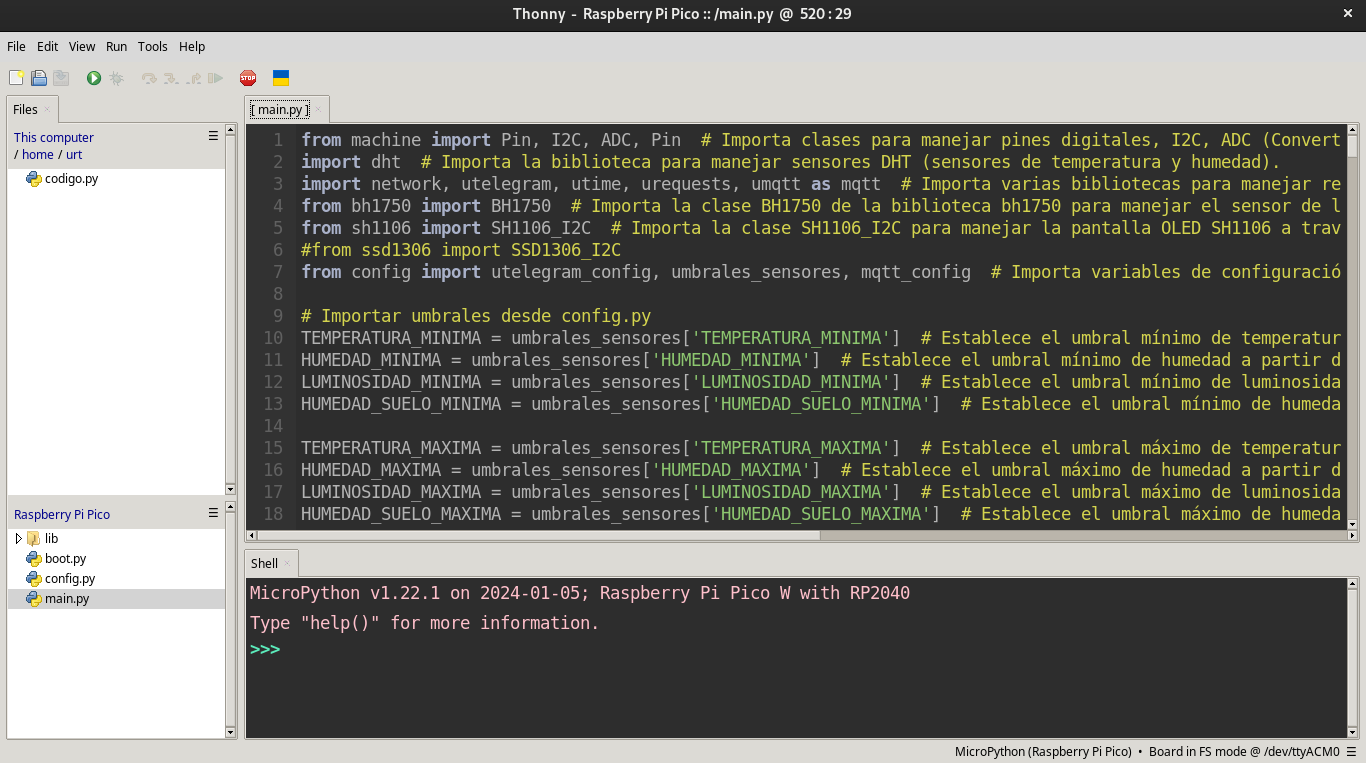
\includegraphics[width=1\textwidth]{img/herramientas/thonny.png}
    \caption{IDE Thonny.} \label{Img:Thonny}
\end{figure}
 \pagebreak

\subsection{Entorno de desarrollo Python}\label{4:Python}
\begin{itemize}
    \item \textbf{Herramientas valoradas:} \href{https://colab.google/}{Google colab} y \href{https://jupyter.org/}{Jupyter Notebook}.
    \item \textbf{Herramienta elegida:} \href{https://jupyter.org/}{Jupyter Notebook}.
\end{itemize}

Jupyter Notebook~\cite{misc:Jupyter_Notebook} es una herramienta de código abierto poderosa que facilita la creación y compartición de documentos interactivos. Estos documentos pueden contener código ejecutable, visualizaciones, texto narrativo y otros elementos. Opto por utilizar Jupyter Notebook en mi Trabajo de Fin de Grado debido a su versatilidad y capacidad para aprovechar los entornos virtuales que he configurado en mi computadora. Este entorno se ha vuelto fundamental para llevar a cabo análisis de datos, especialmente haciendo uso intensivo de la biblioteca Pandas~\cite{misc:Pandas} para manipulación y procesamiento de datos.
%\begin{figure}[h]
    %\centering
    %
\includegraphics[width=0.1\textwidth]{img/herramientas/jupyter_logo.png}
    %\caption{Jupyter logo.} \label{Img:Jupyter}
%\end{figure}
\pagebreak
\section{Control de datos}
\subsection{APIS}\label{4:APIS}
\begin{itemize}
    \item \textbf{API de Telegram:}
La API de Telegram~\cite{misc:Telegram_api}, accesible a través de la URL \url{https://api.telegram.org/bot<token>}, juega un papel fundamental en la integración de bots de Telegram~\cite{misc:Telegram_bots} con el sistema. Permite la interacción bidireccional entre el sistema y los usuarios a través de la plataforma de mensajería Telegram. Al utilizar esta API, se establece una conexión segura para enviar y recibir mensajes, comandos y datos entre el sistema y los usuarios mediante la implementación de funciones específicas proporcionadas por Telegram. Esto posibilita la notificación remota, la recopilación de datos y la activación de acciones automatizadas, contribuyendo así a la funcionalidad integral del sistema de control de datos.
Esta API fue usada en el código MicroPython.
    \item \textbf{API WorldTime}\label{4:API_Hora}
		La API de WorldTime~\cite{misc:WorlTimeAPI}, accesible mediante la URL \url{http://worldtimeapi.org/api/ip}, ofrece información precisa sobre la hora mundial basada en la ubicación asociada a la dirección IP del usuario. Al realizar una solicitud a esta API, se obtiene información detallada sobre la hora actual, la fecha, el huso horario y otros datos relacionados con la hora en la ubicación correspondiente a la dirección IP consultada. Esta API es valiosa para aplicaciones que requieren sincronización horaria precisa y la visualización de la hora actual en diferentes regiones del mundo. Su facilidad de acceso y respuesta estructurada la convierten en una herramienta útil para integrar la información horaria global en aplicaciones y sistemas.
Esta API fue usada en el código MicroPython.
\end{itemize}
\pagebreak

\section{Entorno Hardware}
\subsection{Fritzing}
Fritzing~\cite{misc:Fritzing} es una herramienta de diseño electrónico de código abierto que facilita la creación de esquemas, prototipos y layouts de placas de circuito impreso (PCB). Diseñado para usuarios, desde principiantes hasta expertos, Fritzing ofrece una interfaz intuitiva y gráfica que permite la conexión visual de componentes electrónicos, como sensores, actuadores y placas de desarrollo. Su funcionalidad principal abarca desde la creación de esquemas eléctricos hasta la generación de archivos Gerber para la fabricación de PCB. Fritzing se destaca por su accesibilidad y capacidad para convertir conceptos de diseño en proyectos electrónicos tangibles, lo que lo convierte en una herramienta valiosa para ingenieros, diseñadores y entusiastas que desean visualizar y materializar sus ideas electrónicas.
\begin{figure}[h]
    \centering
    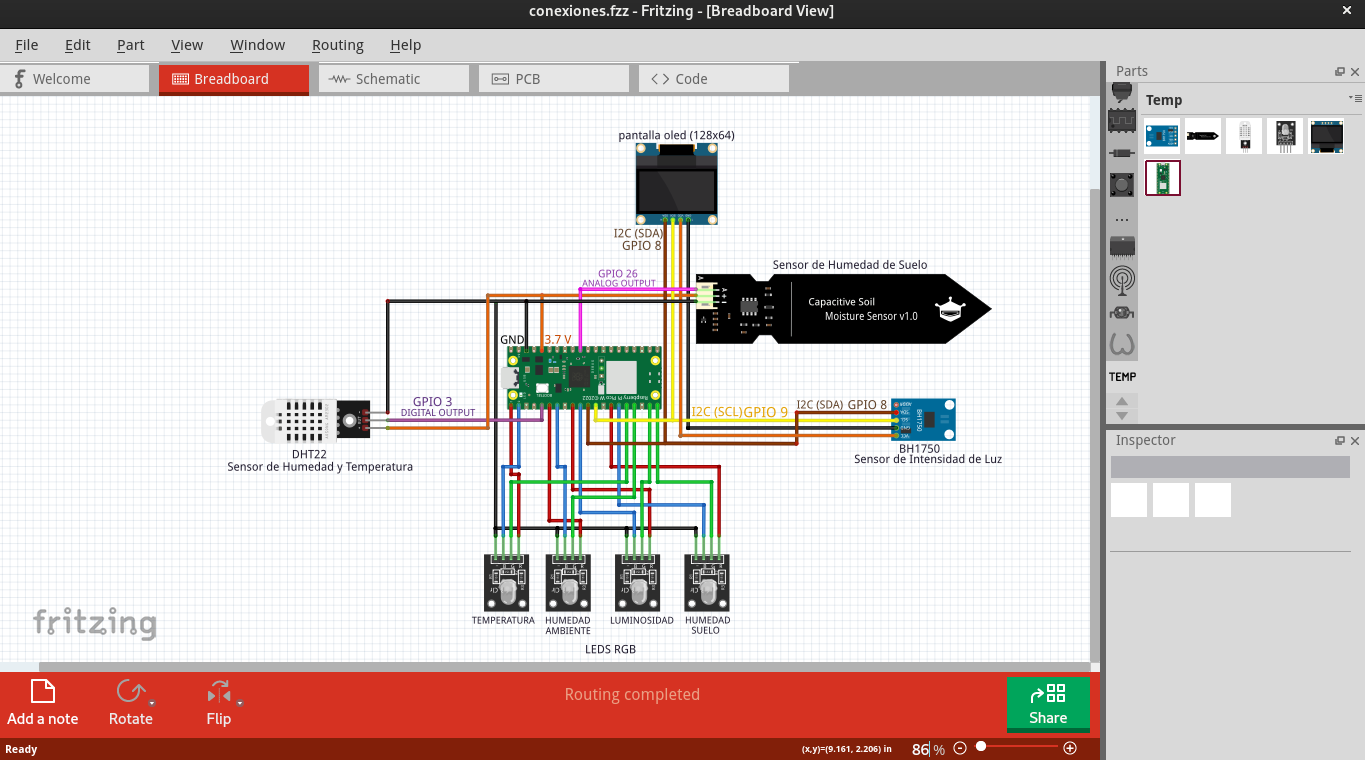
\includegraphics[width=1\textwidth]{img/herramientas/fritzing.png}
    \caption{Esquema de conexiones diseñado con Fritzing.}
\end{figure}
\pagebreak

\section{Metodologías}
\subsection{Modelo de prototipos}
El modelo de prototipos~\cite{misc:Metodologia_ModeloDePrototipos} es una metodología de desarrollo de software que se centra en la creación temprana y rápida de versiones simplificadas de un sistema para obtener retroalimentación y comprensión de los requisitos del usuario. En lugar de esperar hasta la fase final del desarrollo para presentar un producto completo, el enfoque de prototipos permite construir versiones iterativas y evolutivas del sistema.

El proceso típico del modelo de prototipos implica las siguientes etapas:
\begin{itemize}
	\item \textbf{Definición de Requisitos:}
Se identifican y documentan los requisitos iniciales del sistema.

\item \textbf{Desarrollo del Prototipo:}
Se construye un prototipo inicial que representa visualmente las funcionalidades clave del sistema.

\item \textbf{Evaluación y Retroalimentación:}
Los usuarios y las partes interesadas evalúan el prototipo y proporcionan retroalimentación sobre su diseño y funcionalidad.

\item \textbf{Refinamiento Iterativo:}
Con base en la retroalimentación recibida, se realizan ajustes y mejoras en el prototipo, creando iteraciones sucesivas.

\item \textbf{Validación de Requisitos:}
La validación continua de los prototipos ayuda a refinar y validar los requisitos del sistema a lo largo del proceso.
\end{itemize}

Este enfoque iterativo y colaborativo permite una mayor flexibilidad en la adaptación a cambios en los requisitos del usuario y facilita la comunicación entre los desarrolladores y los stakeholders. El modelo de prototipos es particularmente útil en situaciones donde los requisitos no están completamente claros desde el principio o cuando se busca una comprensión más profunda de las necesidades del usuario antes de la implementación final del sistema.

\subsection{Metodología cascada}
La metodología cascada~\cite{misc:Metodologia_Cascada}, también conocida como el modelo de desarrollo en cascada, es una metodología de desarrollo de software que sigue un enfoque lineal y secuencial. Aunque ha sido utilizada en proyectos de software en el pasado, en la actualidad se considera menos flexible y adaptable en comparación con metodologías más modernas y ágiles.
En el modelo cascada, el proceso de desarrollo sigue una secuencia fija de fases, que generalmente incluyen:

\begin{enumerate}
\item Requisitos
\item Diseño
\item Implementación
\item Pruebas
\item Despliegue
\item Mantenimiento
\end{enumerate}

Cada fase depende de la finalización exitosa de la fase anterior, y los cambios en las etapas posteriores pueden ser difíciles y costosos de implementar una vez que el proyecto ha avanzado. Este enfoque puede no ser el más adecuado para proyectos donde los requisitos pueden cambiar con frecuencia o donde la adaptabilidad es esencial.

En muchos proyectos actuales, especialmente en el ámbito académico, se prefiere el uso de metodologías más ágiles y flexibles, como Scrum, Kanban o el enfoque de desarrollo iterativo e incremental.

En conclusión, aunque la metodología cascada ha sido utilizada en el pasado, hoy en día muchas organizaciones y proyectos prefieren metodologías más ágiles y adaptables. La elección de la metodología dependerá de los requisitos y características específicas de cada proyecto de TFG.

\section{Entorno de desarrollo del Proyecto}
\subsection{Control de versiones o CVS, Concurrent Versioning System}\label{4:controlVersiones}
\begin{itemize}
    \item \textbf{Herramientas valoradas:} \href{https://git-scm.com/}{Git}, \href{https://subversion.apache.org/}{SVN}.
    \item \textbf{Herramienta elegida:} \href{https://git-scm.com/}{Git}.
\end{itemize}
Git~\cite{misc:Git} es un sistema de control de versiones distribuido, ampliamente utilizado en el desarrollo de software y es conocido por su velocidad, flexibilidad y eficiencia en la gestión de versiones de código fuente.

Comparación con SVN:

Subversion (SVN)~\cite{misc:SVN} es otro sistema de control de versiones, pero sigue un modelo centralizado, a diferencia del modelo distribuido de Git. Aquí hay algunas diferencias clave y ventajas de Git sobre SVN:
\begin{itemize}
	\item \textbf{Descentralización:}
Git es completamente descentralizado, lo que significa que cada usuario tiene una copia completa del repositorio con todo su historial. En SVN, los usuarios dependen del servidor central para muchas operaciones.

\item \textbf{Ramificación y Fusiones Rápidas:}
Git permite ramificaciones ligeras y fusiones rápidas, lo que facilita el desarrollo paralelo y la gestión de características en diferentes ramas. SVN maneja ramificaciones y fusiones, pero históricamente ha sido menos eficiente en comparación con Git.

\item \textbf{Eficiencia en Red:}
Git es más eficiente en términos de ancho de banda y operaciones de red, ya que las operaciones se realizan localmente en la mayoría de los casos. SVN, al depender más del servidor central, puede ser más lento en operaciones que implican la red.

\item \textbf{Historial Completo y Offline:}
Git almacena el historial completo localmente, lo que permite el trabajo fuera de línea. SVN requiere acceso al servidor para recuperar el historial completo.

\item \textbf{Flexibilidad y Escalabilidad:}
Git es conocido por su flexibilidad y escalabilidad, especialmente en proyectos grandes y complejos. SVN puede encontrar limitaciones en proyectos extensos y complejos.
\end{itemize}


\subsection{Hosting del Repositorio}
\begin{itemize}
    \item \textbf{Herramientas valoradas:} \href{https://github.com/}{Github} y \href{https://bitbucket.org/product/}{Bitbucket}.
    \item \textbf{Herramienta elegida:} \href{https://github.com/}{Github}.
\end{itemize}
GitHub~\cite{misc:Github} es una plataforma de desarrollo colaborativo basada en Git que facilita el alojamiento y la colaboración en proyectos de software. 

Bitbucket~\cite{misc:Bitbucket} es otra plataforma de desarrollo colaborativo basada en Git, pero hay algunas diferencias clave. Aquí se exploran estas diferencias y se destaca una ventaja de GitHub sobre Bitbucket:

\begin{itemize}
	\item \textbf{Visibilidad del Código Fuente:}
		GitHub ha sido históricamente más popular para proyectos de código abierto, y los repositorios públicos en GitHub suelen tener una mayor visibilidad y participación de la comunidad en comparación con Bitbucket.

\item \textbf{Comunidad y Desarrollo Abierto:}
GitHub se ha convertido en el estándar de facto para proyectos de código abierto, y muchos desarrolladores buscan activamente proyectos en GitHub. Esto hace que sea más fácil para los proyectos atraer colaboradores y contribuyentes.

\item \textbf{Integraciones y Ecosistema:}
GitHub tiene una amplia gama de integraciones y herramientas de terceros que son ampliamente utilizadas en la comunidad de desarrollo. La rica integración con servicios como Travis CI, CircleCI y otros facilita el desarrollo y la automatización.

\item \textbf{Herramientas de Colaboración:}
Mientras que Bitbucket ofrece características similares, GitHub es generalmente preferido por su interfaz de usuario intuitiva, herramientas de revisión de código más robustas y una experiencia general más pulida para la colaboración.

\item \textbf{Repositorios Públicos Gratuitos:}
GitHub permite la creación de repositorios públicos de forma gratuita, lo que fomenta la participación y el desarrollo colaborativo en proyectos de código abierto. Bitbucket, por otro lado, suele ofrecer repositorios privados gratuitos, pero limita la cantidad de colaboradores.
\end{itemize}


\subsection{Editor del proyecto}\label{4:ATOM}
\begin{itemize}
    \item \textbf{Herramientas valoradas:} \href{https://www.vim.org/}{VIM}, \href{https://code.visualstudio.com/}{Visual Studio Code}, \href{https://www.sublimetext.com/}{Sublime}.
    \item \textbf{Herramienta elegida:} \href{https://code.visualstudio.com/}{Visual Studio Code}.
\end{itemize}

\subsection{Dibujos, diagramas y planos}\label{4:plataformasDibujosYPlanos}

\begin{itemize}
	\item \textbf{Herramientas valoradas:} \href{https://inkscape.org/}{Inkscape}, \href{https://www.gimp.org/}{GIMP}, \href{https://support.microsoft.com/es-es/windows/obtener-microsoft-paint-a6b9578c-ed1c-5b09-0699-4ed8115f9aa9}{Paint, Paint3D}, \href{https://www.adobe.com/es/products/photoshop.html}{Photoshop}, y \href{www.draw.io}{Draw.io}.
	\item \textbf{Herramienta elegida:} \href{https://www.gimp.org/}{GIMP} y \href{https://www.adobe.com/es/products/photoshop.html}{Photoshop}.
\end{itemize}


\subsection{Procesador de textos \LaTeX}\label{4:latex}
\begin{itemize}
    \item \textbf{Herramientas valoradas:} \href{https://www.latex-project.org/}{\LaTeX}, \href{https://www.microsoft.com/es-es/microsoft-365/word}{MS Word}, \href{https://www.sublimetext.com/}{Sublime}, \href{https://www.overleaf.com/}{Overleaf}.
    \item \textbf{Herramienta elegida:} \href{https://www.latex-project.org/}{\LaTeX} y \href{https://www.overleaf.com/}{Overleaf}.
\end{itemize}
\LaTeX{}~\cite{misc:Latex} es un sistema de preparación de documentos que se utiliza ampliamente para la creación de documentos científicos, técnicos y académicos. A diferencia de los procesadores de texto tradicionales, LaTeX se basa en la creación de documentos mediante instrucciones de marcado en lugar de formatos visuales directos. Los usuarios escriben el contenido del documento junto con comandos LaTeX que definen la estructura, el formato y otros elementos.

Overleaf~\cite{misc:Overleaf} es una plataforma en línea que permite la colaboración en tiempo real y la edición de documentos LaTeX. Algunas razones para considerar el uso de Overleaf junto con LaTeX son:
\begin{itemize}
	\item \textbf{Colaboración en Tiempo Real:}
Overleaf facilita la colaboración en documentos LaTeX entre múltiples autores en tiempo real, permitiendo que varios colaboradores trabajen simultáneamente en un proyecto.

\item \textbf{Entorno en Línea:}
No es necesario instalar LaTeX localmente en tu máquina. Overleaf proporciona un entorno en línea que elimina la necesidad de configurar y mantener un sistema LaTeX en tu computadora.

\item \textbf{Plantillas y Recursos:}
Overleaf ofrece una variedad de plantillas predefinidas para diferentes tipos de documentos, lo que facilita el inicio de nuevos proyectos. Además, proporciona acceso a una amplia variedad de recursos y tutoriales.

\item \textbf{Control de Versiones Integrado:}
Overleaf tiene un sistema de control de versiones integrado que permite realizar un seguimiento de los cambios en el documento y revertir a versiones anteriores si es necesario.

\item \textbf{Exportación y Publicación:}
Overleaf permite exportar documentos a diferentes formatos (PDF, HTML, etc.) y facilita la publicación directa en revistas académicas que admiten el formato LaTeX.
\end{itemize}
\pagebreak

\subsection{Calidad del Código}
\begin{itemize}
	\item \textbf{Herramientas valoradas:} \href{https://www.sonarsource.com/products/sonarcloud/}{SonarCloud}, \href{https://codebeat.co/}{Codebeat}, \href{https://www.codacy.com/}{Codacy} y \href{https://www.sonarsource.com/products/sonarqube/}{SonarQube}.
    \item \textbf{Herramienta elegida:} \href{https://www.sonarsource.com/products/sonarcloud/}{SonarCloud}.
\end{itemize}
SonarCloud~\cite{misc:SonarCloud}, elegido para optimizar la calidad del código en mi proyecto, realiza revisiones exhaustivas en la nube y ofrece valiosas sugerencias para mejorar. Su integración en tiempo real con GitHub asegura una evaluación continua y facilita la corrección de problemas de código de manera inmediata. 

\section{Entorno físico}
\subsection{Raspberry Pi Pico W}
La Raspberry Pi Pico W~\cite{manual:RPiPicoW_datasheet} es un microcontrolador de bajo costo y alto rendimiento desarrollado por la Fundación Raspberry Pi. Se basa en el chip RP2040 diseñado por Raspberry Pi, que integra un procesador ARM Cortex-M0+ de doble núcleo y ofrece una serie de características diseñadas para proyectos de electrónica y programación embebida.

\begin{table}[htbp]
\begin{center}
\caption{Características de la Raspberry Pi Pico W.}
\begin{tabular}{|l|l|}
\hline
\rowcolor[HTML]{C0C0C0} 
\textbf{Característica} & \textbf{Descripción}\\ \hline
Microcontroller	& RP2040 @ 133MHz, 264kB SRAM \\ \hline
Procesador & Dual Core ARM Cortex-M0+ \\ \hline
Flash memory &	2MB \\ \hline
Exposed GPIO & 26 \\ \hline
ADC	& 3 channels \\ \hline
I2C	& 2 \\ \hline
SPI	& 2 \\ \hline
UART & 2 \\ \hline
PWM	& 16 channels	 \\ \hline
Wireless interfaces & Wifi 802.11n, Bluetooth 5.2\\ \hline
\end{tabular}
\end{center}
\end{table}
\pagebreak

\begin{figure}[h]
    \centering
    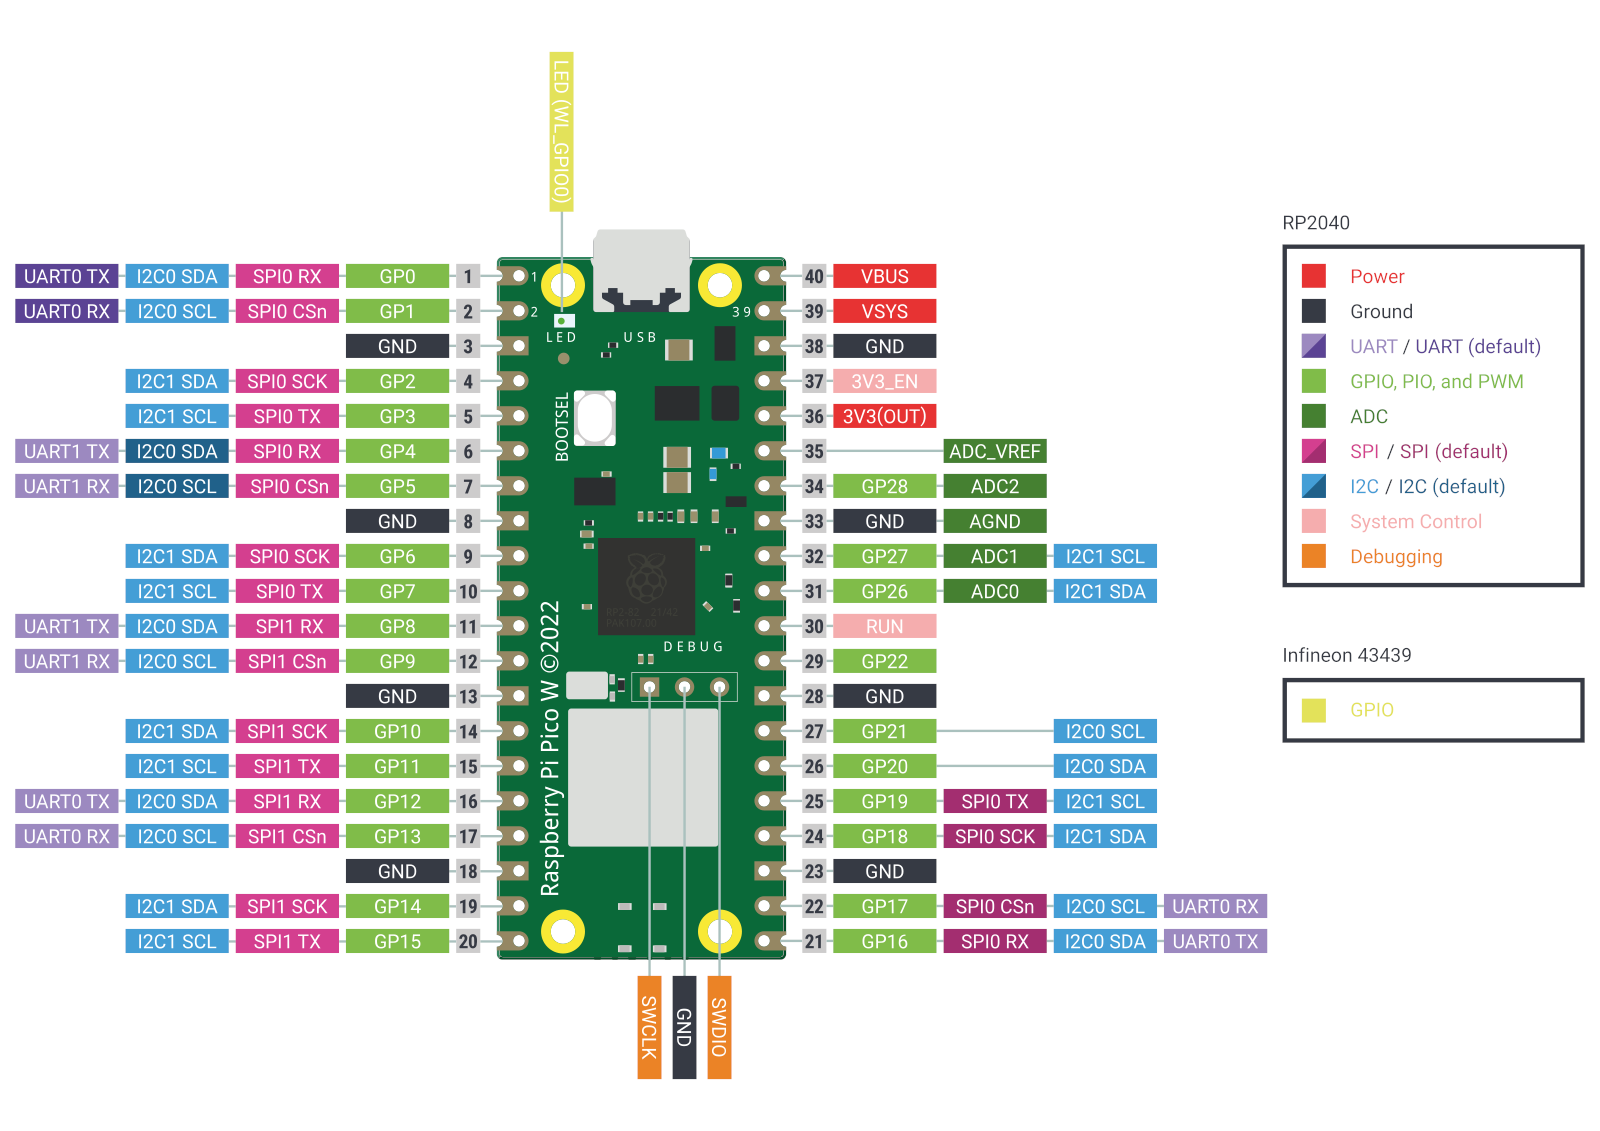
\includegraphics[width=1\textwidth]{img/herramientas/picow.png}
    \caption{Raspberry Pi Pico W Pinout.}
\end{figure}

\begin{figure}[h]
    \centering
    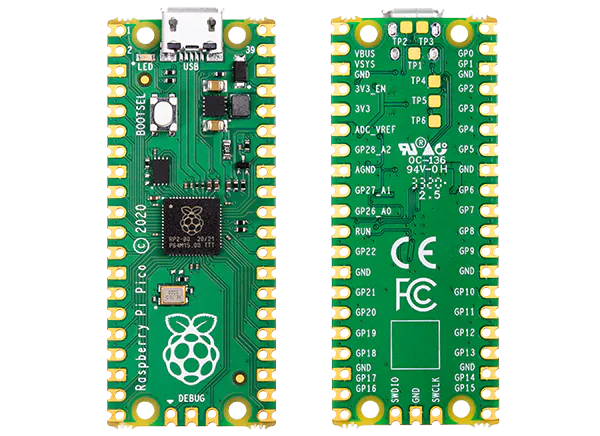
\includegraphics[width=0.5\textwidth]{img/herramientas/picow_vistas.png}
    \caption{Vistas Frontal y posterior de Raspberry Pi Pico W.}
\end{figure}

\pagebreak

\subsection{Pantalla oled I2C de 128x64 píxeles y 1.3 pulgadas}
La pantalla OLED~\cite{manual:Oled} de 128x64 de 1.3 pulgadas con interfaz I2C es un dispositivo de visualización que utiliza la tecnología OLED (Diodo Orgánico de Emisión de Luz) y se comunica a través del protocolo I2C (Inter-Integrated Circuit).

\begin{table}[htbp]
\begin{center}
\caption{Características de la pantalla oled}
\begin{tabular}{|l|l|}
\hline
\rowcolor[HTML]{C0C0C0} 
\textbf{Característica} & \textbf{Descripción}\\ \hline
Voltaje de operación & 3V\quad-\quad5.5 V DC\\ \hline
Interfaz & I2C\\ \hline
Resolución & 128\times64\\ \hline
Monócromo & píxeles blancos (fondo negro)\\ \hline
Ángulo de visión & 160^\circ \\ \hline
Área visicle (display) & 23$\times$11.5 mm\\ \hline
Consumo de energía ultra bajo & 0.08 W (cuando están encendidos todos los píxeles)\\ \hline
item Temperatura de trabajo & -30\textcelsius\quad -\quad70\textcelsius \\ \hline
item Dimensiones & 27\times 27$\times$4.1mm \\ \hline
item Peso & 5 gramos \\ \hline
\end{tabular}
\end{center}
\end{table}

\begin{figure}[h]
    \centering
    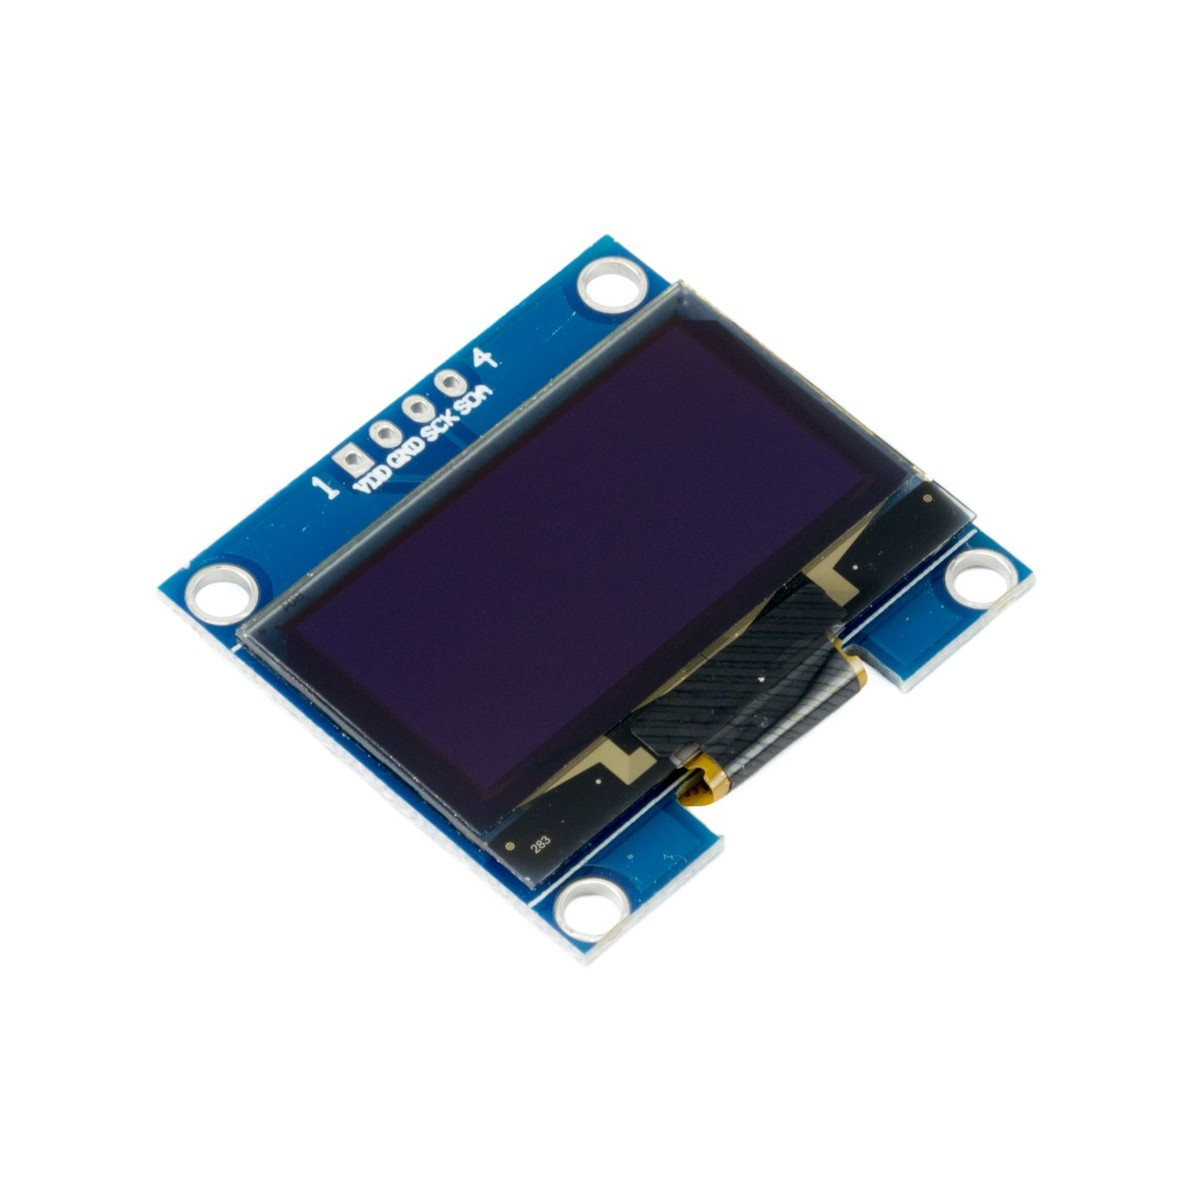
\includegraphics[width=0.5\textwidth]{img/herramientas/oled_cara.png}
    \caption{Pantalla oled.}
\end{figure}

%\begin{figure}[h]
    %\centering
    %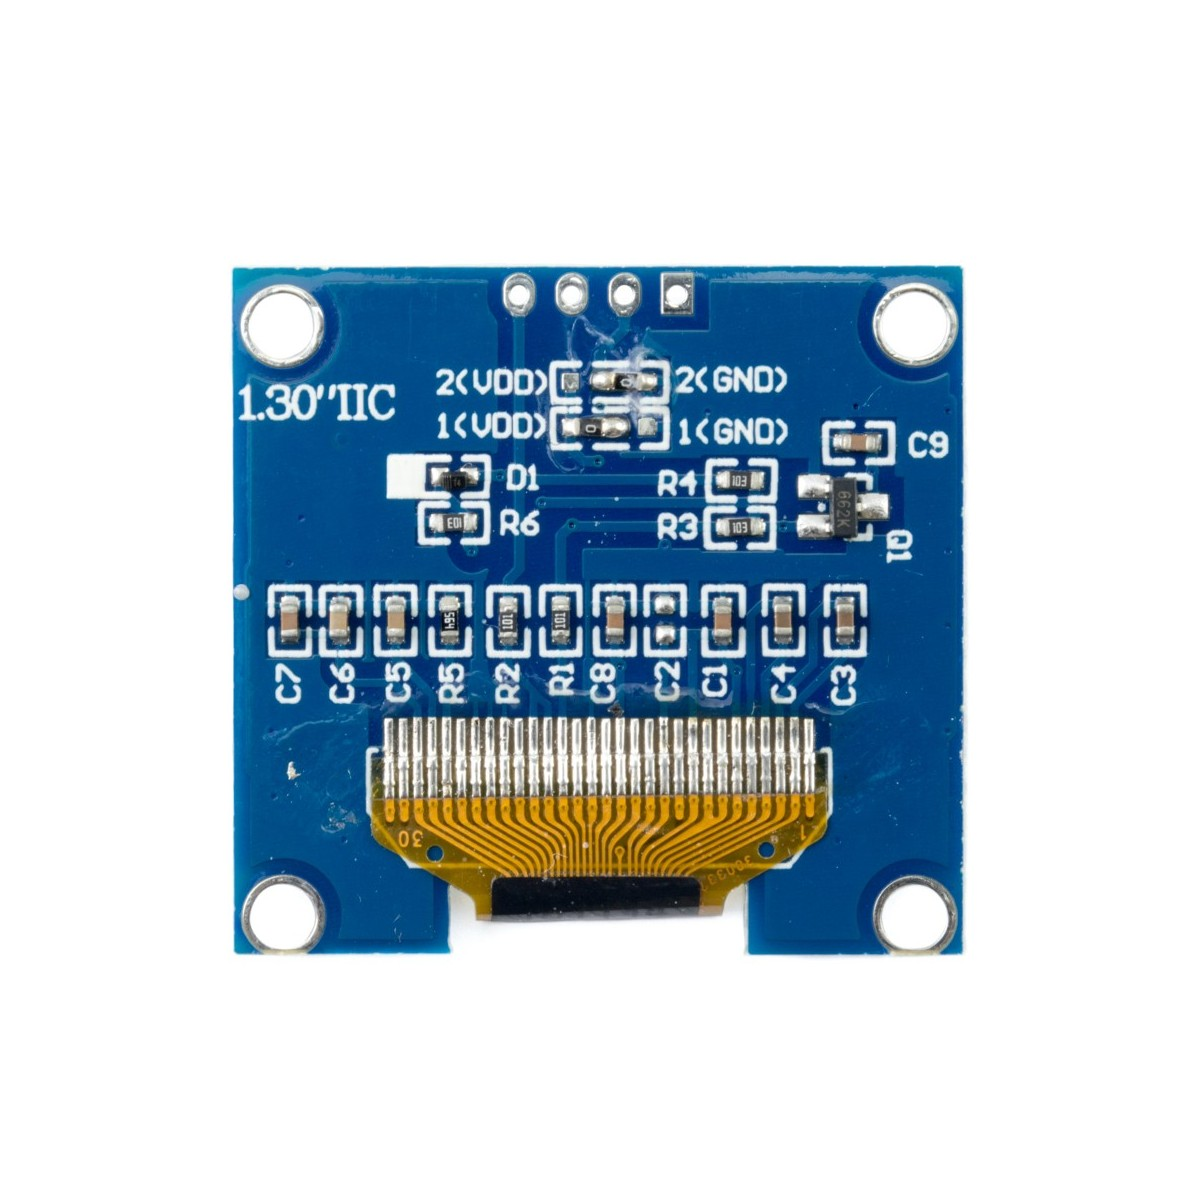
\includegraphics[width=0.5\textwidth]{img/herramientas/oled_reverso.png}
    %\caption{Vista posterior de la pantalla oled.}
%\end{figure}
\pagebreak

\subsection{Sensor de luz BH1750}

El sensor BH1750~\cite{manual:BH1750} es un sensor de intensidad de luz digital que mide la luminosidad ambiental en lux (lx). Este dispositivo es utilizado comúnmente en aplicaciones donde se requiere monitoreo de la luz, como en sistemas de iluminación automática, dispositivos de ahorro de energía y proyectos de IoT.
Posee un conversor interno de 16-bit, por lo que entrega una salida digital en formato I2C

\begin{table}[htbp]
\begin{center}
\caption{Características del sensor de luz BH1750.}
\begin{tabular}{|l|l|}
\hline
\rowcolor[HTML]{C0C0C0} 
\textbf{Característica} & \textbf{Descripción}\\ \hline
Voltaje de Operación &  3V – 5V \\ \hline
Interfaz digital & I2C \\ \hline
Respuesta espectral & similar a la del ojo humano \\ \hline
Rango de medición & 1 lux\quad-\quad65535 lux \\ \hline
Consumo de energía & bajo \\ \hline
\end{tabular}
\end{center}
\end{table}

\begin{figure}[h]
    \centering
    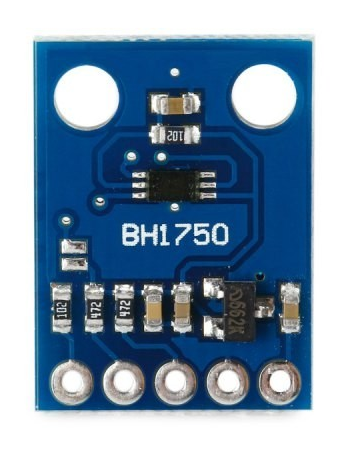
\includegraphics[width=0.4\textwidth]{img/herramientas/bh1750_cara.png}
    \caption{Vista frontal del sensor BH1750.}
\end{figure}
\pagebreak

\begin{figure}[h]
    \centering
    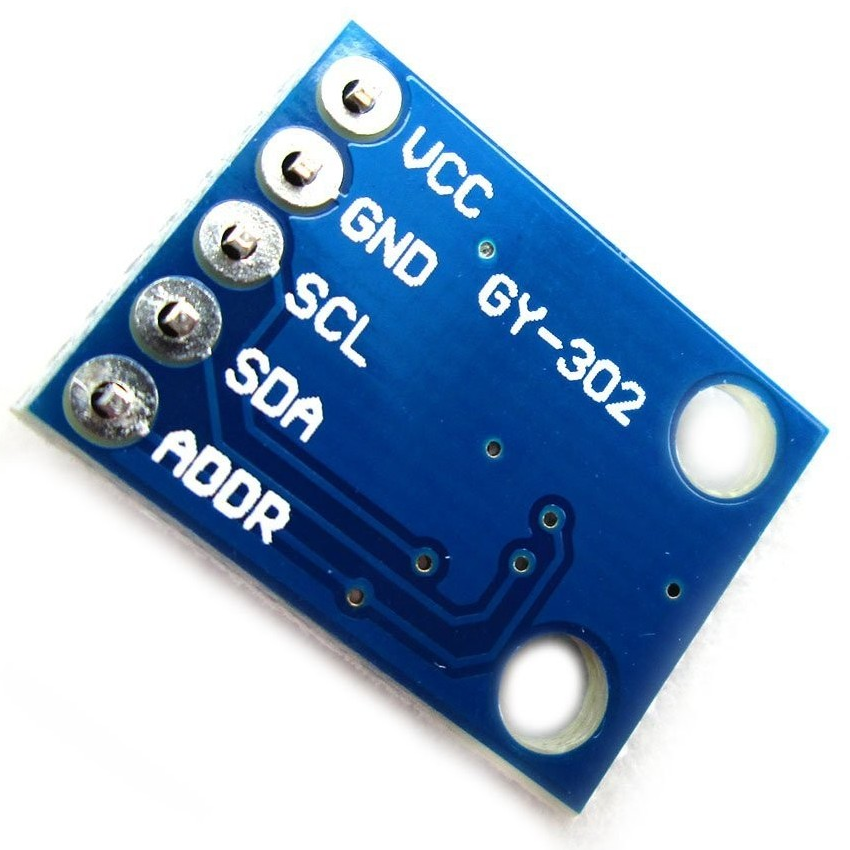
\includegraphics[width=0.4\textwidth]{img/herramientas/bh1750_reverso.png}
    \caption{Lado posterior del sensor BH1750.}
\end{figure}
\pagebreak

\subsection{Sensor de temperatura y humedad DHT22}
El sensor DHT22~\cite{manual:DHT22} (también conocido como AM2302) es un sensor de temperatura y humedad digital utilizado en aplicaciones donde es crucial monitorear y medir las condiciones ambientales.

\begin{table}[htbp]
\begin{center}
\caption{Características del sensor de temperatura y humedad DHT22.}
\begin{tabular}{|l|l|}
\hline
\rowcolor[HTML]{C0C0C0} 
\textbf{Característica} & \textbf{Descripción}\\ \hline
Voltaje de funcionamiento &  3 V\quad-\quad 5.5 V \\ \hline
Forma de salida de señal & señal digital \\ \hline
Rango de medición de temperatura & -40 \textcelsius\quad -\quad 80 \textcelsius  \\ \hline
Rango de medición de humedad & 0\quad-\quad100\% HR \\ \hline
Resolución de temperatura & 0.1 \textcelsius \\ \hline
Resolución de humedad & 0.1\% HR \\ \hline
Precisión de medición de temperatura & $\pm$0.5 \textcelsius \\ \hline
Precisión de medición de humedad & \pm 2$\%$ $ HR$ \\ \hline
Tamaño & 28.2 x 13.1 x 10 mm \\ \hline
Tiempo de sensado & 2s \\ \hline
Modelo & AM2302 \\ \hline
\end{tabular}
\end{center}
\end{table}
\begin{figure}[h]
    \centering
    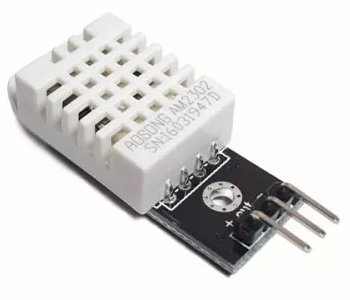
\includegraphics[width=0.7\textwidth]{img/herramientas/dht22.png}
    \caption{Sensor DHT22.}
\end{figure}

\subsection{Sensor de humedad de suelo}
El sensor de humedad de suelo Higrometro V1.2~\cite{wiki:SensorHumedadSuelo} es un dispositivo diseñado para medir la humedad del suelo en entornos agrícolas, de jardinería u otros contextos donde el control de la humedad del suelo es esencial.

\begin{table}[htbp]
\begin{center}
\caption{Características del sensor de humedad de suelo.}
\begin{tabular}{|l|l|}
\hline
\rowcolor[HTML]{C0C0C0} 
\textbf{Característica} & \textbf{Descripción}\\ \hline
Voltaje de alimentación & 3.3V\quad-\quad5V DC \\ \hline
Corriente operación & 5 mA \\ \hline
Voltaje de la señal de salida & 0 a 5V (Analógico) \\ \hline
Modelo & capacitive soil moisture sensor v1.2 \\ \hline
Vida útil & 3 años mínimo \\ \hline
Conector & PH2.0-3P \\ \hline
Dimensiones & 98$\times$23 mm \\ \hline
Peso & 15 gramos \\ \hline
\end{tabular}
\end{center}
\end{table}

\begin{figure}[h]
    \centering
    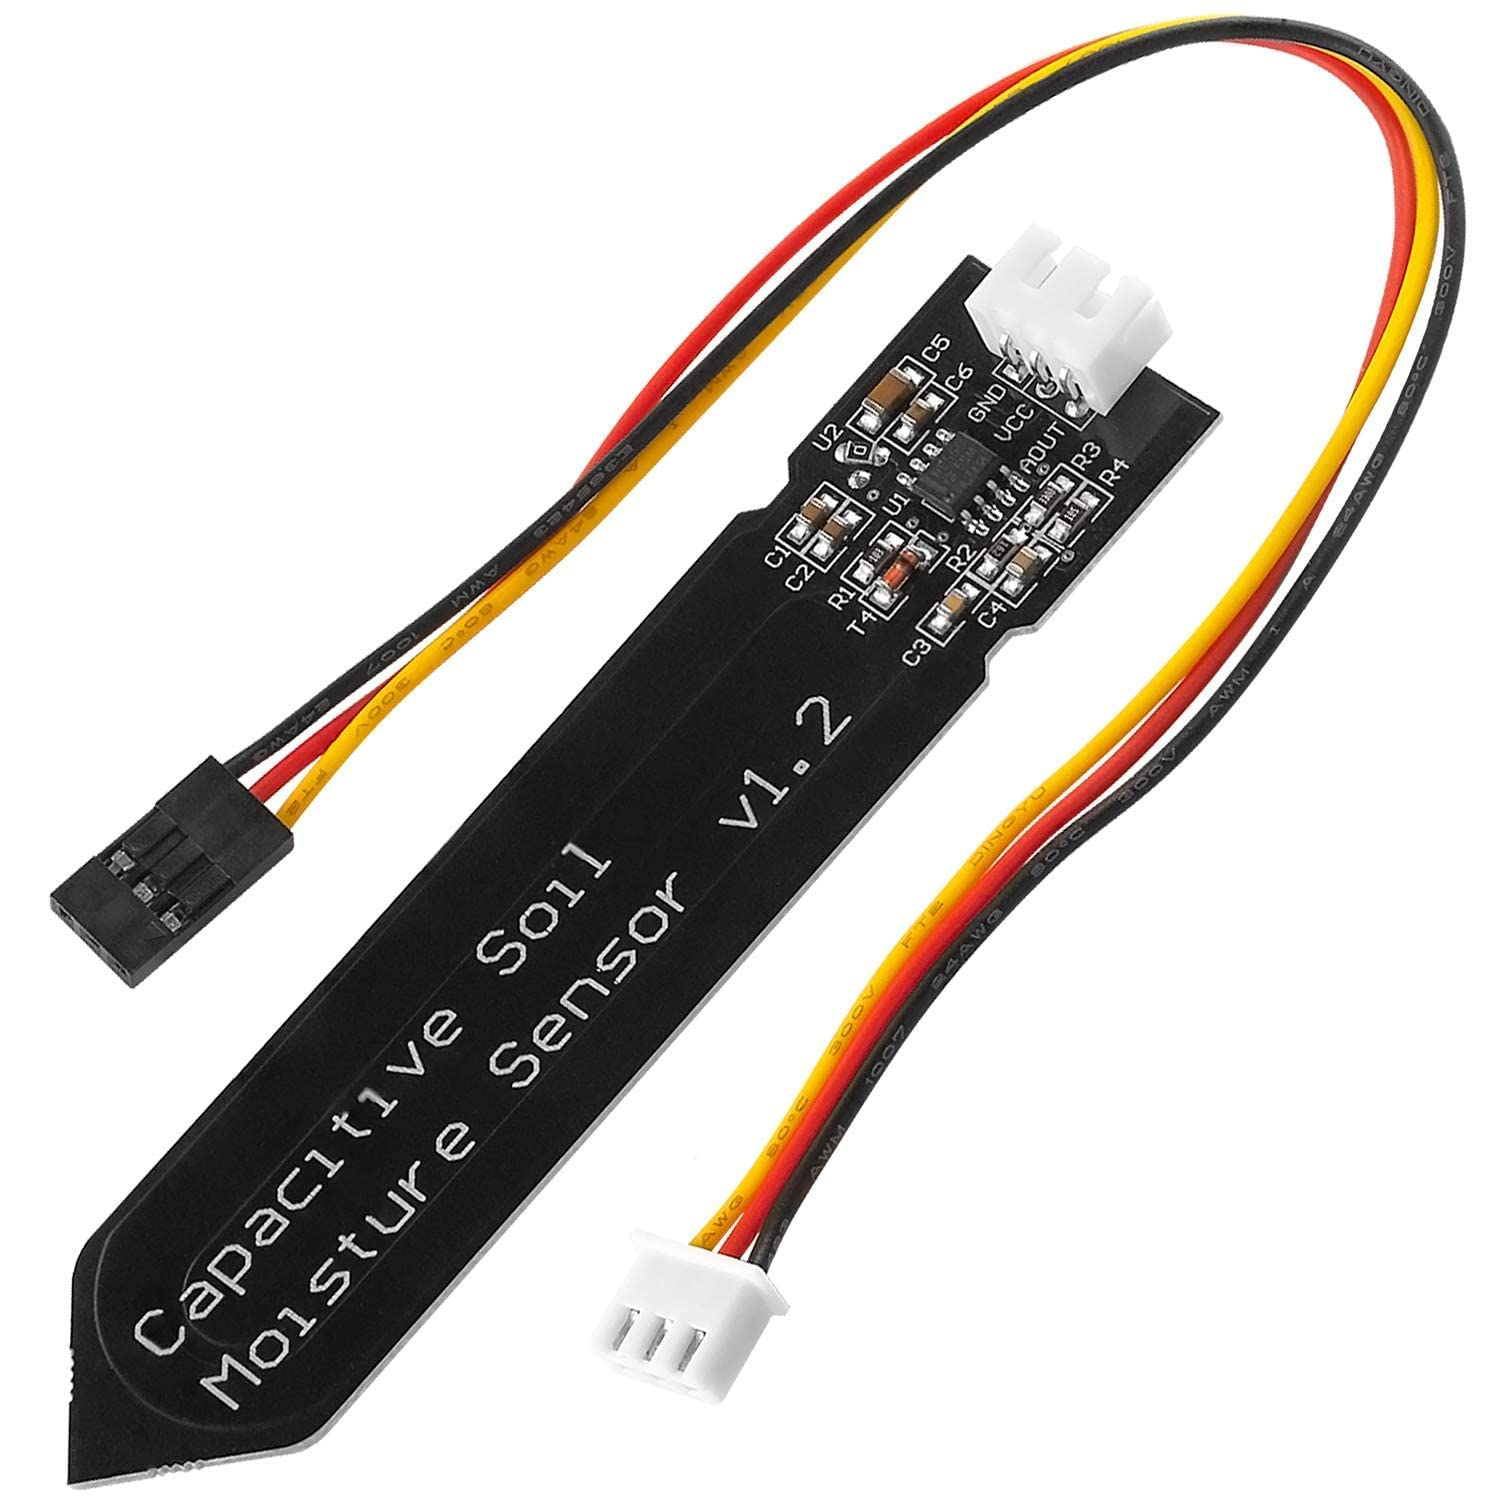
\includegraphics[width=0.7\textwidth]{img/herramientas/SensorHumedadSuelo.png}
    \caption{Sensor de humedad de suelo Higrometro V1.2.}
\end{figure}

\subsection{KY-016 FZ0455 Módulo led RGB de 3 colores}
El módulo KY-016~\cite{manual:LedRGB} FZ0455 es un dispositivo electrónico que contiene un LED RGB (Light Emitting Diode - Diodo Emisor de Luz) capaz de emitir luz en tres colores primarios: rojo, verde y azul. Este módulo se utiliza comúnmente en proyectos electrónicos y de iluminación para agregar efectos de luz y color controlables

\begin{table}[htbp]
\begin{center}
\caption{Características del módulo led RGB KY-016.}
\begin{tabular}{|l|l|} %|c|c|
\hline
\rowcolor[HTML]{C0C0C0} 
\textbf{Característica} & \textbf{Descripción}\\ \hline
Voltaje operativo & 3.3 V\quad5 V\\ \hline
Modo de accionamiento led & Accionamiento de cátodo común \\ \hline
Tamaño & 3.5$\times$0.8 cm\\ \hline
Voltaje de avance V_{f}[Red] & 1.8 V \\ \hline
Voltaje de avance V_{f}[Green, Blue] & 2.8 V \\ \hline
Corriente directa hacia adelante I_{f} & 20 mA \\ \hline
\end{tabular}
\end{center}
\end{table}

\begin{figure}[h]
    \centering
    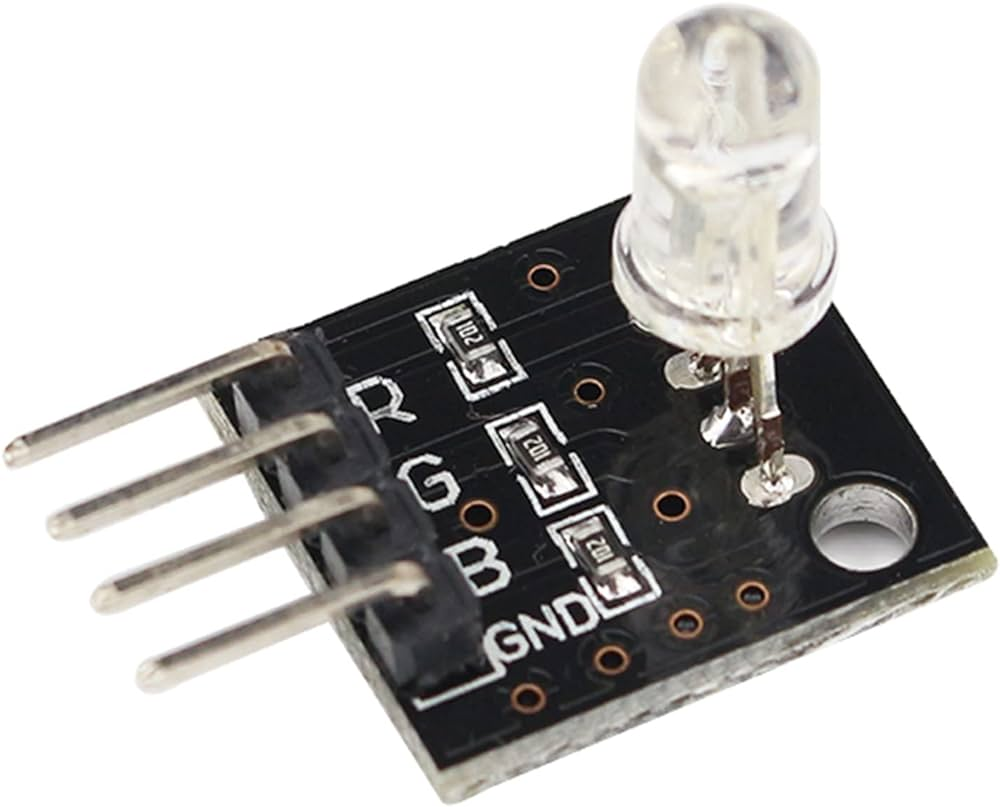
\includegraphics[width=0.8\textwidth]{img/herramientas/LedRGB.png}
    \caption{Módulo led RGB KY-016.} \label{Img:LedRGB}
\end{figure}

\subsection{Enrutador WiFi USB 4G LTE}
El Enrutador WiFi~\cite{misc:EnrutadorWifi} USB 4G LTE es un dispositivo portátil que permite establecer una conexión a Internet de alta velocidad utilizando la red móvil 4G LTE. Diseñado para la movilidad y la conveniencia, este router WiFi ofrece una solución eficiente para aquellos que requieren acceso a la red en cualquier lugar donde haya cobertura de red móvil. Con una ranura para tarjeta SIM, el dispositivo facilita la inserción de una tarjeta SIM compatible, lo que lo convierte en una opción versátil para la conectividad a Internet en movimiento. Con una velocidad de transferencia de hasta 150 Mbps, este enrutador proporciona un rendimiento adecuado para actividades en línea como navegación web, transmisión de video y juegos en línea.

\begin{table}[htbp]
\begin{center}
\caption{Características del enrutador WiFi USB 4G LTE.}
\begin{tabular}{|l|l|}
\hline
\rowcolor[HTML]{C0C0C0} 
\textbf{Característica} & \textbf{Descripción}\\ \hline
Velocidad de Transferencia &  Hasta 150 Mbps\\ \hline
Red Móvil Compatible &  Tecnología 4G LTE \\ \hline
4G LTE FDD & B1/B3/B5 \\ \hline
Wifi & Support IEEE802.11b/g/n Band 2.4G \\ \hline
Número máximo de usuarios & 10 \\ \hline
Ranura para Tarjeta SIM &  Necesario para la conexión a la red móvil \\ \hline
Conectividad WiFi & Proporciona una red WiFi local\\ \hline
Compatibilidad & Computadoras, tabletas y teléfonos \\ \hline
Seguridad & Cifrado WPA/WPA2 \\ \hline
Alimentación por batería & Es opcional y permite mayor portabilidad \\ \hline
Indicadores LED & Estado de la conexión e intensidad de la señal \\ \hline
Material & ABS \\ \hline
Dimensiones & 4.33$\times$2.76$\times$0.79 pulgadas\\ \hline
\end{tabular}
\end{center}
\end{table}

\begin{figure}[h]
    \centering
    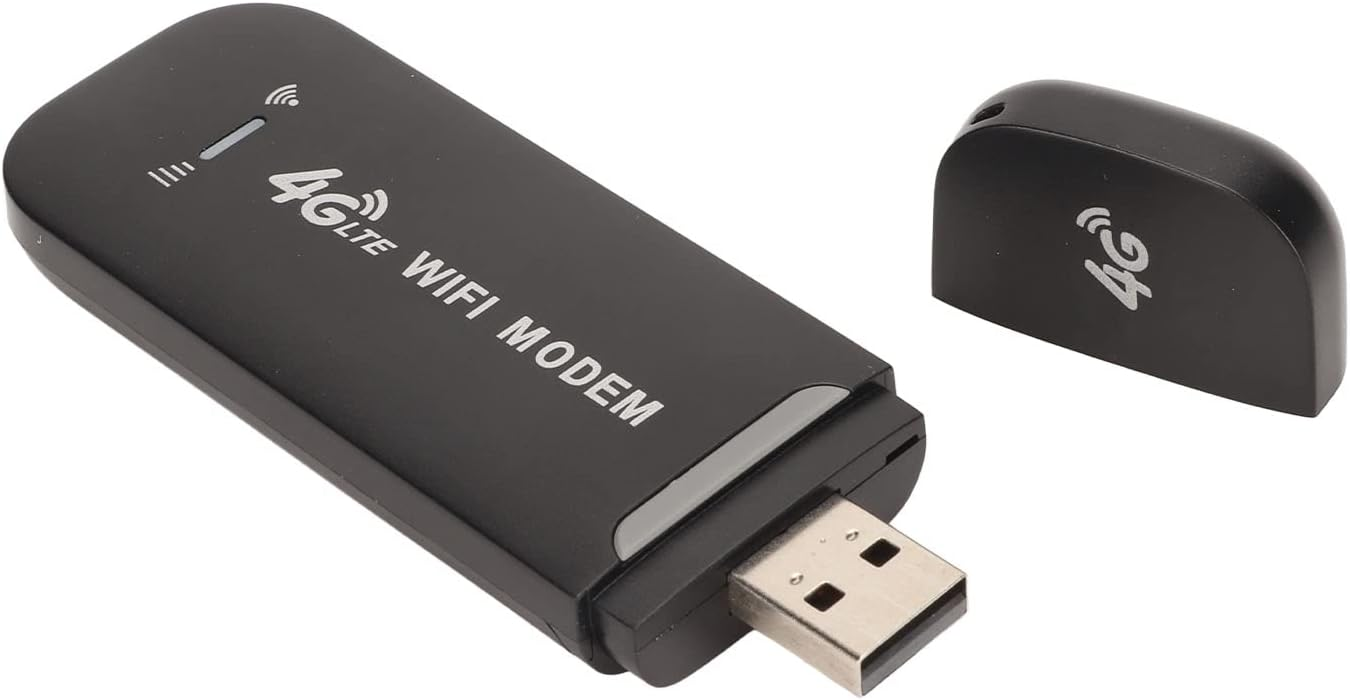
\includegraphics[width=0.5\textwidth]{img/herramientas/enrutador_wifi.png}
    \caption{Enrutador WiFi USB 4G LTE.} \label{Img:EnrutadorWifi}
\end{figure}

\subsection{Batería externa 20000 mAh}
Es un Power Bank~\cite{misc:Powerbank} portátil diseñado para cargar dispositivos móviles de forma rápida y eficiente. Con dos salidas USB-A y una entrada Type-C, proporciona flexibilidad para cargar múltiples dispositivos simultáneamente y recargarse fácilmente. Fabricada con aleación de aluminio, esta mini Powerbank, en elegante color gris, ofrece durabilidad y un diseño compacto que facilita su transporte. Con una capacidad de 20000mAh, es ideal para mantener tus dispositivos cargados mientras estás en movimiento, ya sea en viajes, actividades al aire libre o situaciones de emergencia.

\begin{table}[htbp]
\begin{center}
\caption{Características de la batería externa 20000 mAh.}
\begin{tabular}{|l|l|}
\hline
\rowcolor[HTML]{C0C0C0} 
\textbf{Característica} & \textbf{Descripción}\\ \hline
Tipo de conector entrada & usb tipo C (5V/2A)\\ \hline
Tipo de conector salida & usb tipo A2 (5V/2A)\\ \hline
Marca & YWTESCH \\ \hline
Color & Gris \\ \hline
Tensión & 5 voltios \\ \hline
Amperaje & 2 A \\ \hline
Capacidad máxima & 20000 mAh \\ \hline
Número de puertos & 2 \\ \hline
tamaño & 108$\times$69$\times$26 mm \\ \hline
\end{tabular}
\end{center}
\end{table}

\begin{figure}[h]
    \centering
    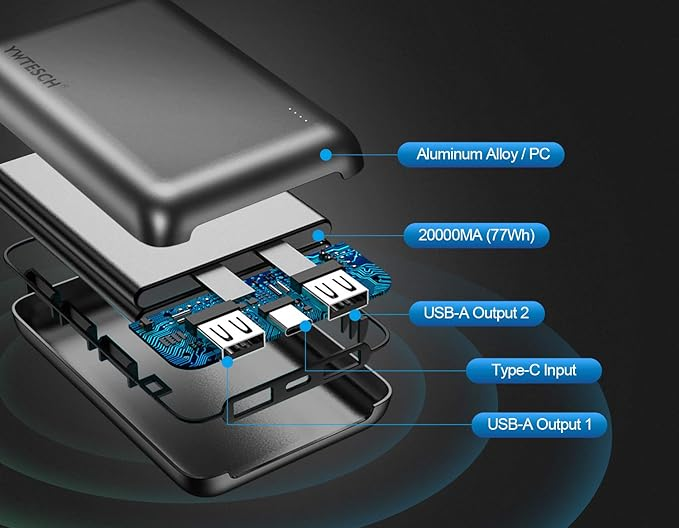
\includegraphics[width=0.6\textwidth]{img/herramientas/bateria_externa_descripcion.png}
    \caption{Batería externa 20000 mAh.} \label{Img:BateriaExterna}
\end{figure}

\subsection{Panel solar IP65 de 8W y 5V con cargador USB tipo C}
Este Panel Solar~\cite{misc:PanelSolar} es una solución eficiente para la carga de dispositivos móviles utilizando energía solar. Es una opción versátil para cargar dispositivos compatibles, como teléfonos, tabletas y otros dispositivos alimentados por USB. Compacto y fácil de transportar, es ideal para actividades al aire libre, viajes y situaciones donde la carga convencional no está disponible.

\begin{table}[htbp]
\begin{center}
\caption{Características del panel solar.}
\begin{tabular}{|l|l|} %|c|c|
\hline
\rowcolor[HTML]{C0C0C0} 
\textbf{Característica} & \textbf{Descripción}\\ \hline
USB & Tipo C con cable de 3 m \\ \hline
Capacidad & 8W y 5V \\ \hline
Material del panel & Silicio monocristalino \\ \hline
Vida útil & 20 años \\ \hline
Accesorios & Soporte ajustable 360$^\circ$ con tornillos y tojinos \\ \hline
Dimensiones & 23$\times$18.5$\times$1 cm\\ \hline
Tipo de protección & IP65 (resistente al polvo y agua)\\ \hline
\end{tabular}
\end{center}
\end{table}

\begin{figure}[h]
    \centering
    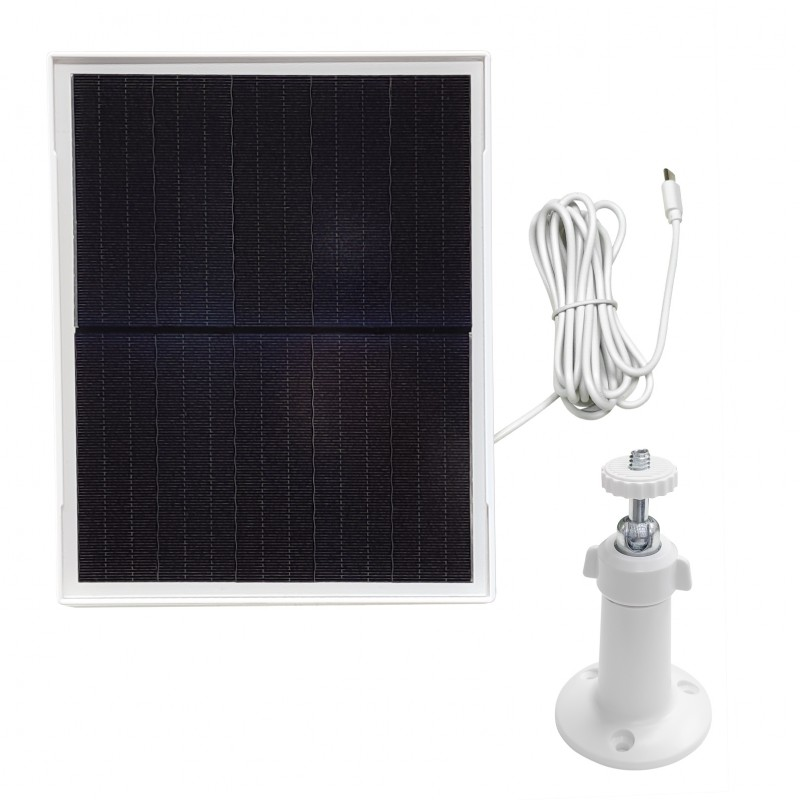
\includegraphics[width=0.7\textwidth]{img/herramientas/panel_solar.png}
    \caption{Panel solar y soporte ajustable.} \label{Img:PanelSolar}
\end{figure}

%Esta parte de la memoria tiene como objetivo presentar las técnicas metodológicas y las herramientas de desarrollo que se han utilizado para llevar a cabo el proyecto. Si se han estudiado diferentes alternativas de metodologías, herramientas, bibliotecas se puede hacer un resumen de los aspectos más destacados de cada alternativa, incluyendo comparativas entre las distintas opciones y una justificación de las elecciones realizadas. 
%No se pretende que este apartado se convierta en un capítulo de un libro dedicado a cada una de las alternativas, sino comentar los aspectos más destacados de cada opción, con un repaso somero a los fundamentos esenciales y referencias bibliográficas para que el lector pueda ampliar su conocimiento sobre el tema.

\capitulo{5}{Aspectos relevantes del desarrollo del proyecto}

En esta sección, se destacarán los elementos más significativos del desarrollo, proporcionando una perspectiva detallada de las decisiones adoptadas para alcanzar los objetivos del proyecto. Se resumirá la experiencia práctica, detallando cómo se abordaron los desafíos específicos, y se evaluará la importancia de estas soluciones en el contexto general del alcance del proyecto.

\section{Motivación del proyecto}

La motivación subyacente a este proyecto surge de la creciente importancia y demanda en el ámbito de la monitorización de invernaderos, especialmente en el contexto del cultivo de cannabis medicinal. La necesidad de implementar soluciones tecnológicas eficientes para garantizar condiciones óptimas de cultivo y maximizar la producción ha impulsado la elección de este tema.

El objetivo principal radica en diseñar un sistema económico y eficaz que permita a los cultivadores de cannabis medicinal supervisar las condiciones ambientales de sus invernaderos de manera remota. Este proyecto busca proporcionar una herramienta valiosa para mejorar la eficiencia, la calidad y la consistencia en la producción de cannabis medicinal, al tiempo que se abordan los desafíos específicos asociados con la monitorización de variables críticas como temperatura, humedad y luz.

\section{Formación necesaria}

El proyecto ha requerido una formación interdisciplinaria que abarca diversas áreas. En primer lugar, la comprensión profunda de los principios de la programación y el desarrollo de software ha sido esencial. La elección de la Raspberry Pi Pico W como plataforma y la programación en MicroPython para controlar los dispositivos hardware involucra un conocimiento sólido en programación embebida y desarrollo en entornos limitados.

Además, la utilización de sensores especializados, como el DHT22~\cite{manual:DHT22}, el BH1750~\cite{manual:BH1750} y el sensor de humedad del suelo~\cite{wiki:SensorHumedadSuelo}, ha demandado una comprensión detallada de los principios de operación de estos dispositivos y cómo integrar sus lecturas en el sistema general. Esto implica una formación técnica en electrónica y sensores.

La implementación de conceptos relacionados con el Internet de las cosas (IoT) y la comunicación inalámbrica mediante la Raspberry Pi Pico W~\cite{misc:RPiPicoW} también ha requerido conocimientos específicos en redes y protocolos de comunicación.

La integración de MQTT~\cite{manual:MQTT} en el código MicroPython para la Raspberry Pi Pico W ha requerido conocimientos específicos sobre este protocolo de mensajería ligero diseñado para la eficiente comunicación entre dispositivos en redes IoT.

En resumen, la formación necesaria abarca habilidades en programación embebida, electrónica, redes, IoT y desarrollo de software. La combinación de estas competencias ha sido esencial para la ejecución exitosa del proyecto, demostrando la importancia de una formación integral y multidisciplinaria en el ámbito de la ingeniería y la tecnología.
\pagebreak

\section{Metodología}
Se ha optado por la metodología del \textbf{Modelo de Prototipos}~\cite{misc:Metodologia_ModeloDePrototipos} debido a su capacidad para proporcionar retroalimentación temprana, clarificar requisitos, adaptarse a cambios, validar prácticamente funcionalidades, reducir riesgos, comprender la interfaz de usuario y facilitar la mejora continua. Este enfoque iterativo permite identificar y corregir problemas desde las primeras etapas, garantizando la eficiencia y el éxito en el desarrollo del sistema IoT de monitorización de invernaderos de cannabis medicinal.

\subsection{Identificación de Requisitos Iniciales:}
\textbf{Hardware:}
\begin{itemize}
	\item Raspberry Pi Pico W~\cite{misc:RPiPicoW} como la plataforma central.
	\item Sensores DHT22~\cite{manual:DHT22} para medir temperatura y humedad ambiente.
	\item Sensor BH1750~\cite{manual:BH1750} para evaluar la intensidad de luz.
	\item Sensor de humedad de suelo~\cite{wiki:SensorHumedadSuelo} para monitorizar las condiciones del suelo.
	\item Pantalla OLED~\cite{manual:Oled} para visualización de datos.
	\item LEDs RGB~\cite{manual:LedRGB} para indicar condiciones críticas.
\end{itemize}

\textbf{Software:}
\begin{itemize}
	\item Desarrollo de un sistema en MicroPython para la Raspberry Pi Pico W~\ref{proyecto:Hardware}.
	\item Implementación de un servidor LAMP para almacenar y gestionar datos.
	\item Integración de la API de Telegram~\cite{misc:Telegram_api} para recibir alertas.
	\item Aplicación de escritorio para Windows~\ref{proyecto:InverIoT}, desarrollada en Visual Studio 2022 en lenguaje C\#. Incluye su instalador.
	\item Dashboard web~\ref{proyecto:Dashboard}, realizado con Node.js, accesible desde internet.
\end{itemize}

\textbf{Funcionalidades clave:}
\begin{itemize}
	\item Captura de datos ambientales como temperatura, humedad, luz y humedad del suelo.
	\item Representación gráfica de los datos en una pantalla OLED.
	\item Envío de alertas a través de Telegram en caso de valores fuera de los umbrales ideales.
	\item Interacción bidireccional para activar mecanismos de respuesta a condiciones ambientales adversas.
\end{itemize}

\subsection{Desarrollo del Primer Prototipo:}
En esta etapa, se enfocó en la integración de los componentes hardware definidos, como la Raspberry Pi Pico W~\cite{misc:RPiPicoW} y los sensores de humedad, temperatura~\cite{manual:DHT22}, luminosidad~\cite{manual:BH1750} y humedad del suelo~\cite{wiki:SensorHumedadSuelo}. Se estableció la conexión con el servidor LAMP utilizando MQTT~\cite{manual:MQTT} para la transmisión de datos en tiempo real.

Durante la fase de desarrollo, se configuraron y probaron los mecanismos de alerta a través del bot de Telegram y la activación de los LEDs RGB para indicar condiciones críticas. También se diseñó e implementó la lógica de umbrales para verificar si los valores ambientales están dentro de los límites ideales.

\subsection{Evaluación del Primer Prototipo:}
El objetivo principal fue validar la efectividad de las funcionalidades implementadas y su capacidad para cumplir con los requisitos planteados en la fase inicial del proyecto.
\begin{itemize}
	\item \textbf{Pruebas de Mecanismos de Alerta y Retroalimentación Visual:}
Se realizaron pruebas del sistema de alertas a través del bot de Telegram. Se verificó la capacidad del sistema para enviar notificaciones en tiempo real sobre condiciones ambientales críticas, como temperaturas extremas o niveles de humedad fuera de los umbrales establecidos.

Además, se evaluó la respuesta de los LEDs RGB conectados, los cuales indican visualmente las condiciones del entorno. Cada color del LED se asoció con un estado específico, permitiendo una retroalimentación instantánea sobre el estado actual del invernadero.
\item \textbf{Verificación de la Lógica de Umbrales:}
La lógica de umbrales, diseñada para verificar si los valores ambientales se mantienen dentro de los límites ideales, está en fase de pruebas en un entorno no controlado. En este contexto, se observa que los valores experimentan salidas fuera de los umbrales establecidos. Sin embargo, se ha verificado con éxito que la lógica implementada para activar las alertas funciona de manera efectiva cuando los valores se desvían de los límites ideales predefinidos.
\end{itemize}
\subsection{Retroalimentación y Mejoras:}
Tras la evaluación del primer prototipo, se recopiló retroalimentación valiosa para orientar mejoras futuras. Se identificaron áreas de oportunidad, como la necesidad de ajustar los umbrales para adaptarse a condiciones específicas del entorno y mejorar la precisión de las alertas. La retroalimentación del usuario sobre la interfaz y la usabilidad también se tuvo en cuenta para realizar ajustes en el diseño del dashboard web y la aplicación de escritorio. Estas observaciones se utilizarán como guía para la siguiente iteración del prototipo, buscando una mayor eficiencia y adecuación a los requisitos específicos del sistema.

\subsection{Desarrollo de Subsiguientes Prototipos:}
Con base en la retroalimentación obtenida del primer prototipo, se inició el desarrollo de subsiguientes prototipos con el objetivo de implementar mejoras significativas. Se priorizó la optimización de los umbrales de alerta, considerando las condiciones específicas del entorno de monitoreo. También se abordaron ajustes en la interfaz del dashboard web y la aplicación de escritorio, respondiendo a las sugerencias de los usuarios para mejorar la usabilidad y la experiencia general. Cada nuevo prototipo se sometió a pruebas exhaustivas para validar las mejoras implementadas y garantizar un funcionamiento más eficiente del sistema en su conjunto. Este proceso iterativo permitió refinamientos continuos, enfocados en lograr un sistema de monitoreo más preciso y adaptado a las necesidades específicas del usuario.

\subsection{Validación Continua:}
Se llevaron a cabo pruebas exhaustivas para verificar el funcionamiento del sistema, evaluando diversos escenarios y condiciones ambientales para confirmar la precisión de los sensores y la respuesta del sistema. Se realizaron pruebas de estrés para evaluar la capacidad de respuesta en situaciones extremas.

Durante un período prolongado, se recopilaron datos para analizar el rendimiento a lo largo del tiempo, comparándolos con los umbrales ideales establecidos. Algunos valores se salieron del rango ideal debido a las pruebas en un entorno no controlado, pero se verificó que el sistema funcionó correctamente y generó alertas de manera adecuada al encontrarse en un ambiente controlado.

La retroalimentación continua de las pruebas y la validación de los resultados se utilizaron para ajustar el sistema, mejorando su robustez y confiabilidad. Este ciclo de validación y ajuste continuo contribuyó a optimizar el sistema para lograr un monitoreo preciso y eficiente de las condiciones del invernadero.

\subsection{Integración de Componentes:}
Durante esta etapa, se procedió a la integración de los diferentes componentes del sistema. Se conectaron y configuraron la Raspberry Pi Pico W~\cite{misc:RPiPicoW} como plataforma central, junto con los sensores DHT22, BH1750~\cite{manual:BH1750} y el sensor de humedad del suelo~\cite{wiki:SensorHumedadSuelo}. Se aseguró la comunicación efectiva entre estos elementos, permitiendo la captura precisa de datos ambientales.

El desarrollo de un sistema en MicroPython~\cite{wiki:micropython} para la Raspberry Pi Pico W se integró con éxito con el servidor LAMP, facilitando la gestión y almacenamiento de datos. La implementación de la API de Telegram~\cite{misc:Telegram_api} se conectó con el sistema para recibir alertas en tiempo real.

La aplicación de escritorio para Windows~\ref{proyecto:InverIoT}, desarrollada en Visual Studio 2022 con lenguaje C\#~\cite{manual:CSharp}, se integró sin problemas, permitiendo la visualización de datos en tiempo real y la interacción bidireccional con el sistema.

El dashboard web~\ref{proyecto:Dashboard}, creado con Node.js, se integró para ofrecer una interfaz accesible a través de internet, proporcionando una visualización completa y en tiempo real de los datos capturados. Esta etapa de integración aseguró la cohesión y el funcionamiento conjunto de todos los componentes del sistema IoT para el monitoreo de invernaderos.

\subsection{Ajustes Finales:}
Estos ajustes se centraron en mejorar la precisión de los sensores, la eficacia de las alertas y la respuesta de los mecanismos de control. Se llevaron a cabo modificaciones en el código del sistema para perfeccionar la lógica de umbrales y asegurar que los valores se mantuvieran dentro de los límites ideales.

Además, se realizaron ajustes en la configuración de la pantalla OLED y los LEDs RGB para una visualización más clara y distintiva de las condiciones del invernadero. La interfaz de usuario se mejoró para facilitar la comprensión de los datos mostrados en tiempo real. También se realizaron pruebas adicionales para verificar la estabilidad del sistema en condiciones diversas.

Este proceso de ajustes finales contribuyó a la optimización global del sistema, asegurando un monitoreo preciso y una respuesta efectiva a las variaciones ambientales en el invernadero. La retroalimentación continua y la iteración fueron fundamentales en esta fase para lograr un prototipo final robusto y funcional.

\subsection{Documentación:}
Se elaboró una documentación completa que abarca aspectos técnicos, funcionales y de implementación del sistema desarrollado. La documentación detallada incluye manuales de usuario para las distintas interfaces, descripciones técnicas de hardware y software, así como instrucciones para la instalación y configuración del sistema.

Además, se generaron documentos específicos para el mantenimiento del sistema, facilitando futuras actualizaciones y mejoras.

Esta documentación sirve como recurso integral para cualquier persona que interactúe con el sistema, desde usuarios finales hasta desarrolladores o técnicos de mantenimiento. Su elaboración garantiza la comprensión y el uso efectivo del sistema, contribuyendo a su sostenibilidad a lo largo del tiempo.

\subsection{Implementación Final:}
La implementación final del sistema se llevó a cabo tras la validación y ajustes continuos a lo largo de las fases de desarrollo y prototipado. En esta etapa, se consolidaron todas las funcionalidades y características planificadas, integrando los componentes hardware y software de manera coherente.

Se realizó una verificación exhaustiva de la interacción entre los sensores, la Raspberry Pi Pico W, la pantalla OLED, y los LEDs RGB. Se mejoró la respuesta del sistema ante condiciones ambientales diversas y se afinaron los algoritmos de control para garantizar un monitoreo preciso y eficiente del invernadero.

Además, se implementaron las últimas medidas de seguridad y se realizaron pruebas exhaustivas para garantizar la estabilidad del sistema en distintos escenarios. Se documentaron detalladamente los pasos necesarios para replicar la implementación final, asegurando una fácil reproducción y mantenimiento.

La implementación final refleja la evolución del sistema desde su concepción hasta la etapa de producción, consolidando todas las lecciones aprendidas durante el desarrollo y prototipado.

\section{Desarrollo del proyecto}

El propósito inicial radicaba en la recopilación de datos ambientales, tales como humedad, temperatura, intensidad de luz y humedad del suelo, con el fin de almacenarlos y presentarlos de manera gráfica.

Con este propósito, se optó por la Raspberry Pi Pico W debido a su eficiencia energética y coste accesible. Se conectaron al sistema un sensor de humedad y temperatura DHT22~\cite{manual:DHT22}, un sensor de intensidad de luz BH1750~\cite{manual:BH1750}, y un sensor de humedad de suelo~\cite{wiki:SensorHumedadSuelo}. Además, se incorporaron LEDs RGB~\cite{manual:LedRGB} para señalizar alertas. A esta parte del proyecto se ha llamado \textbf{Hardware}~\ref{proyecto:Hardware}.

\begin{figure}[h]
	\centering
	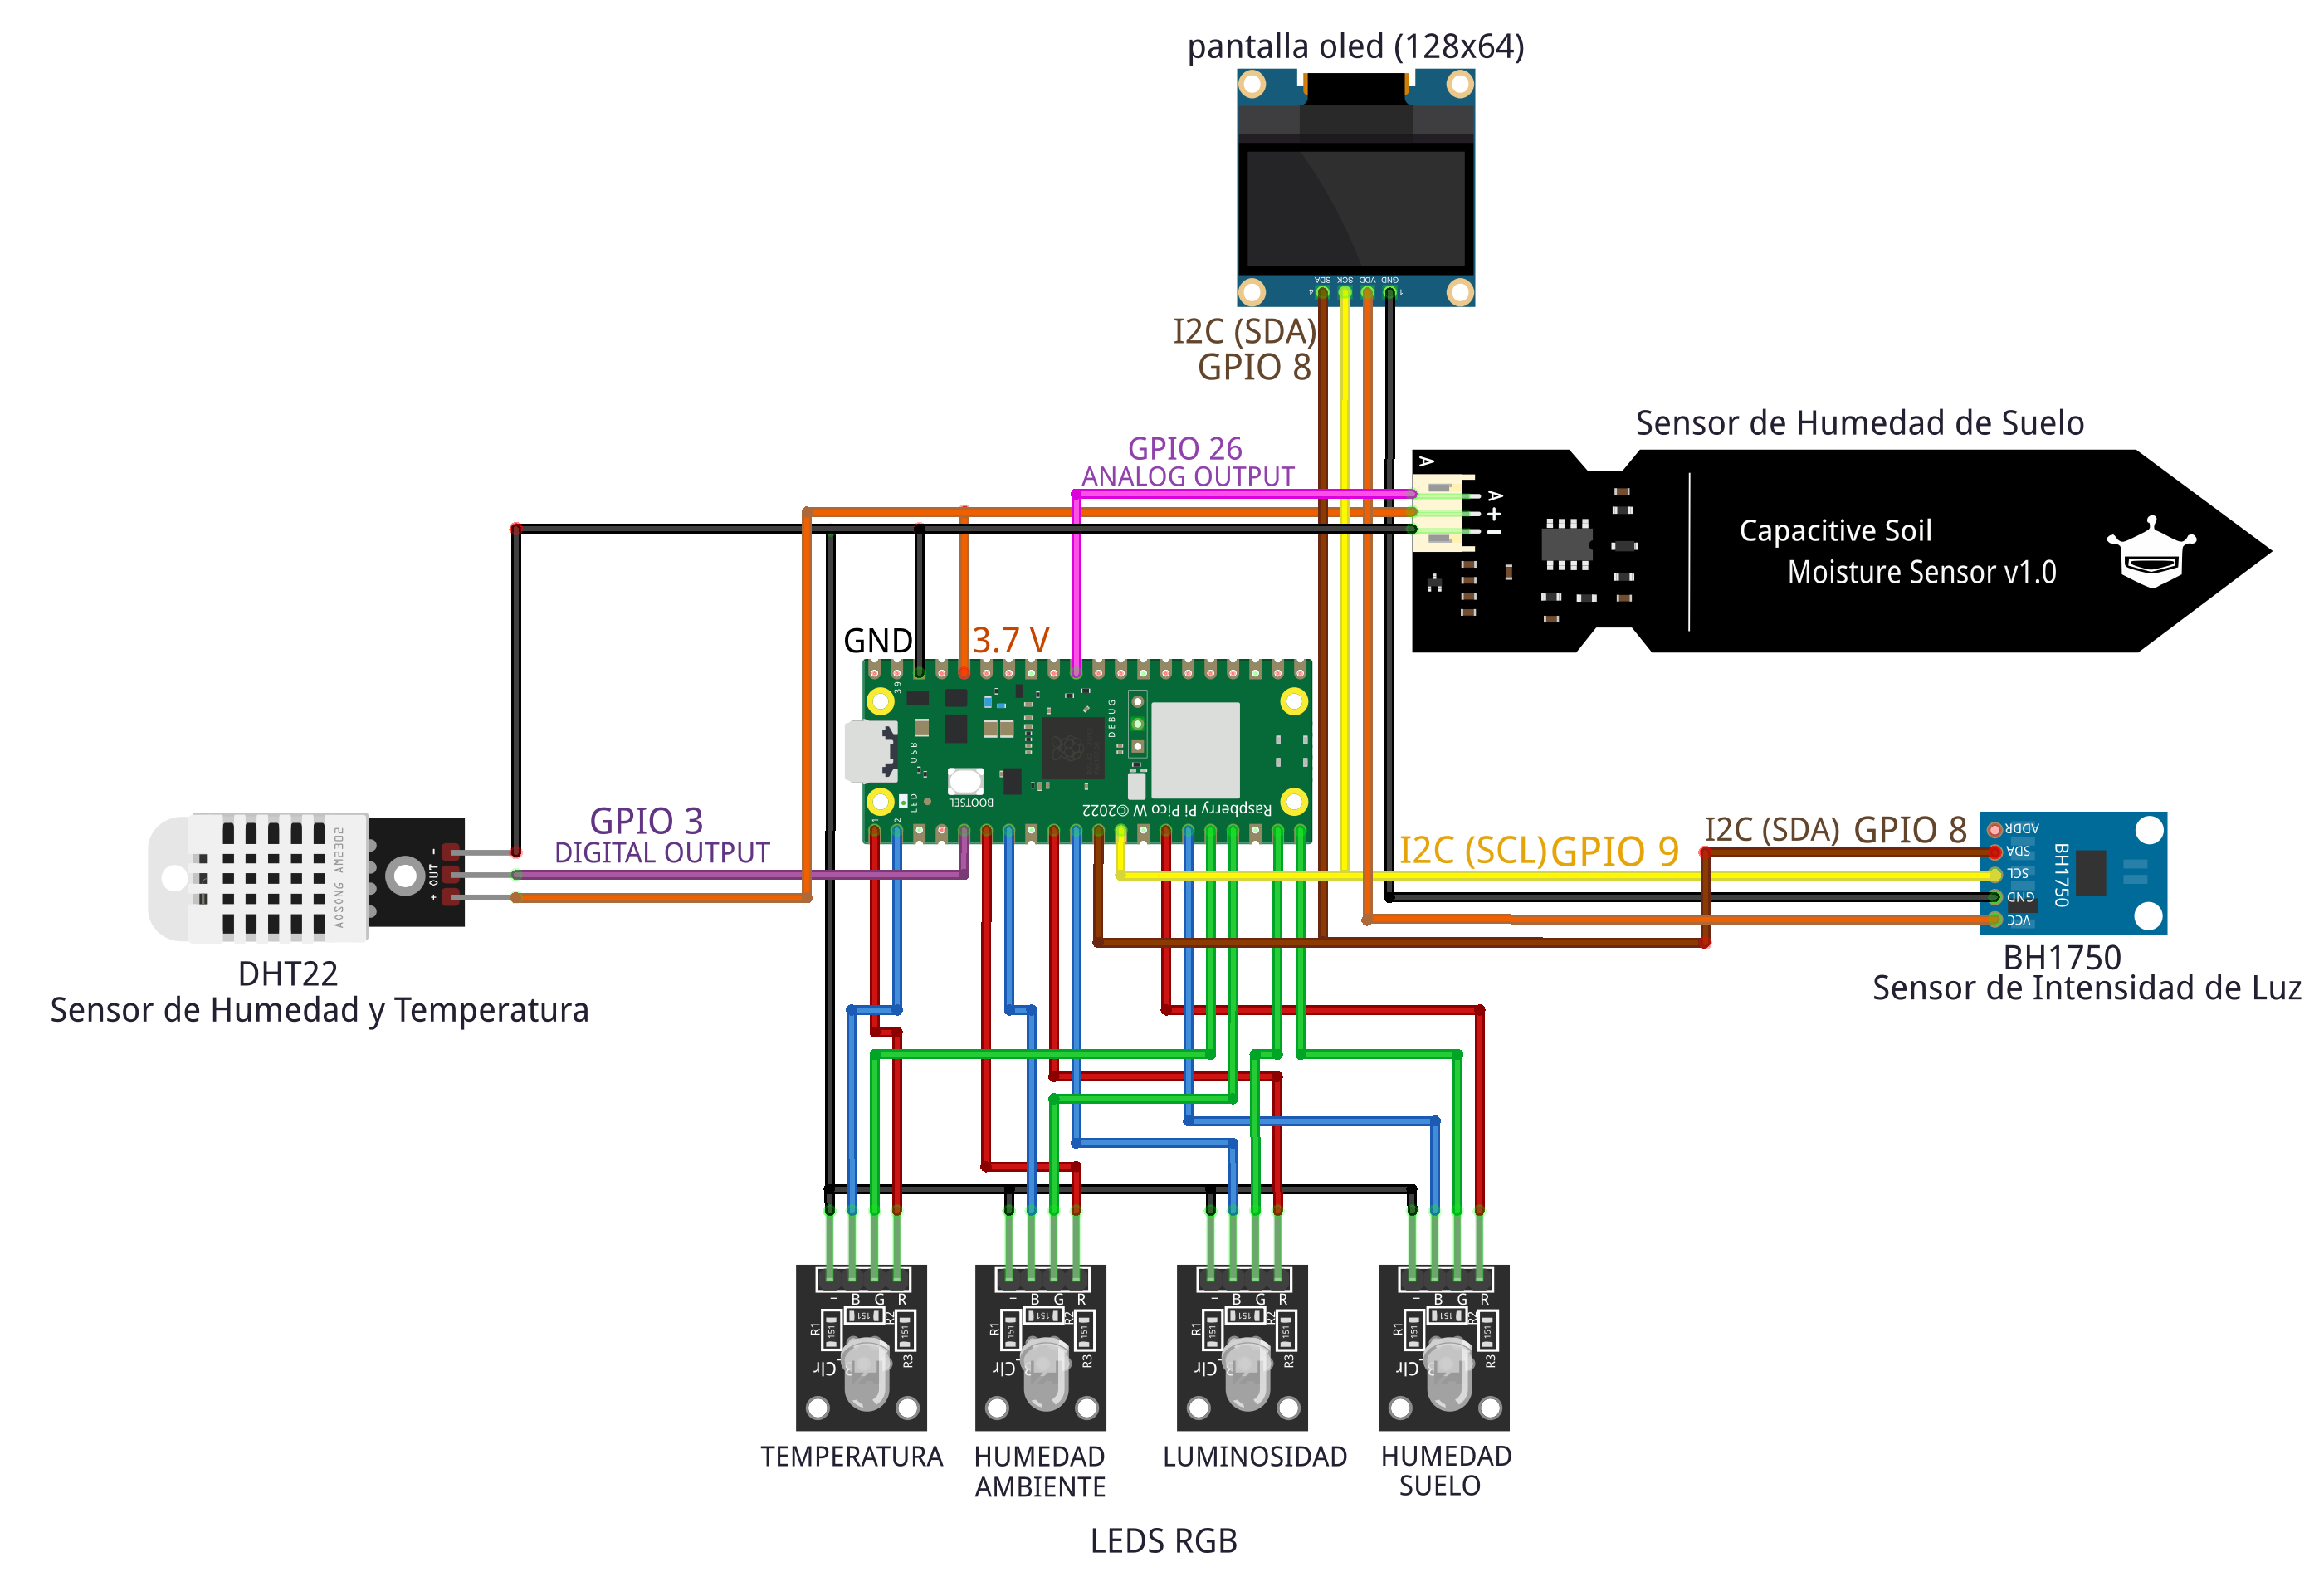
\includegraphics[width=0.8\textwidth]{img/diagramas/conexiones_simple.png}
	\caption{Raspberry Pi Pico W conectada a sensores y una pantalla oled.} \label{Img:conexion_simple}
\end{figure}

\begin{figure}[h]
	\centering
	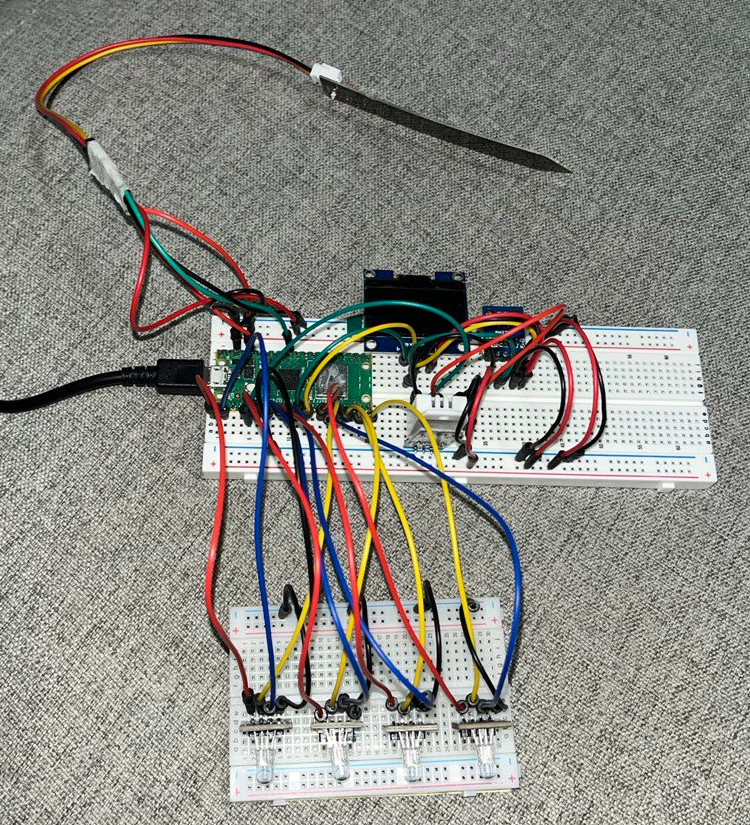
\includegraphics[width=0.4\textwidth]{img/fotos/conexiones_real.png}
	\caption{Raspberry Pi Pico W y sensores conectados mediante un protoboard.} \label{Img:conexion_simple}
\end{figure}

Una vez definida la idea del TFG y los componentes hardware, surgía la interrogante: "¿Dónde enviar los datos? ¿Cómo gestionarlos?". La primera medida fue mostrar los datos en una pantalla OLED~\cite{manual:Oled} conectada a la protoboard.

\begin{figure}[h]
	\centering
	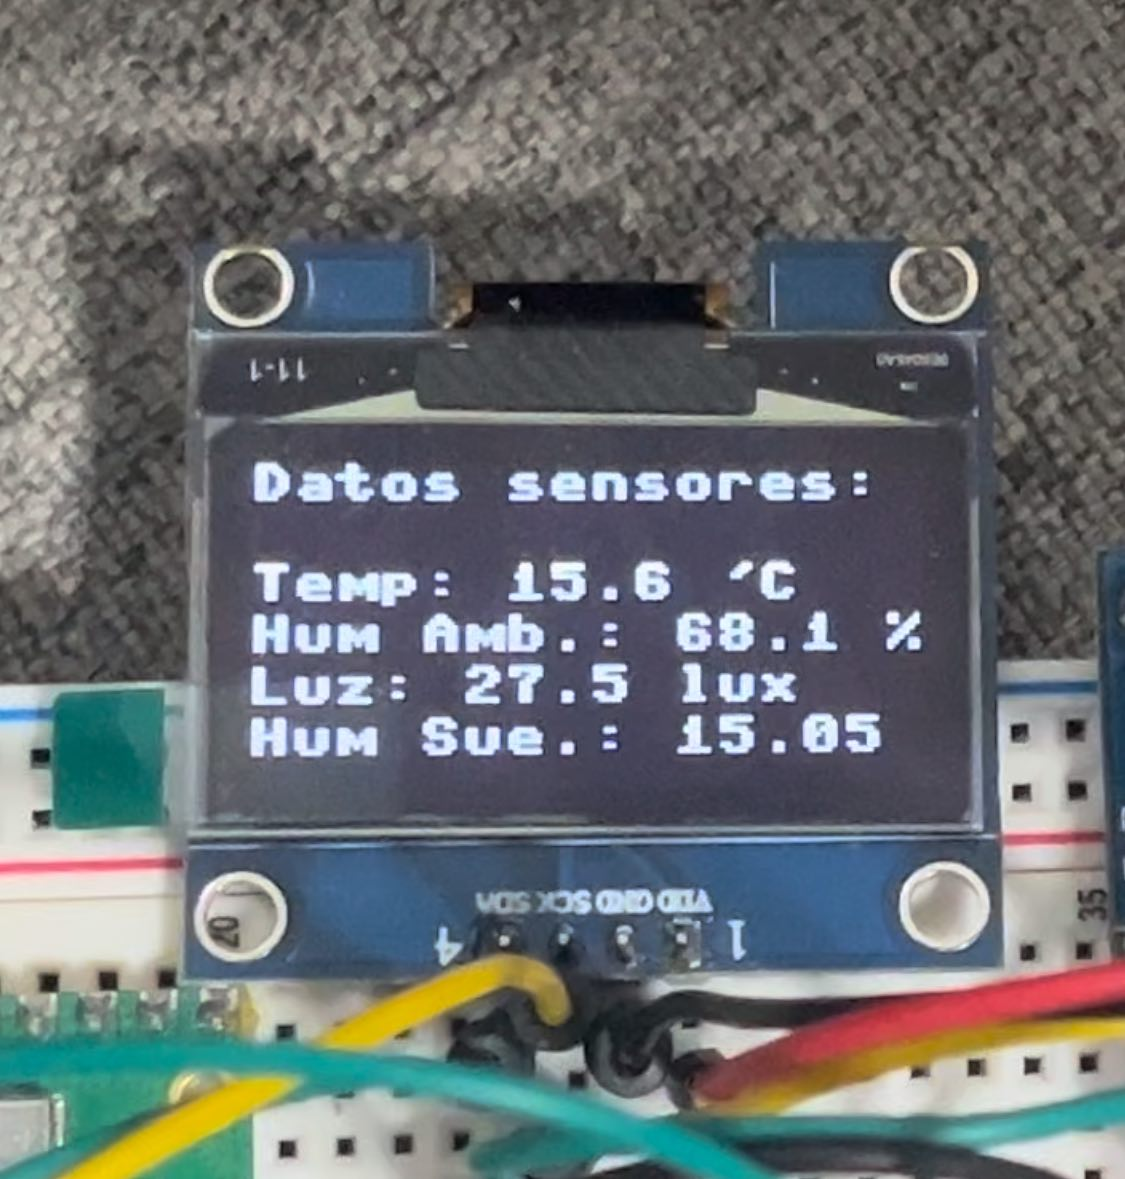
\includegraphics[width=0.4\textwidth]{img/fotos/oled1.png}
	\caption{Pantalla oled conectada a la Raspberry Pi Pico W.} \label{Img:oled_conexion}
\end{figure}

Sin embargo, al estar fuera de la red, surgieron nuevas incógnitas, ya que inicialmente se trató de un sistema unidireccional en el cual el sensor recolecta los datos y los muestra en la pantalla OLED.

Más tarde, se implementó la funcionalidad de enviar alertas a través de Telegram en caso de que los valores recopilados excedieran los umbrales ideales.

\begin{figure}[h]
	\centering
	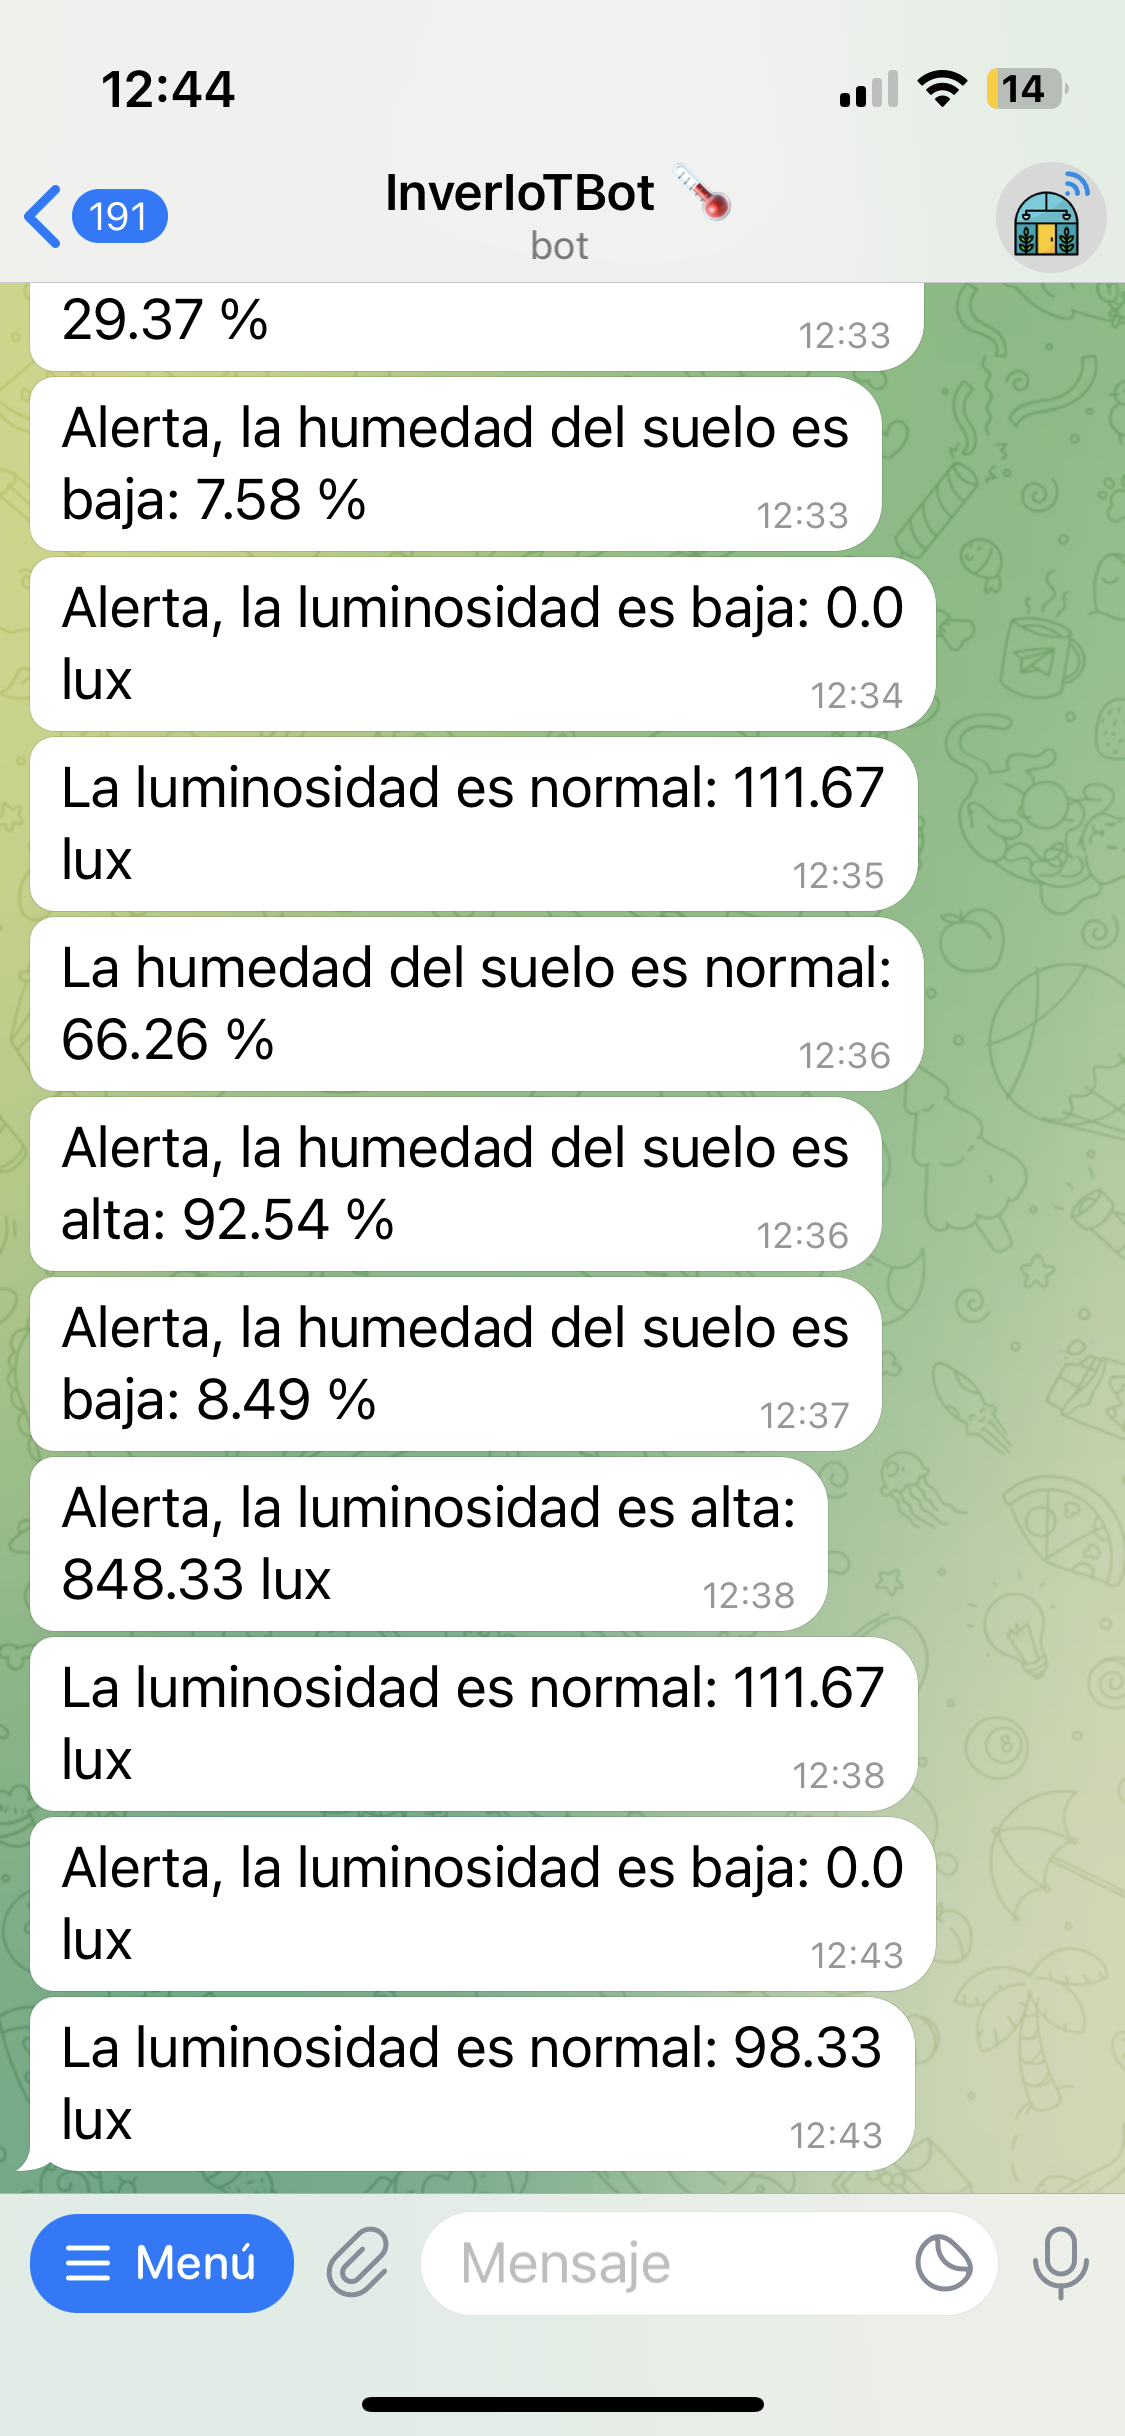
\includegraphics[width=0.27\textwidth]{img/desarrollo/BotTelegram_alertas.png}
	\caption{Alertas del bot de Telegram.} \label{Img:BotTelegram_alertas}
\end{figure}

Posteriormente, opté por establecer un servidor LAMP para facilitar el envío y manejo de datos. La implementación de este servidor se llevó a cabo en el sistema operativo Ubuntu~\cite{misc:Ubuntu}, el cual fue virtualizado utilizando Hyper-V~\cite{manual:Hyper_V}.
En esta instancia, se emplea un servidor físico HP ProLiant~\cite{misc:HP_ProLiant} para la virtualización de los servicios Apache~\cite{misc:Apache}, MySQL~\cite{misc:Mysql}, PHP~\cite{misc:PHP} y SSH~\cite{misc:SSH}.

\begin{table}[htbp]
\begin{center}
\caption{Características del servidor HP ProLiant.}
\begin{tabular}{|l|l|}
\hline
\rowcolor[HTML]{C0C0C0} 
\textbf{Característica} & \textbf{Descripción}\\ \hline
Sistema operativo & Windows Server 2019 Standard\\ \hline
Fabricante & Hewlett Packard Enterprise \\ \hline
Modelo & Hewlett Packard Enterprise x64 Class PC\\ \hline
Procesador & Intel(R) Xeon(R) Silver 4210R CPU @ 2.4GHz 2.39GHz\\ \hline
Memoria instalada (RAM) & 128 GB (128 GB utilizable) \\ \hline
Tipo de sistema & Sistema operativo de 64 bits, procesador x64 \\ \hline
\end{tabular}
\end{center}
\end{table}

\begin{figure}[h]
	\centering
	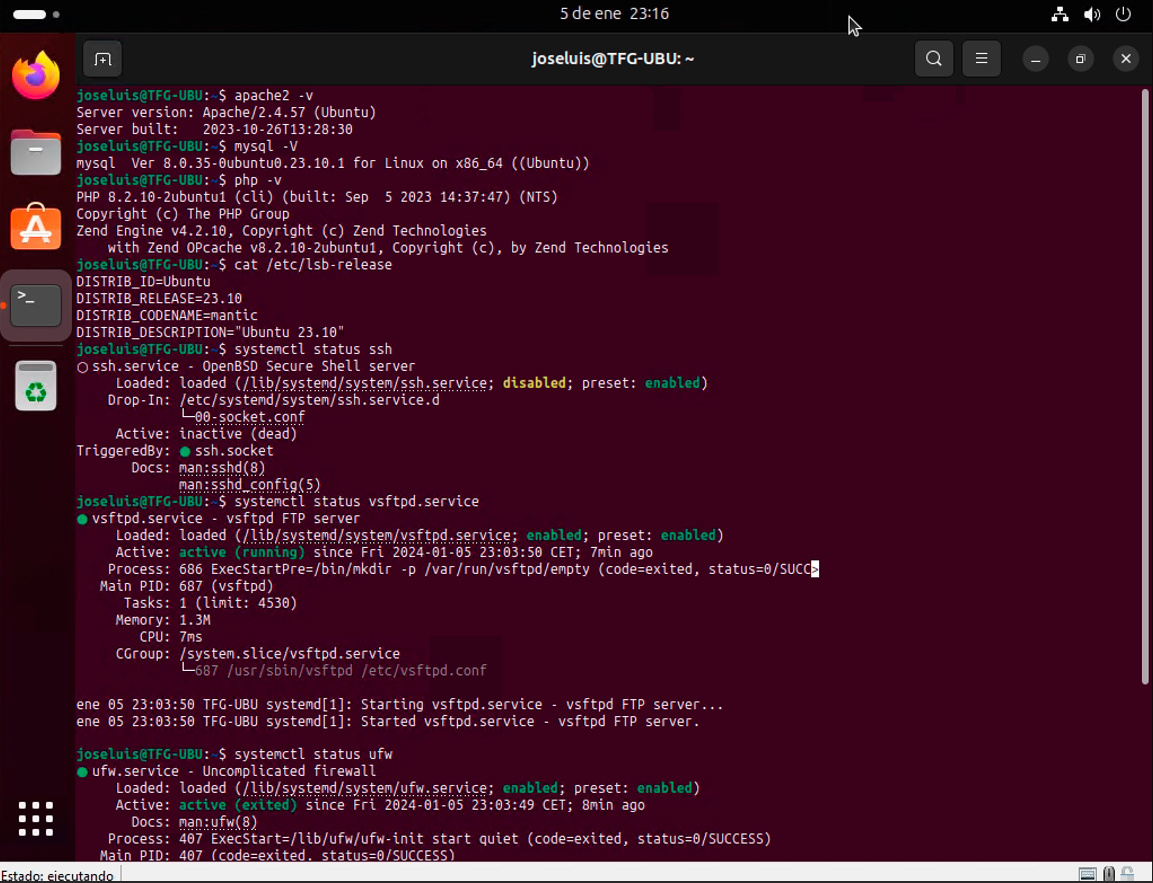
\includegraphics[width=1\textwidth]{img/desarrollo/LAMP_servicios.png}
	\caption{Servicios instalados y operativos en el servidor LAMP.} \label{Img:LAMP_servicios}
\end{figure}

Basándome en esta información y en mi experiencia previa trabajando con \textbf{Smart Cities}, tomo la decisión de enviar la información recopilada por los sensores al servidor mediante MQTT~\cite{manual:MQTT}. 

\begin{figure}[h]
	\centering
	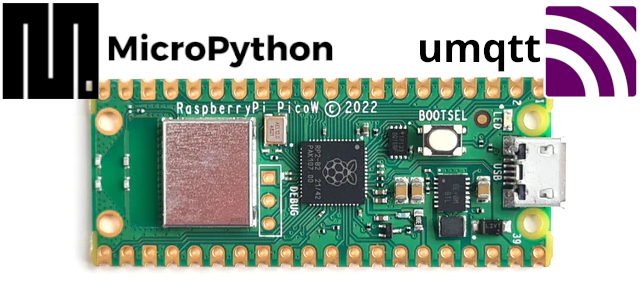
\includegraphics[width=0.7\textwidth]{img/herramientas/rpipicow_umqtt.png}
	\caption{Se ha implementado la libreria umqtt en la Raspberry Pi Pico W.} \label{Img:rpipicow_umqtt}
\end{figure}

MQTT permite la visualización en tiempo real de los datos en una página web alojada en el servidor LAMP cada vez que la placa junto con el sensor envíe datos. Además, posibilita el almacenamiento de los datos en la base de datos MySQL~\cite{misc:Mysql}, permitiéndome mantener un historial y realizar consultas. A esta parte del proyecto se ha llamado \textbf{NodeMqtt}~\ref{proyecto:NodeMqtt}.

\begin{figure}[h]
	\centering
	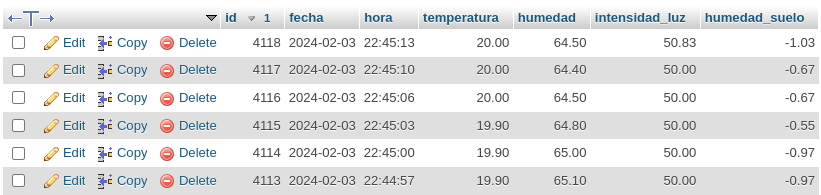
\includegraphics[width=1\textwidth]{img/desarrollo/mysql_data.png}
	\caption{Data almacenada en la base de datos.}
\end{figure}

Listo, he leído e incluso almacenado los datos que se envían. Además, con la implementación de un bot de Telegram~\cite{misc:Telegram}, ahora puedo consultar en tiempo real la información proveniente de los sensores.

\begin{figure}[h]
	\centering
	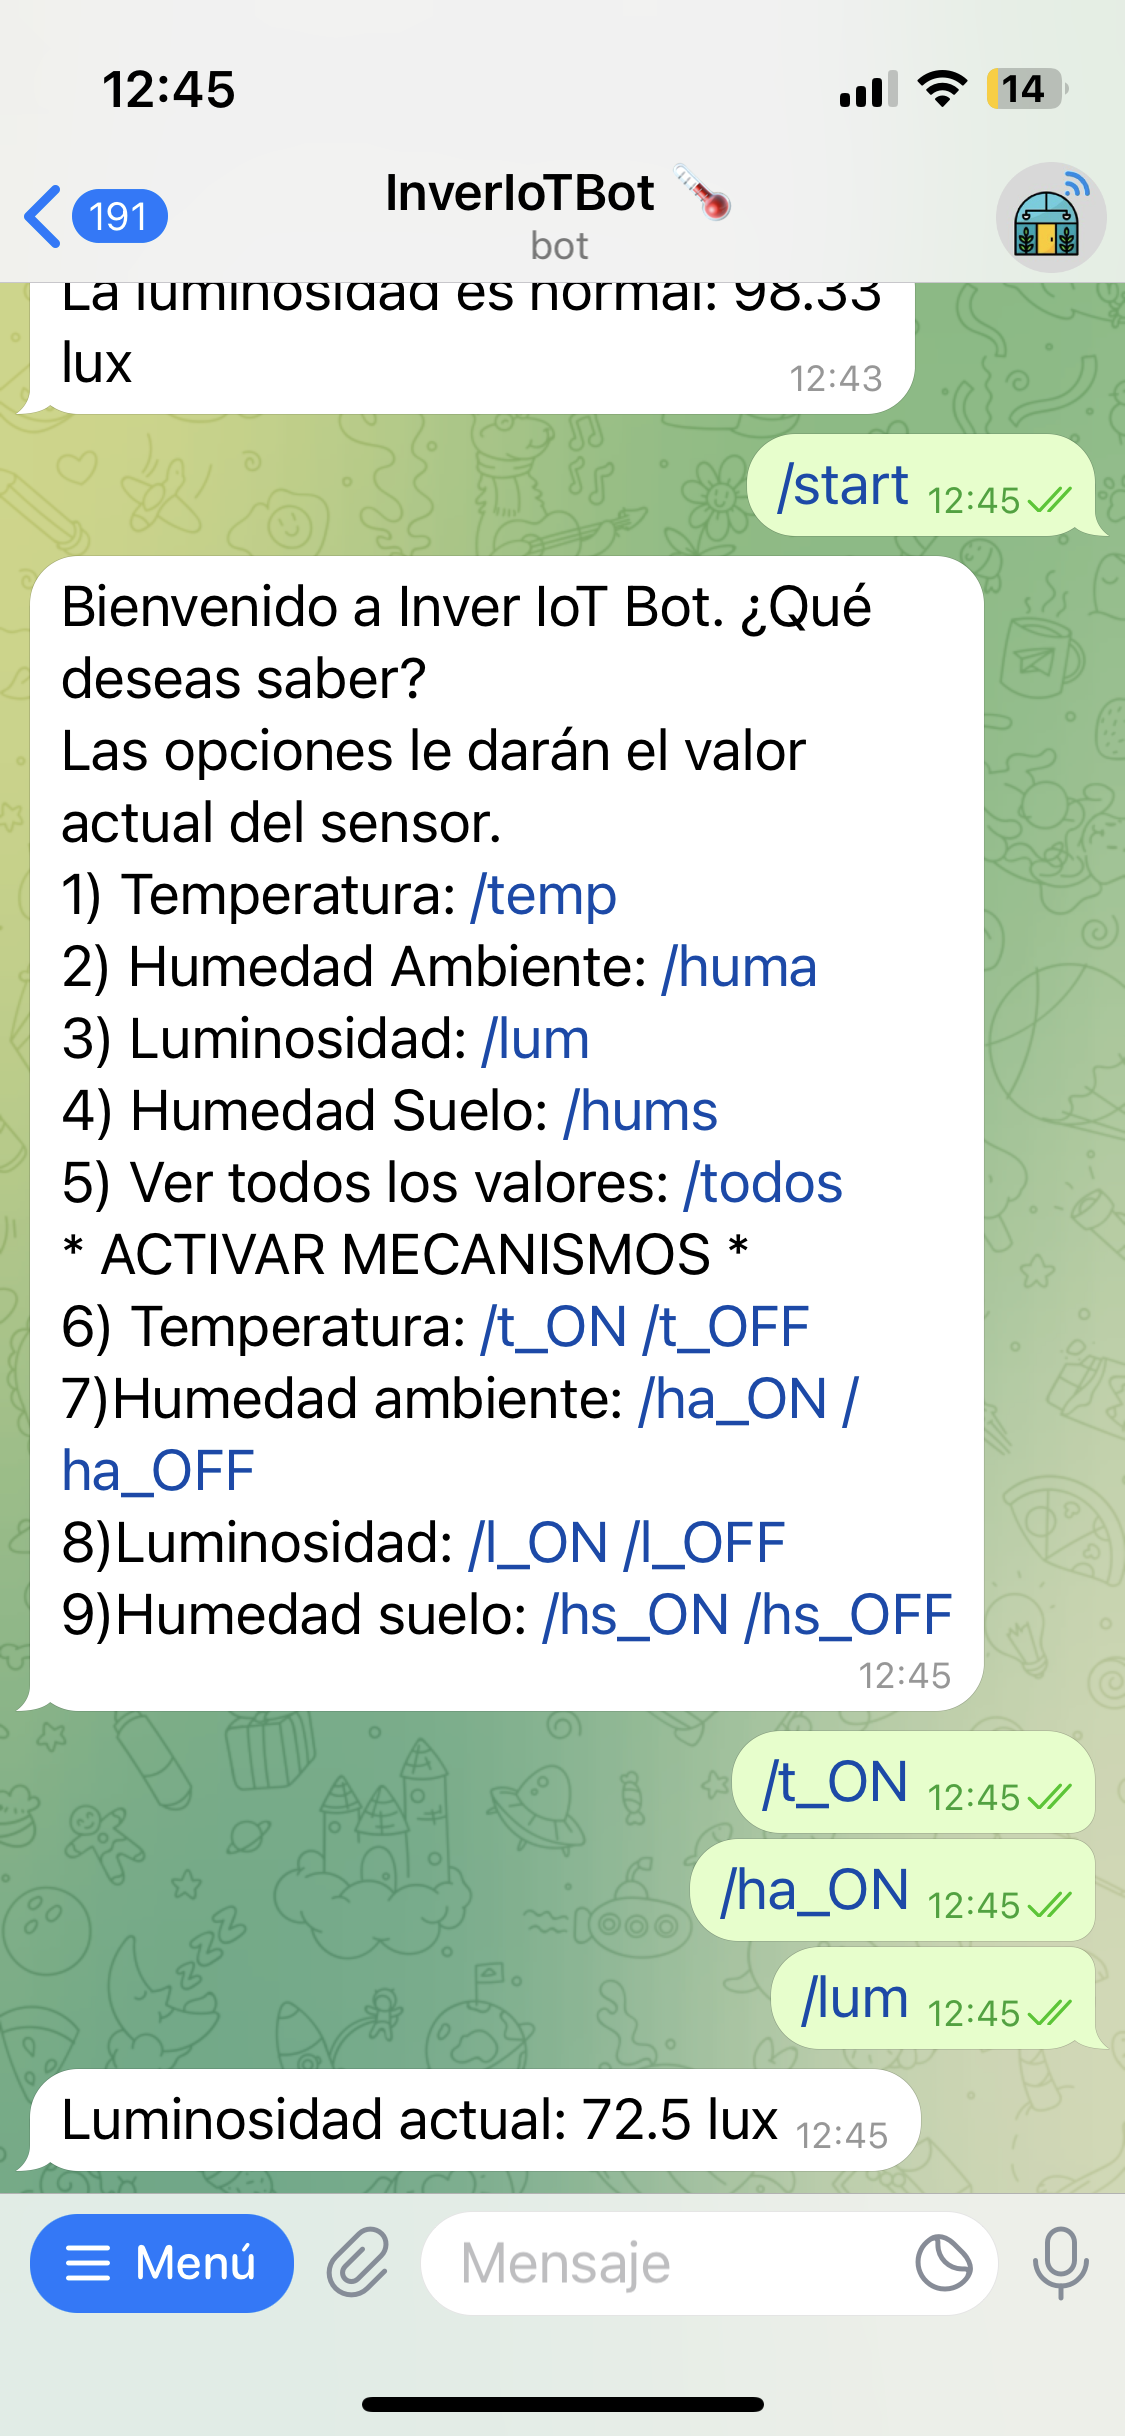
\includegraphics[width=0.32\textwidth]{img/desarrollo/BotTelegram_comandos.png}
	\caption{Consulta a la base de datos mediante comandos usando Telegram.}
\end{figure}

También optamos por desarrollar una aplicación de escritorio para Windows en C\#~\cite{manual:CSharp} al que se ha llamado \textbf{InverIoT}~\ref{proyecto:InverIoT}, que permite la visualización en tiempo real de los datos. ¡Problema resuelto! Ahora, puedo recibir y monitorear la temperatura, luminosidad y otros valores del invernadero.

\begin{figure}[h]
	\centering
	\includegraphics[width=0.61\textwidth]{img/fotos/InverIoT_PasandoUmbralLuz.png}
	\caption{El led rojo y el color naranja en la aplicación InverIoT indican que se ha sobrepasado el umbral de luz.}
\end{figure}

Sin embargo, al caer la noche, la luminosidad y la temperatura disminuyen, planteando un nuevo desafío. En este caso, necesitaría establecer una comunicación bidireccional con la placa Raspberry Pi Pico W para, por ejemplo, encender los focos y activar los calentadores.

Este cambio a una comunicación bidireccional se logró suscribiendo la Raspberry Pi Pico W a un topic MQTT. Ahora, puedo enviar órdenes para procesarlas según sea necesario. 

\begin{figure}[h]
	\centering
	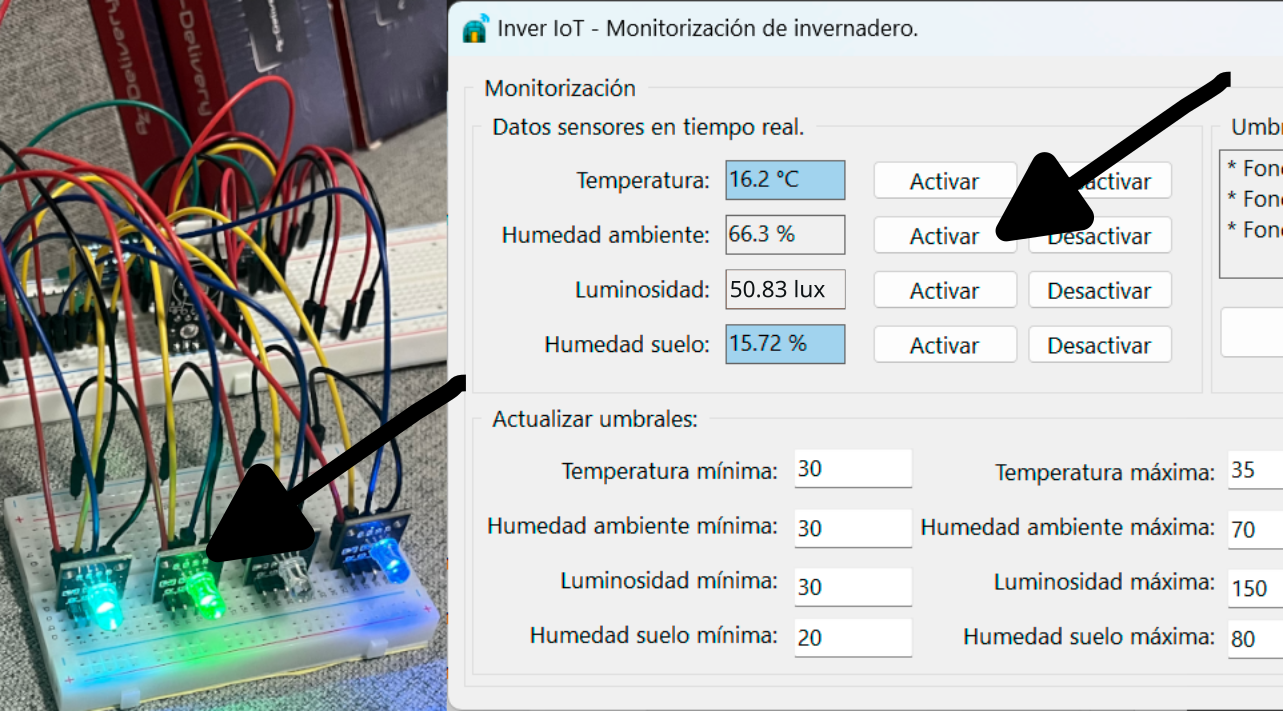
\includegraphics[width=0.61\textwidth]{img/desarrollo/InverIoT_verde_clickMecanismo.png}
	\caption{Al hacer clic en activar se enciende el led de color verde representando que estamos activando un mecanismo.}
\end{figure}

Sin embargo, la activación de mecanismos físicos como encender focos, activar calefacción, regar el suelo o humidificar el ambiente aún no se ha implementado, ya que corresponde a otras especialidades como telecomunicación industrial o mecánica.

El cannabis medicinal requiere condiciones ambientales constantes y dentro de un umbral específico para un crecimiento óptimo y delicado.

Definimos umbrales (valor mínimo/máximo) para mantener los valores de los sensores dentro de límites aceptables. En caso de detectar un valor anómalo fuera de estos umbrales, se genera una alerta. Para esta función, empleamos un bot de Telegram que envía mensajes de alerta, y se configura un LED RGB para cada medición (temperatura, humedad, luminosidad, humedad del suelo). Si la temperatura es baja, por ejemplo, el LED se ilumina en azul y envía una alerta por Telegram; si la temperatura es alta, el LED se enciende en rojo. Un LED apagado indica valores normales dentro del umbral.

\begin{table}[htbp]
\begin{center}
\caption{Umbrales ideales para un invernadero de cannabis medicinal.}
\begin{tabular}{|l|l|l|}
\hline
\rowcolor[HTML]{C0C0C0} 
\textbf{Característica} & \textbf{Mínimo} & \textbf{Máximo} \\ \hline
TEMPERATURA & 30 & 35\\ \hline
HUMEDAD & 30 & 70\\ \hline
LUMINOSIDAD & 30 & 150\\ \hline
HUMEDAD DEL SUELO & 20 & 80\\ \hline
\end{tabular}
\end{center}
\end{table}

La intervención manual también es posible, como activar ventiladores al observar un LED azul. Además, estos procesos pueden automatizarse. Por ejemplo, si la luminosidad cae por debajo del umbral, los focos se encienden hasta alcanzar el valor óptimo, por ahora eso no está implementado en este proyecto.

La información también se puede visualizar en tiempo real en una página web desarrollada con Node.js, incluyendo un histórico de datos almacenados en la base de datos.

A esta parte del proyecto se ha llamado \textbf{Dashboard} ~\ref{proyecto:Dashboard}.

La base de datos de la que extrae data el dashboard web es recopilada por lo que en este proyecto llamamos \textbf{NodeMqtt}~\ref{proyecto:NodeMqtt}.

%\begin{figure}[h]
	%\centering
	%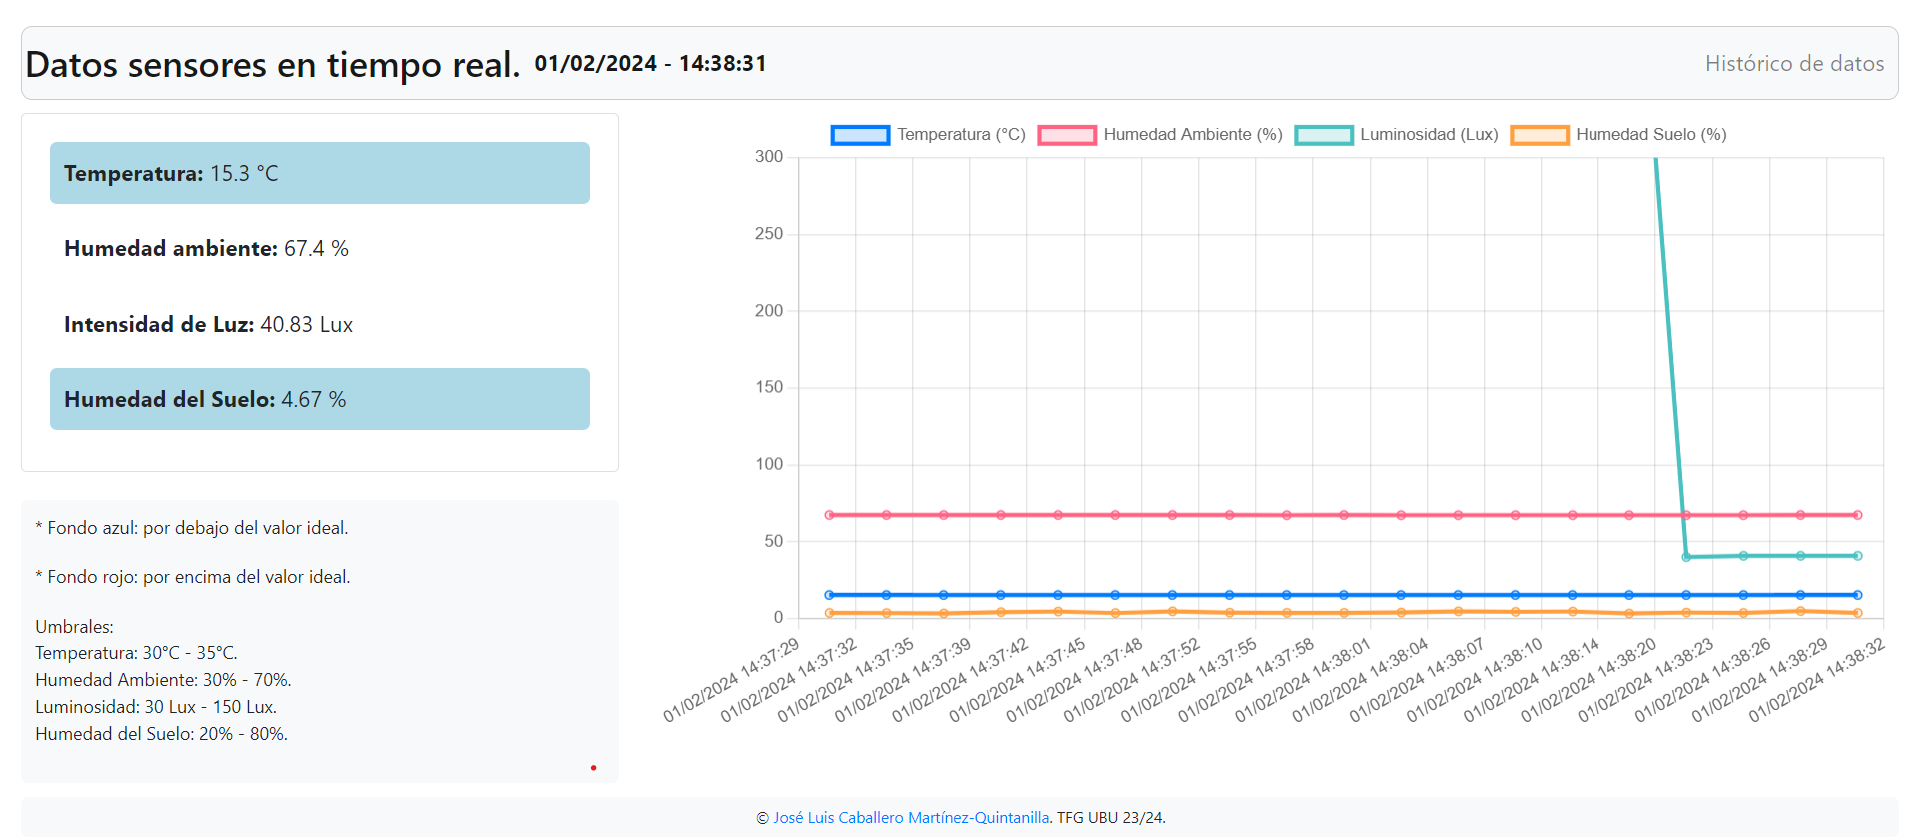
\includegraphics[width=1\textwidth]{img/desarrollo/Dashboard2.png}
	%\caption{Página Web \href{http://www.inveriot.com}{InverIoT} desarrollada con Node.js.}
%\end{figure}

%\begin{figure}[h]
	%\centering
	%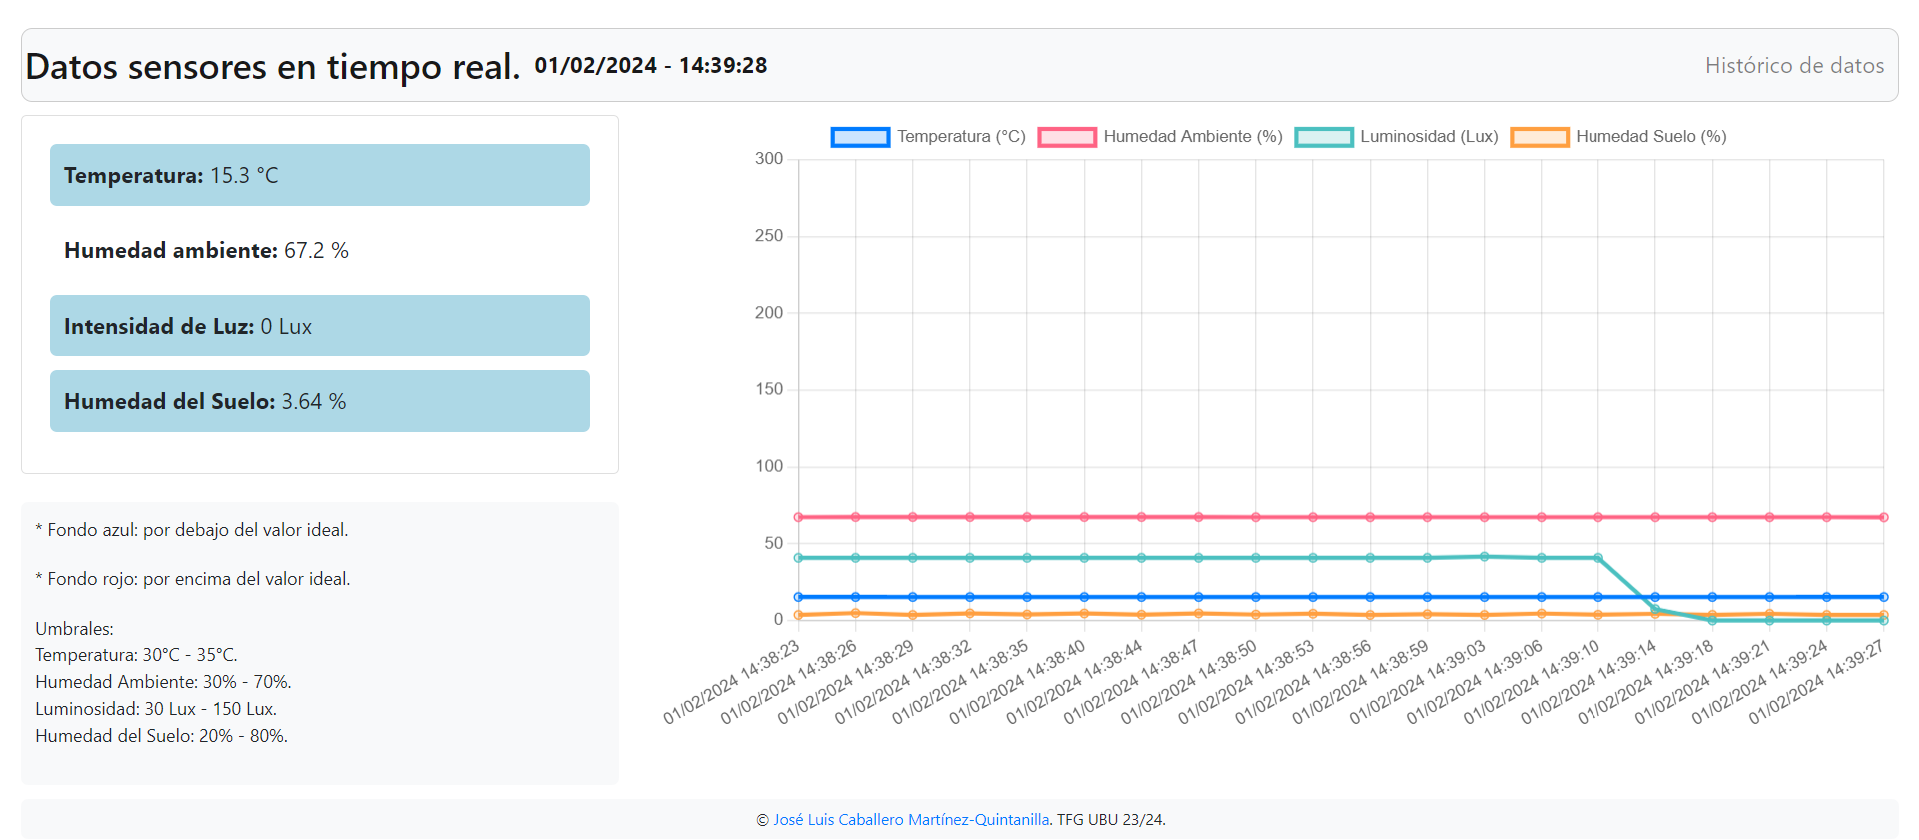
\includegraphics[width=1\textwidth]{img/desarrollo/Dashboard3.png}
	%\caption{Página Web \href{http://www.inveriot.com}{InverIoT} desarrollada con Node.js.}
%\end{figure}
%En este contexto, detallaré la configuración del servidor y la implementación de Node.js en la página web.

\subsection{Hardware}\label{proyecto:Hardware}
\begin{itemize}
	\item La Raspberry Pi Pico W estará situada en el invernadero para la recopilación de datos.
	\item Los LEDs RGB, instalados en la oficina del cliente, indicarán visualmente si los valores superan los umbrales establecidos.
	\item La pantalla OLED estará colocada en la puerta del invernadero para mostrar los valores actualizados.
\end{itemize}

\begin{figure}[h]
    \centering
    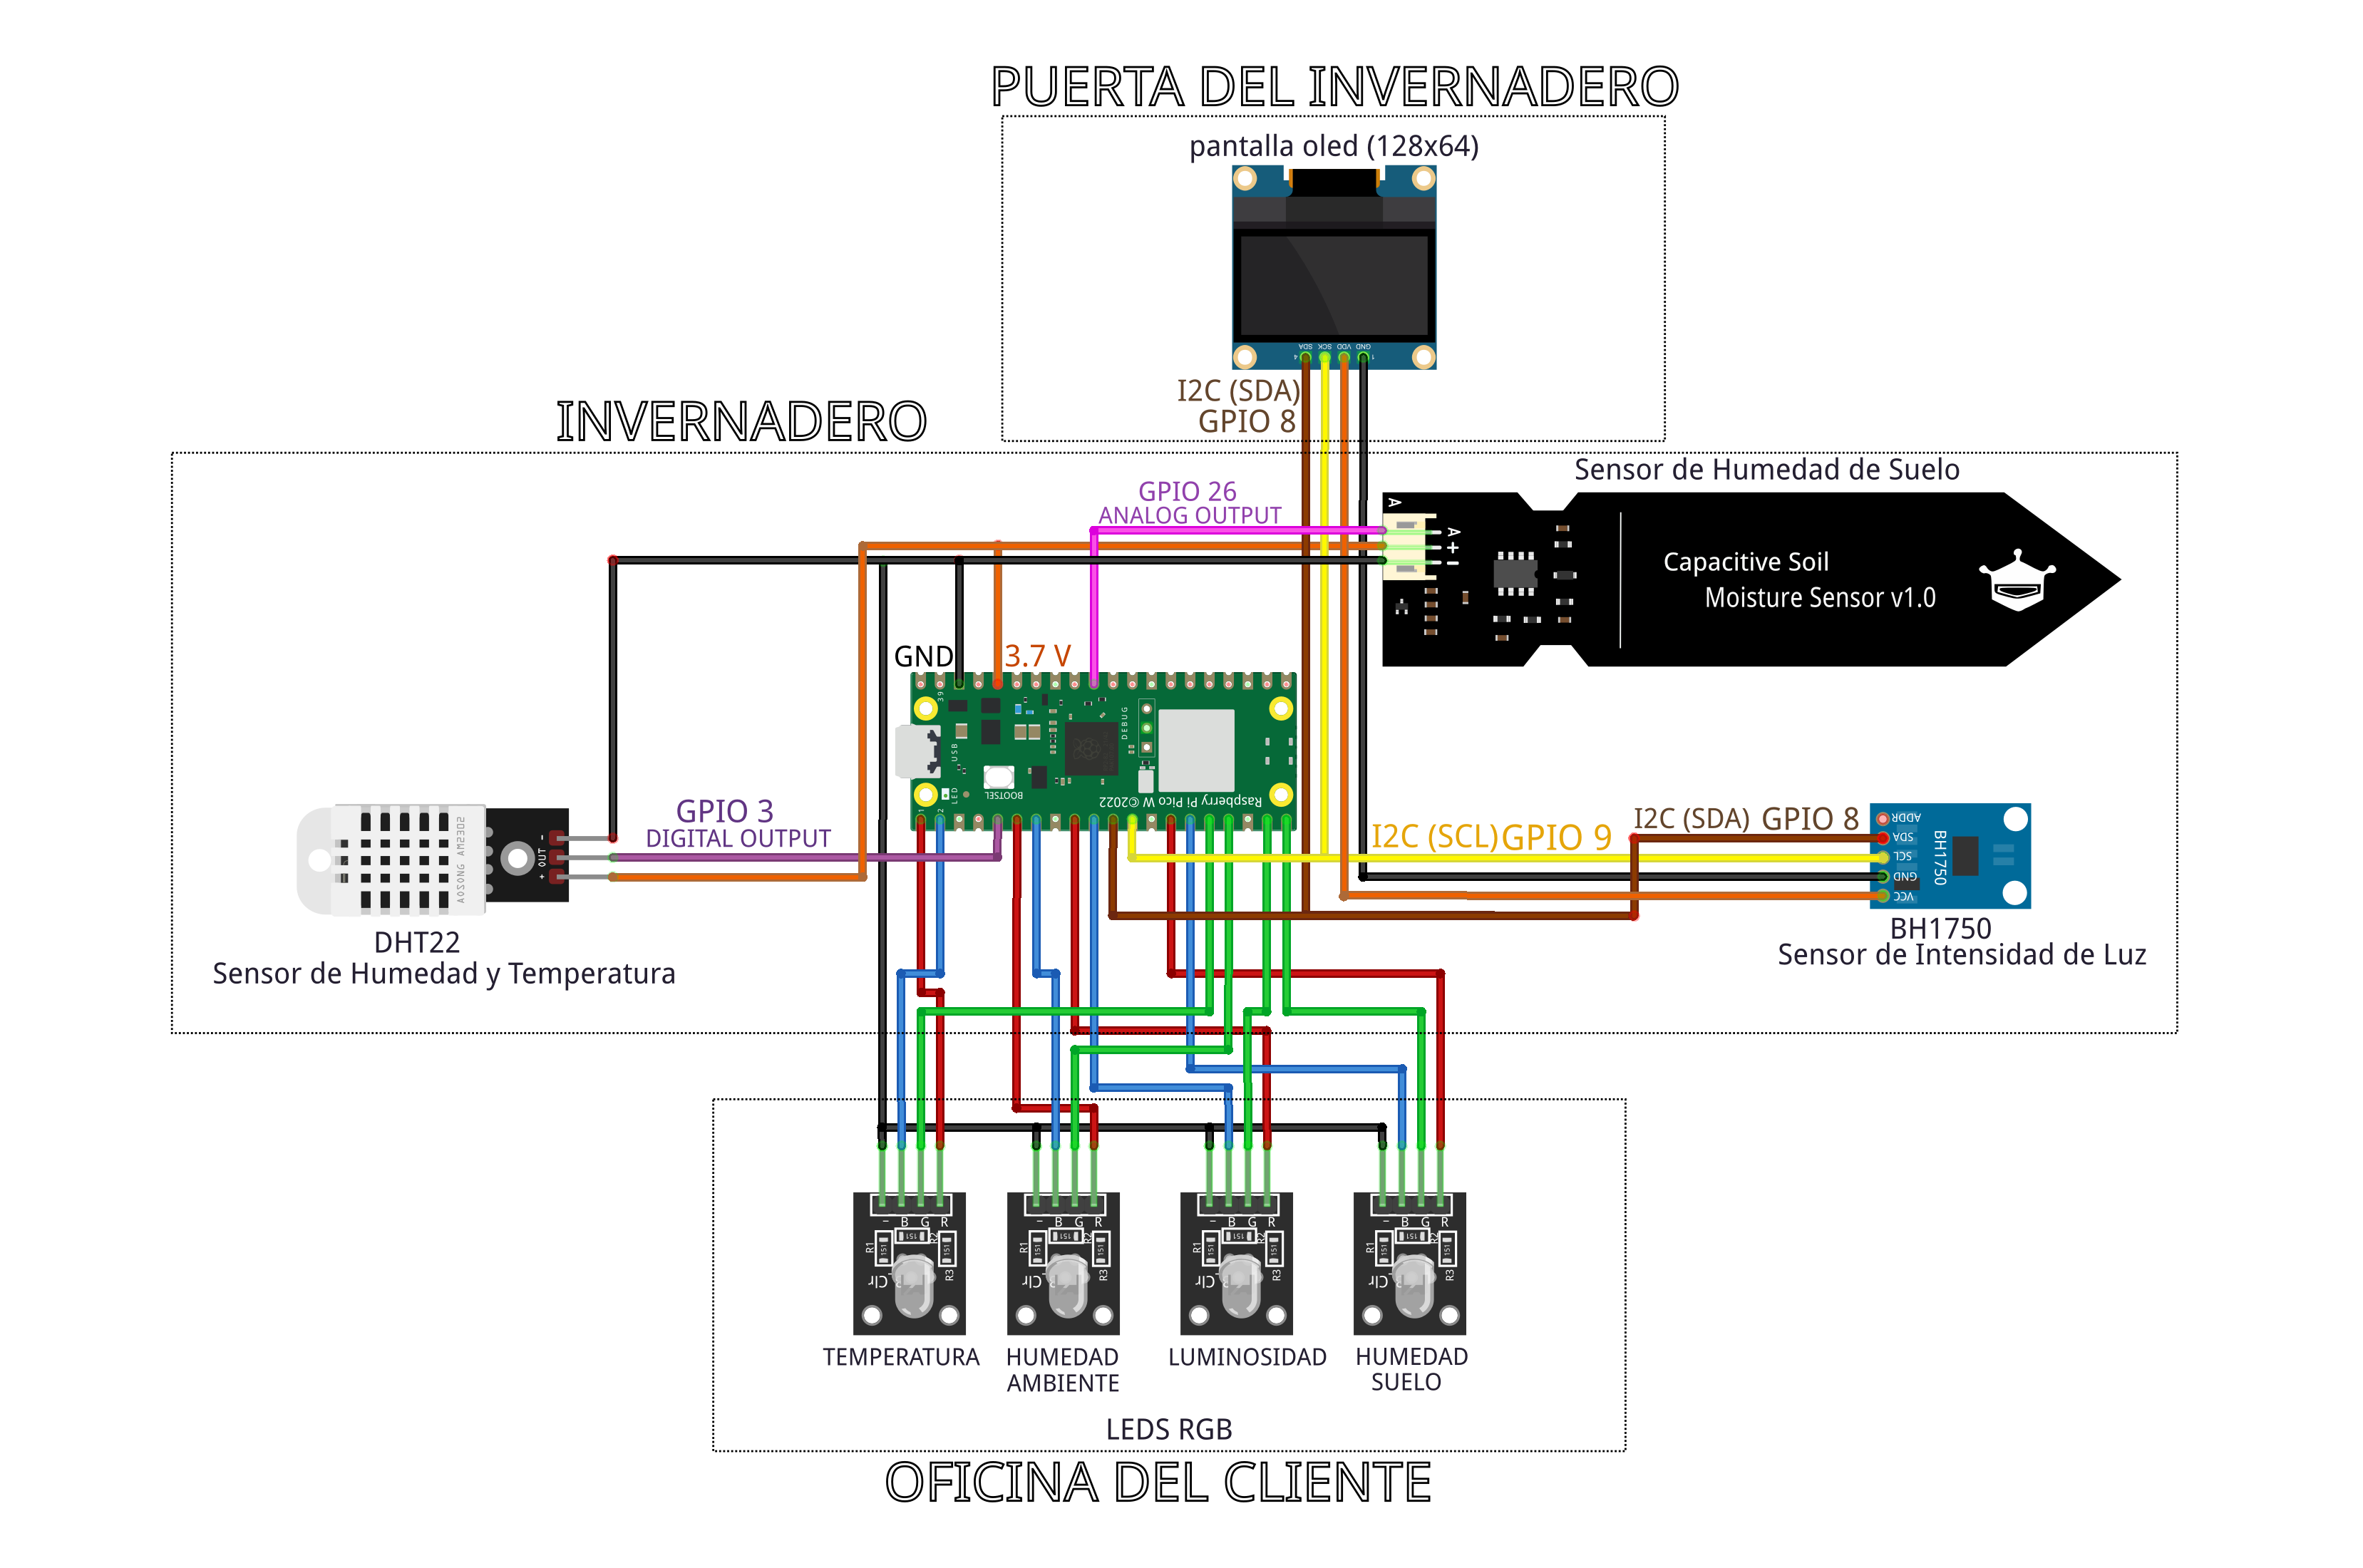
\includegraphics[width=1\textwidth]{img/diagramas/conexiones.png}
    \caption{Conexiones.} \label{Img:conexionesHardware}
\end{figure}
\pagebreak

\subsection{InverIoT}\label{proyecto:InverIoT}
Se desarrolla una aplicación de escritorio para Windows llamada InverIoT, que permite al usuario monitorizar en tiempo real los datos provenientes de los sensores conectados a la placa. 

\begin{figure}[h]
    \centering
    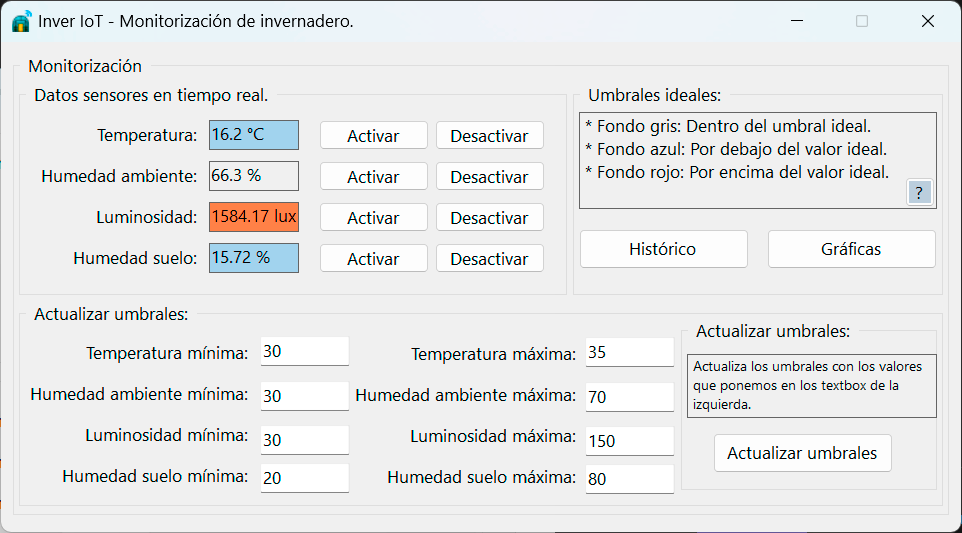
\includegraphics[width=0.95\textwidth]{img/desarrollo/InverIoT_Desktop.png}
	\caption{Aplicación de escritorio \textbf{InverIoT}.}
\end{figure}

Utilizando el protocolo MQTT~\cite{manual:MQTT}, la aplicación suscribe y recibe los datos publicados en el mismo tema. 

\begin{figure}[h]
    \centering
    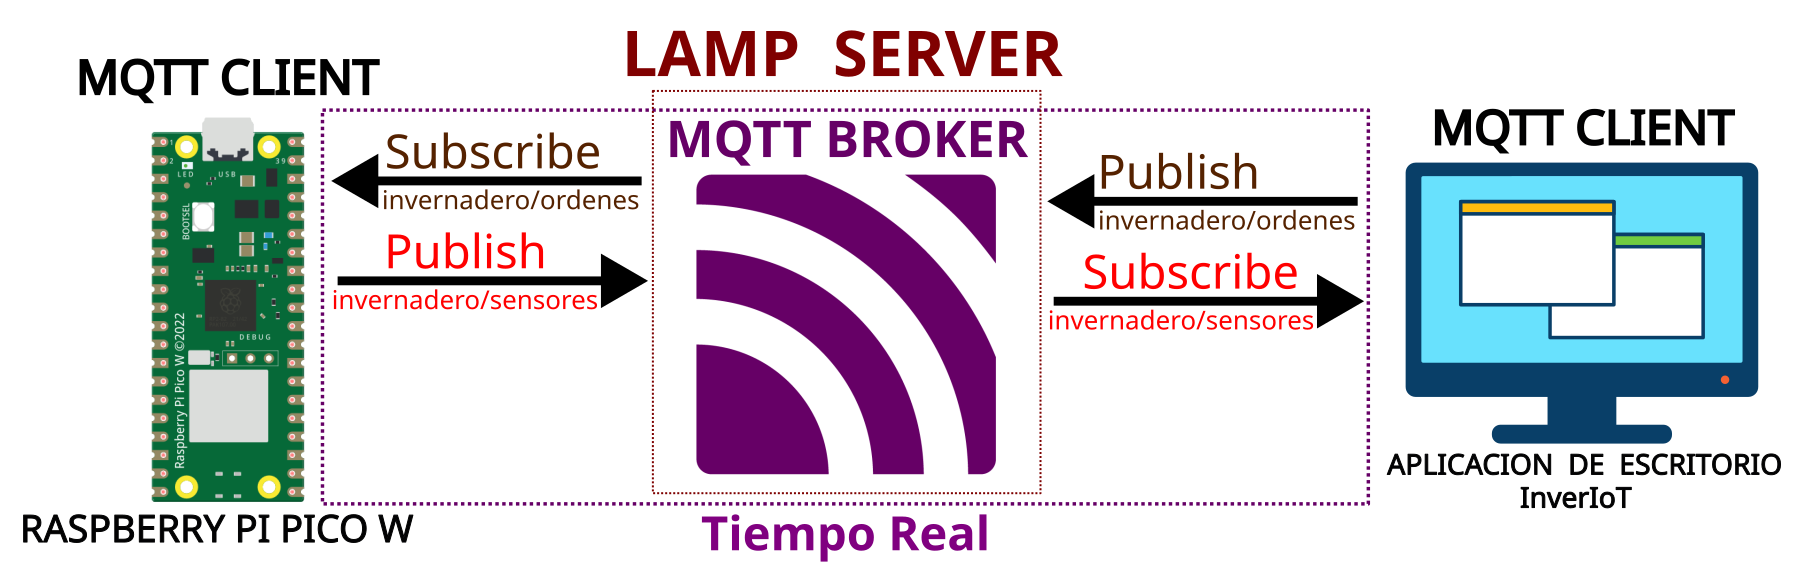
\includegraphics[width=0.95\textwidth]{img/diagramas/mqtt_InverIoT_TiempoReal.png}
    \caption{Enviando órdenes mediante MQTT la aplicación recibe datos en tiempo real.}
\end{figure}

\begin{figure}[h]
    \centering
    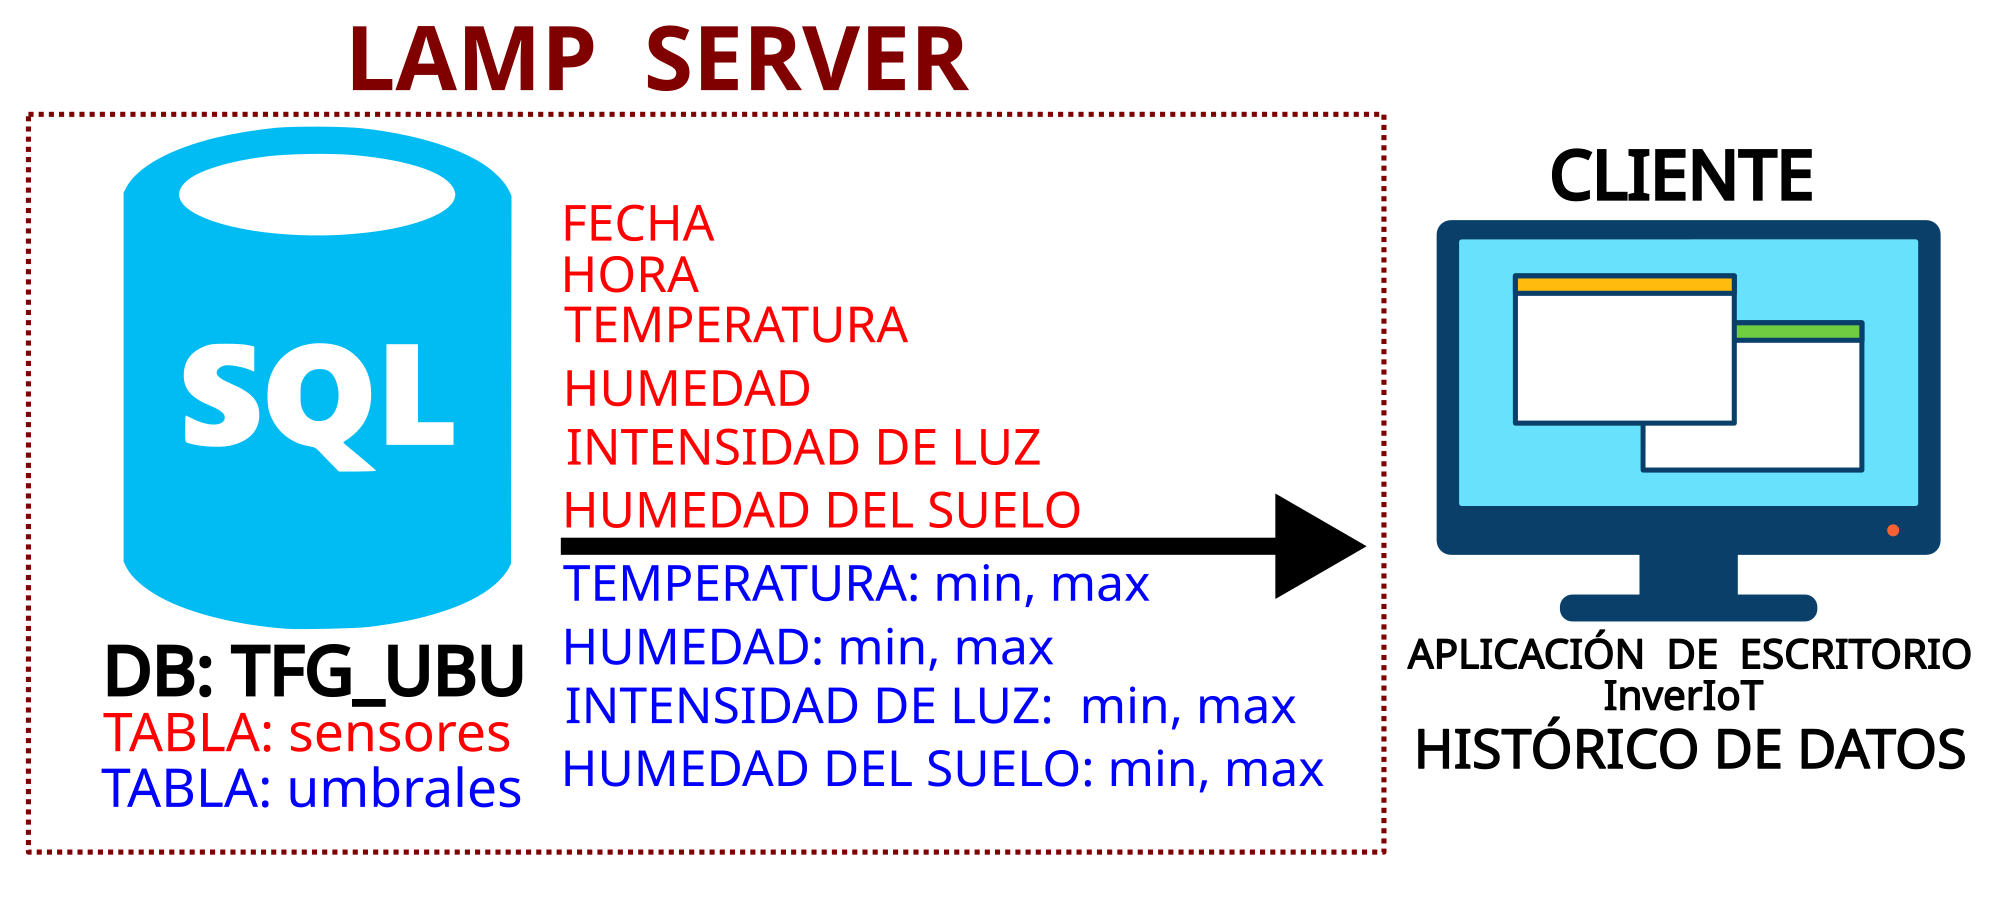
\includegraphics[width=1\textwidth]{img/diagramas/mqtt_InverIoT_Historico.png}
    \caption{Para mostrar el historial de datos la aplicación extrae información de una base de datos almacenada en un servidor LAMP.}
\end{figure}


Estos datos son formateados y presentados en textboxes correspondientes, con unidades de medida agregadas.

Se incorporan botones para activar o desactivar mecanismos, como un LED verde, que corrigen valores fuera de los umbrales ideales indicados en la parte derecha de la interfaz.

\begin{figure}[h]
    \centering
    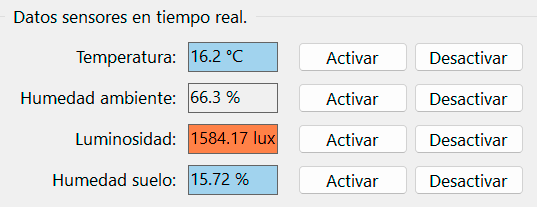
\includegraphics[width=1\textwidth]{img/desarrollo/InverIoT_Desktop_botones_control.png}
    \caption{Botones para activar o desactivar mecanismos.}
\end{figure}

Además, se añaden 8 textboxes en la parte inferior para ajustar manualmente los valores mínimos y máximos de cada parámetro.

Los umbrales se actualizan desde la base de datos del servidor LAMP, proporcionando indicadores visuales de color azul para valores bajos, gris para valores normales y rojo para valores altos.

Se desarrolló la aplicación de escritorio utilizando Windows Forms y programada en lenguaje \textbf{C\#}~\cite{manual:CSharp}.


La base de datos es alimentada por lo que en ese proyecto llamamos \textbf{NodeMqtt}~\ref{proyecto:NodeMqtt}, y la aplicación de escritorio \textbf{InverIoT} extrae esa información para mostrarla como un historial de datos.

La base de datos contiene dos tablas llamadas \textbf{sensores} y \textbf{umbrales}.

\begin{figure}[h]
    \centering
    \includegraphics[width=0.95\textwidth]{img/desarrollo/InverIoT_Histórico.png}
    \caption{Historial de los datos mostrara en la aplicación.}
\end{figure}


\begin{figure}[h]
    \centering
    \includegraphics[width=0.95\textwidth]{img/desarrollo/InverIoT_Gráficas.png}
    \caption{Gráfica mostrando los datos en un intervalo de fechas.}
\end{figure}
\pagebreak

\subsection{Dashboard}\label{proyecto:Dashboard}
Se desarrolla un dashboard que permite al usuario visualizar en tiempo real los datos capturados por los sensores, con una interfaz similar a la aplicación de escritorio.

Los valores que exceden los umbrales establecidos se destacan mediante cambios de color.

\begin{figure}[h]
    \centering
    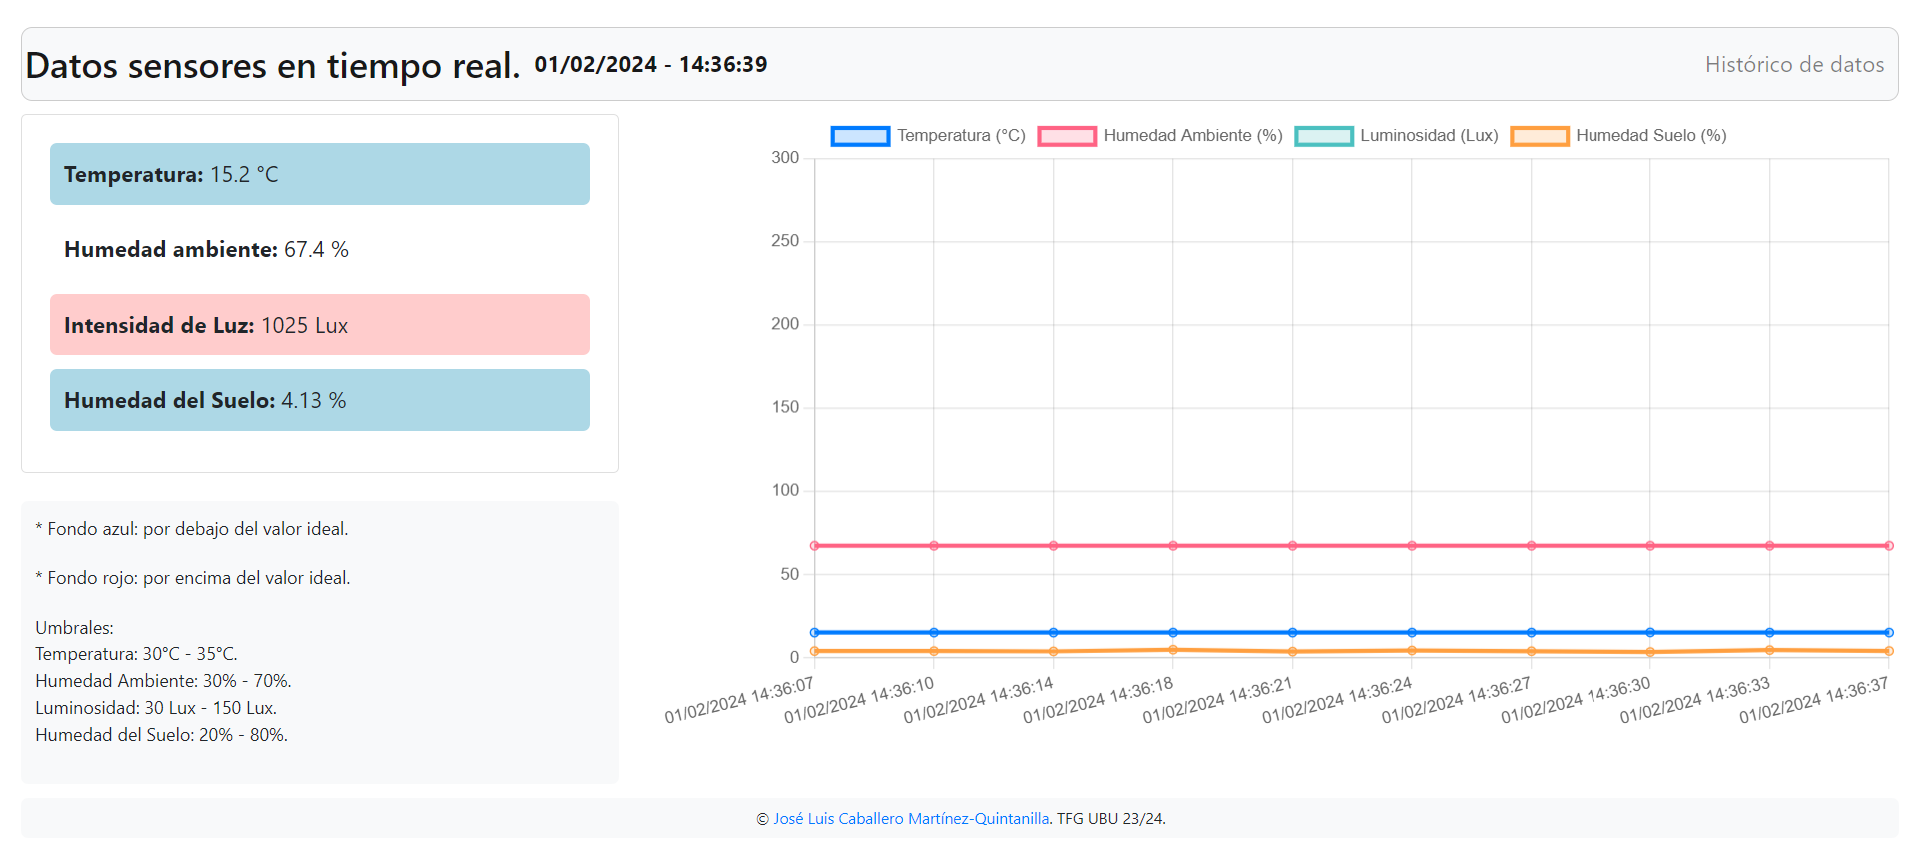
\includegraphics[width=0.95\textwidth]{img/desarrollo/Dashboard1.png}
    \caption{Intensidad de luz superando los umbrales.} \label{Img:Dashboard1}
\end{figure}

La plataforma incluye una gráfica en tiempo real y la capacidad de acceder a un historial con filtro de fecha.

\begin{figure}[h]
    \centering
    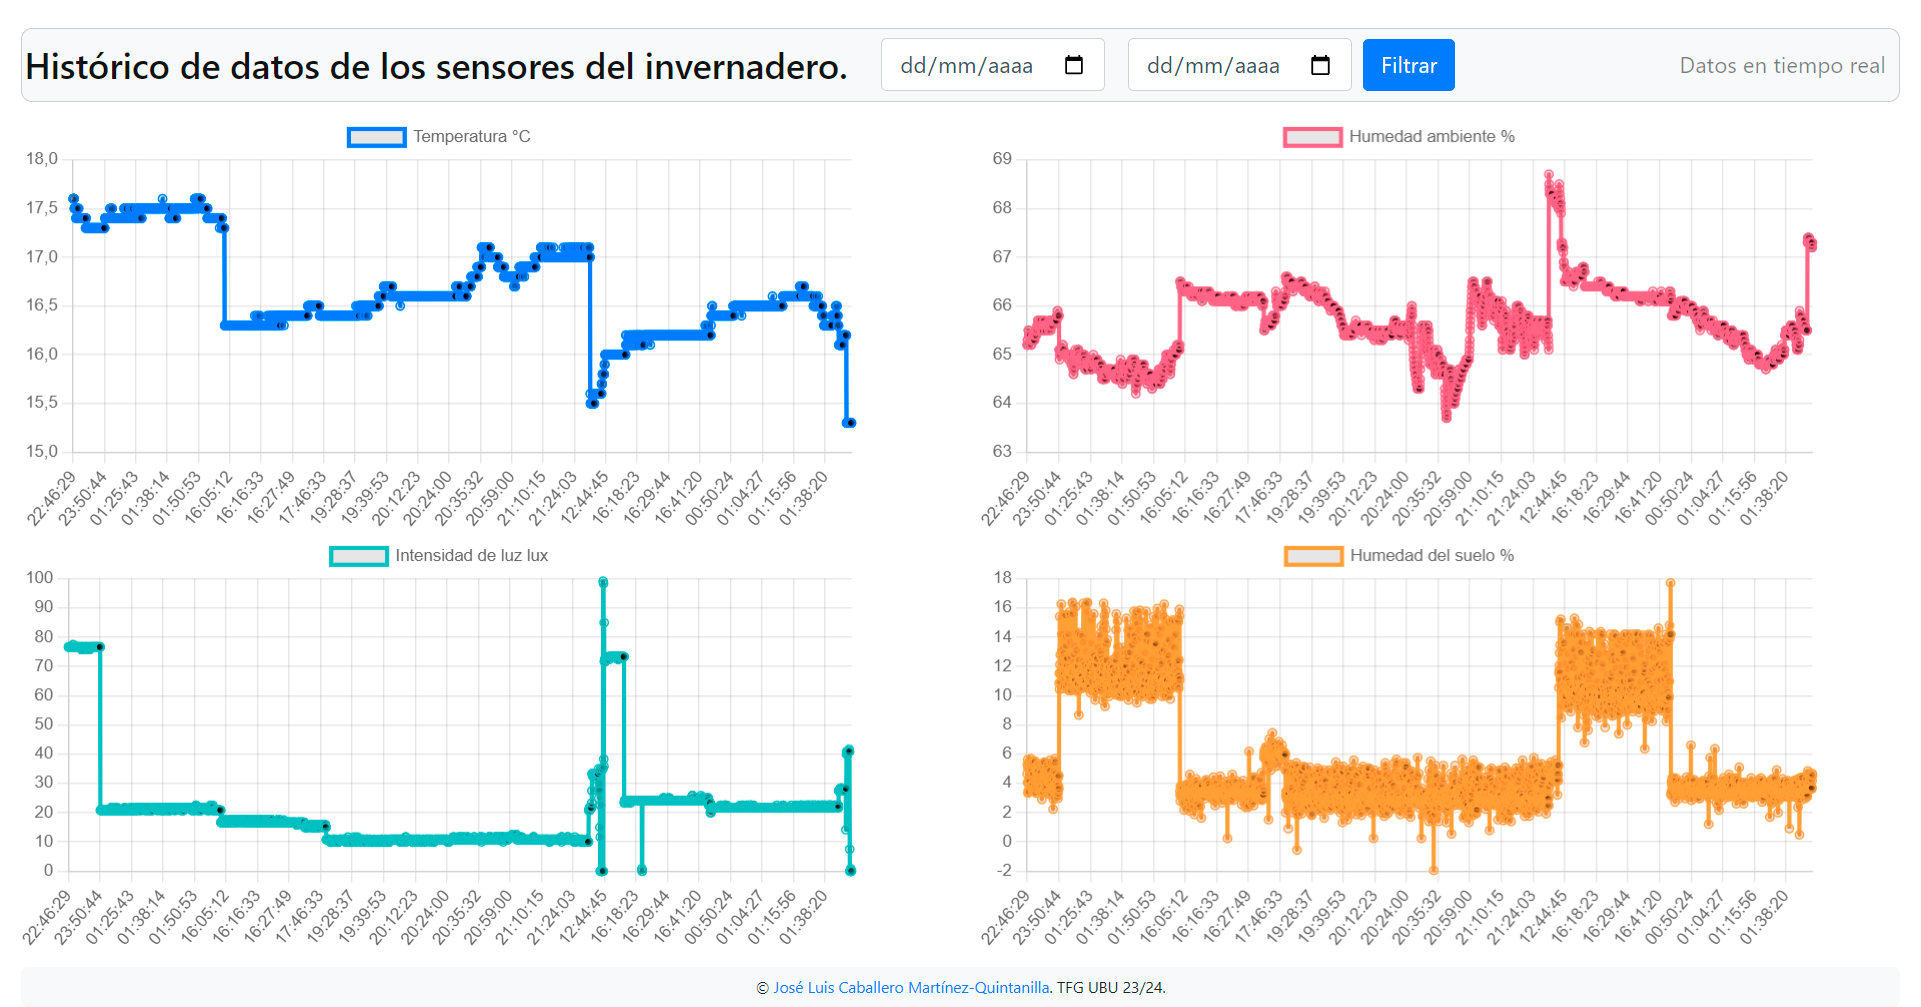
\includegraphics[width=0.95\textwidth]{img/desarrollo/Dashboard_Historico.png}
    \caption{Vista del historial, al cargar, muestra los datos del día actual.} \label{Img:Dashboard_Historico}
\end{figure}

Los umbrales utilizados se extraen de la tabla \textbf{TFG\_UBU} en la base de datos MySQL~\cite{misc:Mysql}.

\begin{figure}[h]
    \centering
    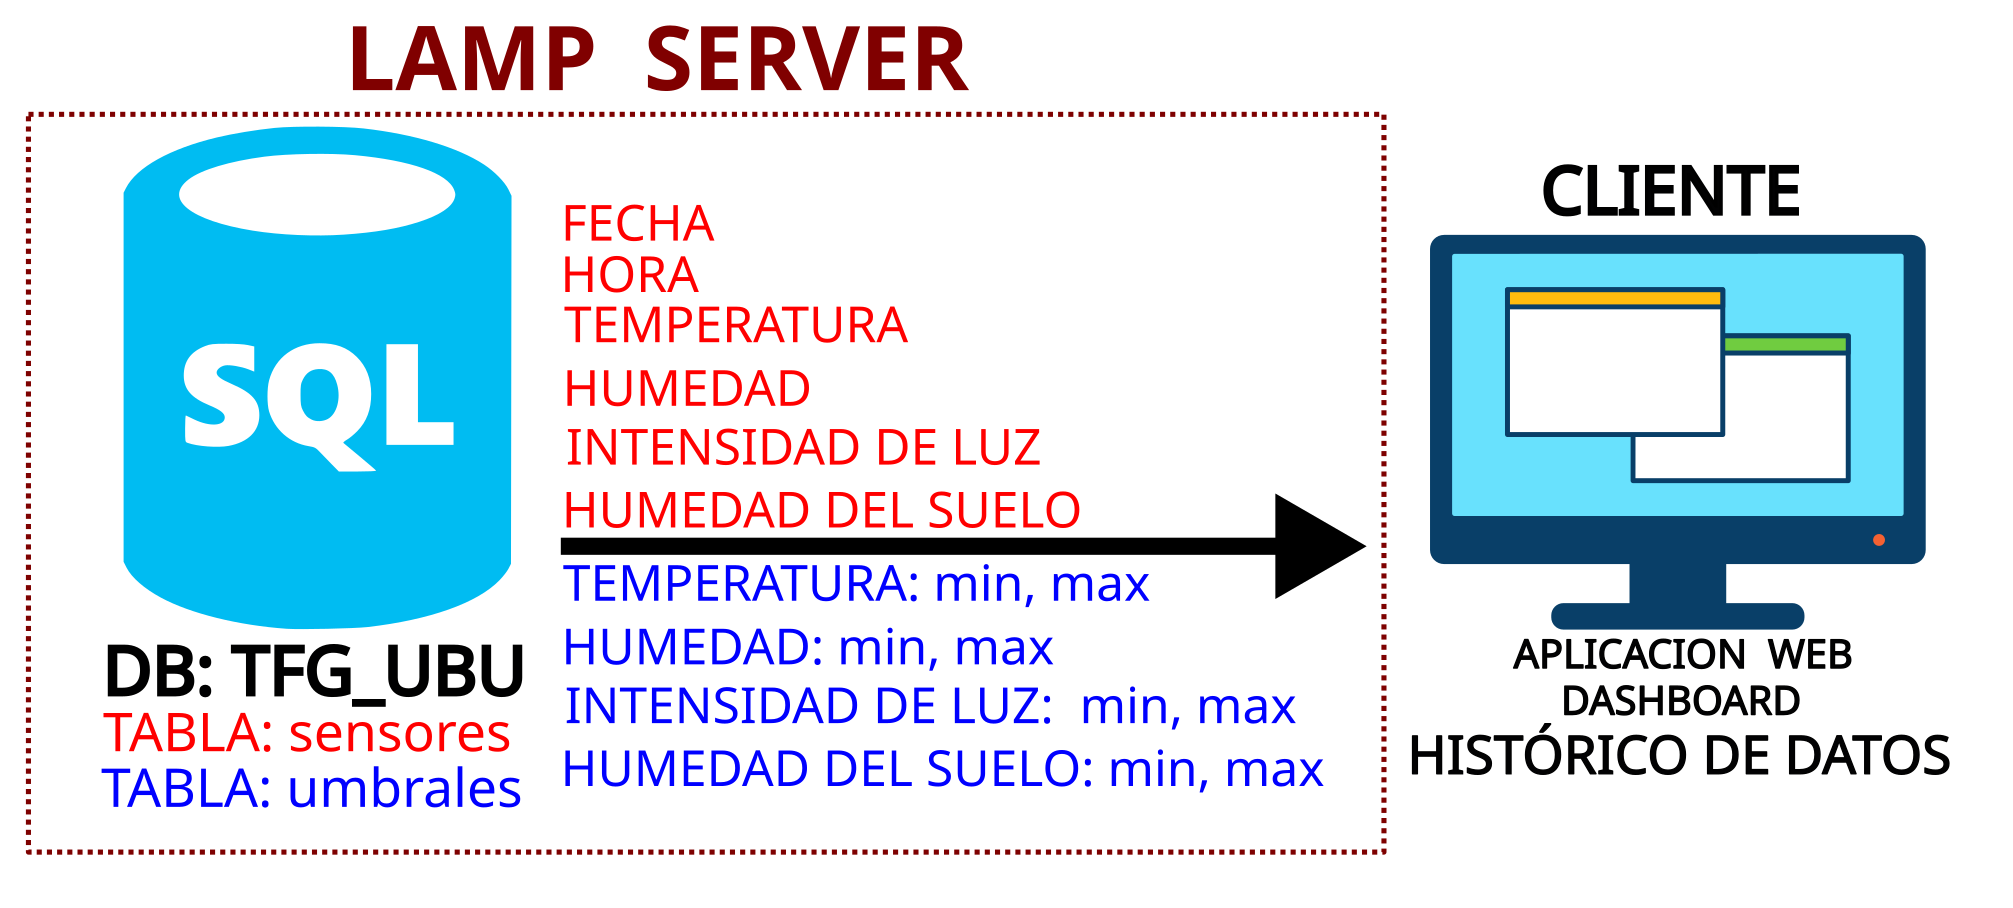
\includegraphics[width=1\textwidth]{img/diagramas/mqtt_dashboard_Historico.png}
    \caption{Extrae los datos de la base de datos para mostrar el historial.} \label{Img:Dashboard_diagrama_Historico}
\end{figure}

La Raspberry Pi Pico W utiliza una librería llamada \textbf{umqtt} para poder trabajar con MQTT, así es como envía data de los sensores y de los umbrales establecidos.

Los umbrales establecidos son almacenados en una base de datos que se encuentra en el servidor LAMP.

\begin{figure}[h]
    \centering
    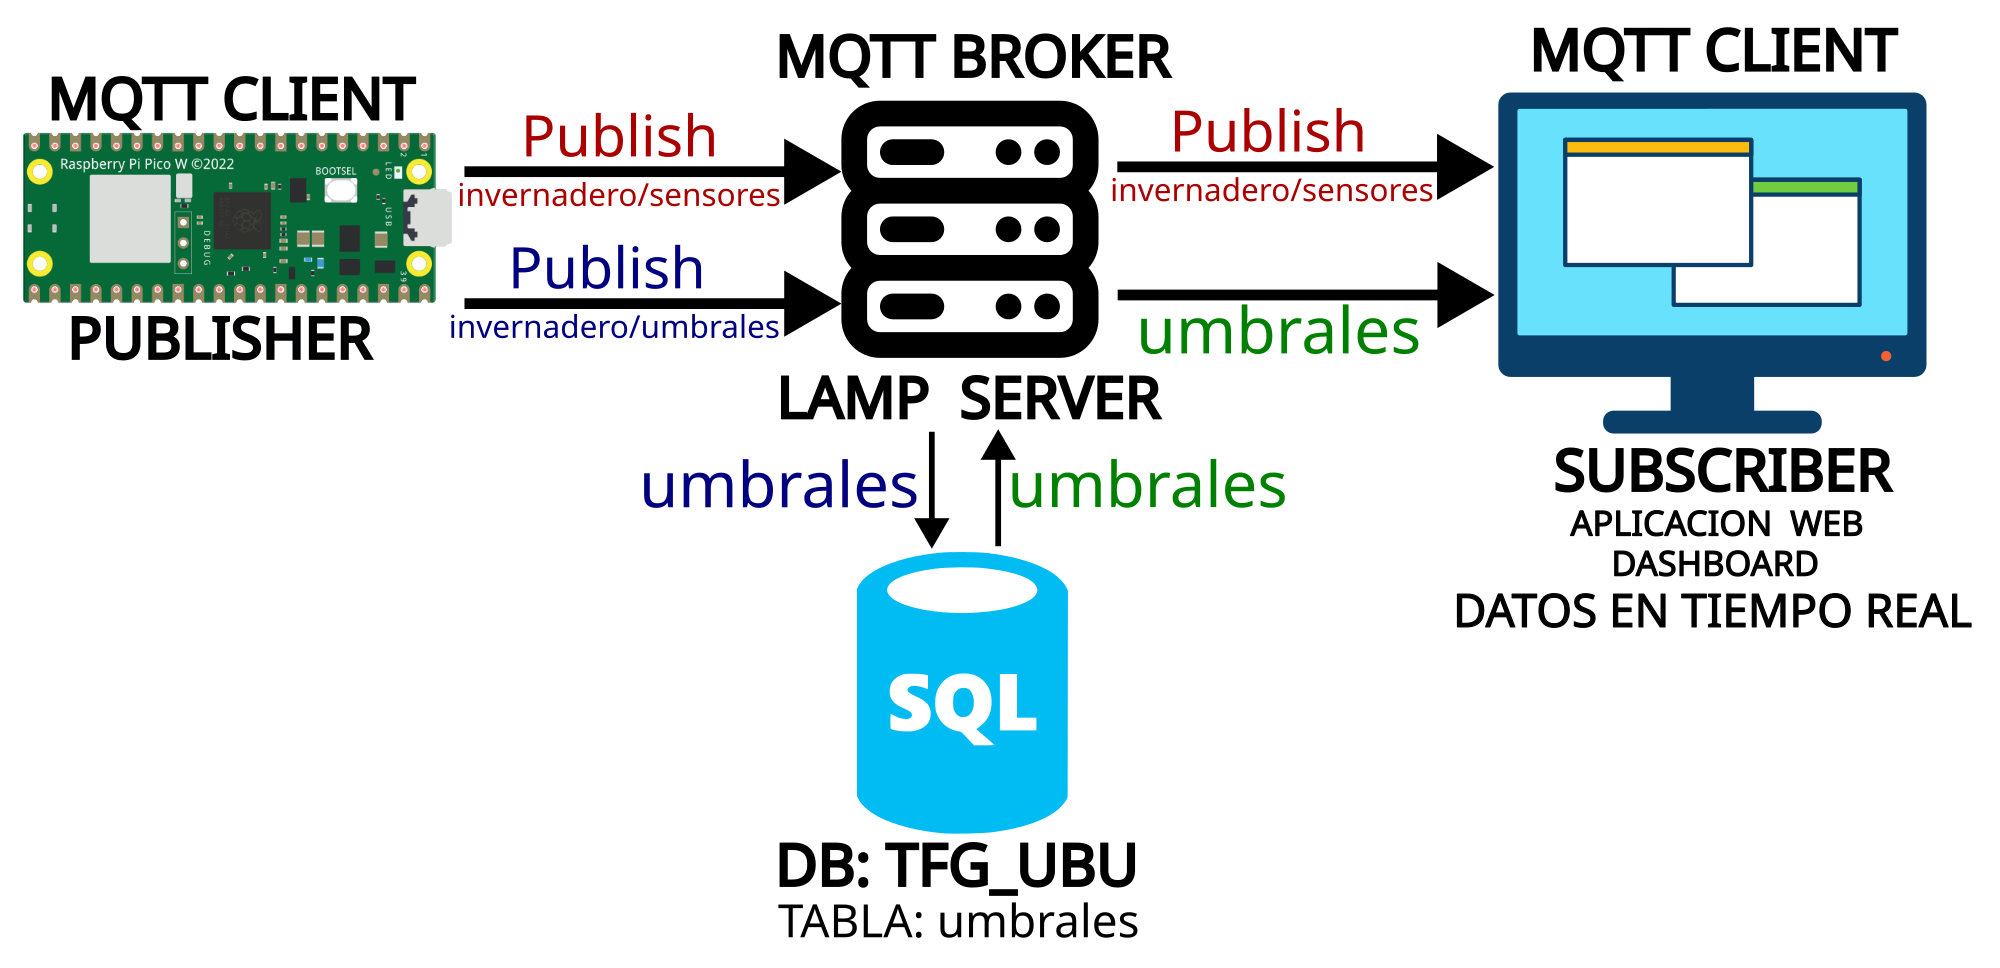
\includegraphics[width=1\textwidth]{img/diagramas/mqtt_dashboard_TiempoReal.png}
    \caption{Mediante MQTT extrae los datos para mostrarlos en tiempo real.} \label{Img:Dashboard_diagrama_TiempoReal}
\end{figure}

El panel de control está disponible para su acceso a través del siguiente enlace: \href{http://www.inveriot.com}{InverIoT Dashboard}



\subsection{NodeMqtt}\label{proyecto:NodeMqtt}
\textbf{nodeMqtt} es un servicio en Node.js~\cite{misc:Nodejs} que escucha los topics \textbf{invernadero/sensores} e \textbf{invernadero/umbrales}. Utiliza la librería MQTT.js~\cite{misc:MQTTjs}. Los datos son enviados por la placa Raspberry Pi Pico W RP2040~\cite{misc:RPiPicoW}, que recopila valores de sensores. El servicio \textbf{nodeMqtt} captura, formatea y luego inserta estos datos en la base de datos MySQL~\cite{misc:Mysql} para los valores de sensores, además de actualizar los umbrales correspondientes.

Está conformado por los siguientes archivos:

\begin{itemize}
	\item \textbf{index.js:}
		Es el punto de entrada del código de la aplicación.
	\item \textbf{package.json:}
		Es un archivo de configuración que describe la aplicación y sus dependencias.
\end{itemize}

\begin{figure}[h]
	\centering
	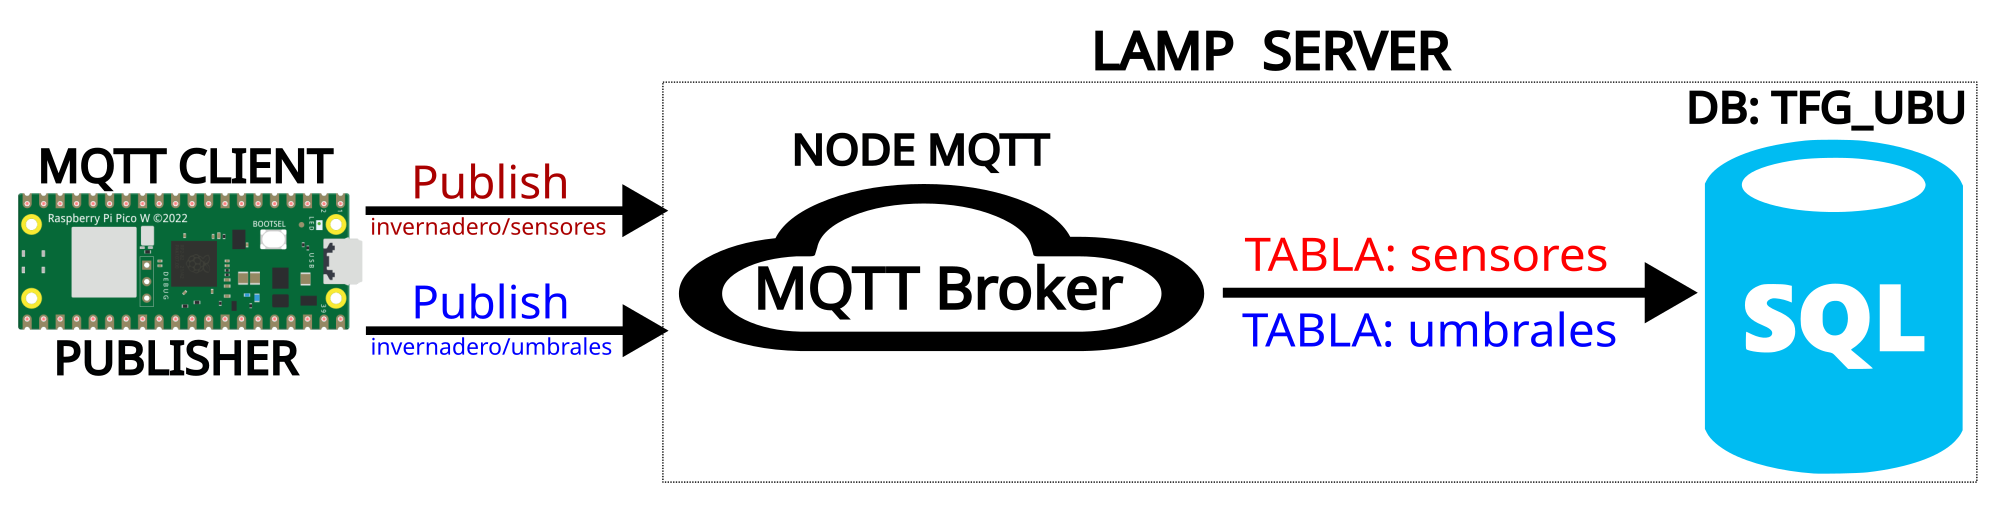
\includegraphics[width=1\textwidth]{img/diagramas/mqtt_nodeMqtt.png}
	\caption{MQTT con Node.js para almacenar datos de los sensores.}
\end{figure}

%Este apartado pretende recoger los aspectos más interesantes del desarrollo del proyecto, comentados por los autores del mismo.
%Debe incluir desde la exposición del ciclo de vida utilizado, hasta los detalles de mayor relevancia de las fases de análisis, diseño e implementación.
%Se busca que no sea una mera operación de copiar y pegar diagramas y extractos del código fuente, sino que realmente se justifiquen los caminos de solución que se han tomado, especialmente aquellos que no sean triviales.
%Puede ser el lugar más adecuado para documentar los aspectos más interesantes del diseño y de la implementación, con un mayor hincapié en aspectos tales como el tipo de arquitectura elegido, los índices de las tablas de la base de datos, normalización y desnormalización, distribución en ficheros3, reglas de negocio dentro de las bases de datos (EDVHV GH GDWRV DFWLYDV), aspectos de desarrollo relacionados con el WWW...
%Este apartado, debe convertirse en el resumen de la experiencia práctica del proyecto, y por sí mismo justifica que la memoria se convierta en un documento útil, fuente de referencia para los autores, los tutores y futuros alumnos.

%\capitulo{6}{Trabajos relacionados}

Para comprender plenamente la contribución y novedad de este proyecto, es esencial explorar investigaciones y desarrollos previos relacionados.

\subsection{Monitorización de la energía consumida mediante Raspberry Pi para sistema domótico}\label{Proy1}

Se trata de un TFG desarrollado en la Universidad Carlos III de Madrid que trata sobre un sistema de monitorización de energía consumida para una instalación domótica mediante el uso de una Raspberry Pi, en el que se debe realizar el diseño del circuito y la programación correspondientes para poder extraer datos de diez sensores de corriente de forma simultánea.

Cada sensor recoge información correspondiente a una línea del cuadro de electricidad donde irá instalado.

En el desarrollo de este proyecto se pueden diferenciar dos partes:

\begin{itemize}
\item Montaje del circuito que lleva los datos obtenidos de los sensores de corriente hacia la Raspberry Pi para que puedan ser gestionados adecuadamente.

\item Configuración de la Raspberry Pi para la lectura y procesado de los datos obtenidos a través de cada uno de los sensores. Tales datos son guardados en diferentes ficheros dependiendo del canal de los que provengan, denominados datos\_canalX.txt, donde X es el número del sensor.
\end{itemize}

Introduciendo un comando determinado el sistema es capaz de:

\begin{itemize}
	\item Modificar el tiempo existente entre el recojo de cada muestra para un canal específico, que es guardado en un fichero de tiempos para su continua lectura.
	\item Recoger datos a partir de un canal, fecha y hora, de forma que se lee el fichero datos\_canalX correspondiente al canal introducido, y se guardan en otro fichero todos aquellos datos posteriores a la fecha y hora introducidos.
\end{itemize}

Podemos ver su referencia en la bibliografía en la referencia~\cite{TesisBaron2017}.

En la columna \textbf{Proy1} de la tabla~\ref{tabla:comparativa-proyectos} podemos ver algunas características de este proyecto.

\subsection{Diseño e implementación de un sistema domótico basado en Raspberry Pi}\label{Proy2}

Se trata de un TFG desarrollado en la Universidad Carlos III de Madrid que trata sobre un sistema domótico de bajo coste, basado en código libre (UNIX/LINUX). Dicho sistema permite al usuario manejar de forma fácil y sencilla elementos finales como motores y leds.

El elemento de software principal es el sistema operativo Raspbian (basado en Debian), aunque ahora es llamado Raspberry Pi OS. Tal sistema operativo es instalado en la RaspberryPi.

El segundo elemento software importante es el servidor web Apache que gestiona la aplicación web desarrollada bajo el patrón de desarrollo Modelo-Vista-Controlador (MVC).

El sistema domótico está compuesto por varios sus-sistemas:

\begin{itemize}
	\item La aplicación web.
	\item La base de datos.
	\item El conjunto de sensores y actuadores.
\end{itemize}

La aplicación web se ha desarrollado sobre un servidor LAMP que es accesible desde el exterior y que actua de interfaz sobre el usuario del sistema domótico y le propio sistema.

Algunas acciones que puede realizar el usuario mediante este sistema:

\begin{itemize}
	\item Consultar temperatura y humedad.
	\item Controlar apertura puertas/persianas.
	\item Consultar histórico de temperaturas y humedades.
	\item Consultar movimiento en una habitación.
	\item Controlar iluminación interior.
\end{itemize}

Podemos ver su referencia en la bibliografía en la referencia~\cite{TesisSantos2017}.

En la columna \textbf{Proy2} de la tabla~\ref{tabla:comparativa-proyectos} podemos ver algunas características de este proyecto.

\section{Fortalezas y debilidades este proyecto}

Las fortalezas clave del proyecto son:

\begin{itemize}
	\item Todos los elementos utilizados en este proyecto son fácilmente accesibles, tanto en términos de software como de hardware.
	\item La elección de la Raspberry Pi Pico W fue crucial gracias a su bajo consumo de energía, su compacto tamaño que facilita la portabilidad y su capacidad de conectividad Wifi.
	\item La versatilidad de la Raspberry Pi Pico W, con su capacidad de conectividad Wifi, ha posibilitado tanto el envío de datos como la recepción de órdenes. Además, su flexibilidad se evidencia en la implementación exitosa de MQTT en el proyecto.
	\item La modularidad del sistema permite una fácil escalabilidad, ya que es posible agregar nuevos sensores o funcionalidades sin mayores complicaciones.		
	\item La presentación gráfica de datos en tiempo real en una pantalla OLED y la posibilidad de acceder a través de una aplicación de escritorio y un panel web ofrecen múltiples formas de acceder y visualizar la información recopilada.
\end{itemize}

Las principales debilidades de este proyecto son:

\begin{itemize}
	\item La prueba del sistema se realizó en un ambiente no controlado, lo que puede afectar la precisión de los datos y la generación de alertas. Esto podría limitar la fiabilidad de las respuestas del sistema en condiciones reales.
	\item La funcionalidad del proyecto está intrínsecamente ligada a la conectividad Wifi de la Raspberry Pi Pico W. Problemas en la red Wifi podrían afectar la transmisión de datos y la recepción de órdenes.
	\item Aunque se han incluido sensores relevantes, la variedad podría ser limitada. La adición de más tipos de sensores podría mejorar la capacidad de monitoreo y la precisión de los datos recopilados.
	\item A medida que se agregan más sensores y funcionalidades, la capacidad de la Raspberry Pi Pico W podría alcanzar sus límites. En proyectos a mayor escala, se podría requerir hardware más potente.
\end{itemize}

\begin{table}[htbp]
\centering
\begin{tabular}{lccc}
\toprule
Características & MICM & Proy1 & Proy2  \\
\midrule
Proyecto libre & \cellcolor{green!25} {\checkmark} & \cellcolor{green!25} {\checkmark} & \cellcolor{green!25} {\checkmark} \\
Menor precio en modelo de Raspberry Pi & \cellcolor{green!25} {\checkmark} & \cellcolor{red!25} {\xmark} & \cellcolor{red!25} {\xmark} \\
Menor consumo de energía de Raspberry Pi & \cellcolor{green!25} {\checkmark} & \cellcolor{red!25} {\xmark} & \cellcolor{red!25} {\xmark} \\
Escalabilidad & \cellcolor{green!25} {\checkmark} & \cellcolor{green!25} {\checkmark} & \cellcolor{green!25} {\checkmark} \\
Modularidad & \cellcolor{green!25} {\checkmark} & \cellcolor{green!25} {\checkmark} & \cellcolor{green!25} {\checkmark} \\
Más opciones de visualización de datos & \cellcolor{green!25} {\checkmark} & \cellcolor{red!25} {\xmark} & \cellcolor{red!25} {\xmark} \\
Mayor potencia en modelo de Raspberry Pi & \cellcolor{red!25} {\xmark} & \cellcolor{green!25} {\checkmark} & \cellcolor{green!25} {\checkmark} \\
Más opciones de acceso de datos & \cellcolor{green!25} {\checkmark} & \cellcolor{red!25} {\xmark} & \cellcolor{red!25} {\xmark} \\
Interacción multiplataforma             & \cellcolor{green!25} {\checkmark} & \cellcolor{green!25} {\checkmark} & \cellcolor{green!25} {\checkmark} \\
WiFi entre elementos                    & \cellcolor{green!25} {\checkmark} & \cellcolor{green!25} {\checkmark} & \cellcolor{green!25} {\checkmark \\
Almacenamiento de datos                    & \cellcolor{green!25} {\checkmark} & \cellcolor{green!25} {\checkmark} & \cellcolor{green!25} {\checkmark} \\
\bottomrule
\end{tabular}
\caption{Comparativa de las características de los proyectos.}
\label{tabla:comparativa-proyectos}
\end{table}

%Este apartado sería parecido a un estado del arte de una tesis o tesina. En un trabajo final grado no parece obligada su presencia, aunque se puede dejar a juicio del tutor el incluir un pequeño resumen comentado de los trabajos y proyectos ya realizados en el campo del proyecto en curso. 

%\capitulo{7}{Conclusiones y Líneas de trabajo futuras}

Todo proyecto debe incluir las conclusiones que se derivan de su desarrollo. Éstas pueden ser de diferente índole, dependiendo de la tipología del proyecto, pero normalmente van a estar presentes un conjunto de conclusiones relacionadas con los resultados del proyecto y un conjunto de conclusiones técnicas. 
Además, resulta muy útil realizar un informe crítico indicando cómo se puede mejorar el proyecto, o cómo se puede continuar trabajando en la línea del proyecto realizado. 


\bibliographystyle{plain}
\bibliography{bibliografia}

\end{document}
